\documentclass[]{report}
\usepackage[top=1in, bottom=1in, left=1.25in, right=1.25in, includehead]{geometry}
\pagestyle{headings}
\usepackage{setspace}
\usepackage[utf8]{inputenc} % this is needed for umlauts
\usepackage[T1]{fontenc}    % this is needed for correct output of umlauts in pdf

\usepackage{array}
\usepackage{longtable}
\usepackage{amsmath, amsthm, amstext, amssymb, amsfonts}
\usepackage{rotating}
\usepackage[hidelinks]{hyperref}
\usepackage{color}
\usepackage{float}
\usepackage{multirow}
\usepackage{wasysym}
\usepackage{graphicx}
\usepackage{listings}
\usepackage[noend]{algpseudocode}
\usepackage{empheq}
\usepackage{multicol}
\usepackage{xparse}
\usepackage{url}
\usepackage{pdfpages}
\usepackage{subcaption}
\makeatletter
\setlength{\@fptop}{0pt}
\newcommand{\code}[1]{\texttt{#1}}
\usepackage[dvipsnames]{xcolor}
\usepackage{textcomp}
\usepackage{fontspec}
\usepackage[normalem]{ulem}
\useunder{\uline}{\ul}{}
\usepackage{longtable}
\usepackage{colortbl}
\usepackage{hhline}
\usepackage{todonotes}
\usepackage{url}
\urlstyle{same}
\usepackage{algorithm}
\let\svalgorithm\algorithm
\catcode`'=\active
\catcode`"=\active
\def\quoteactive{\catcode`'=\active\def'{\makebox{\textquotesingle}}}
\def\qquoteactive{\catcode`"=\active\def"{\makebox{\textquotedbl}}}
\catcode`'=12
\catcode`"=12
\def\algorithm{\quoteactive\qquoteactive\svalgorithm}
\makeatother

\renewcommand{\arraystretch}{1.3}

%%%%%%%%%%%%%%%%%%%%%%%%%%%
%% Thesis body           %%
%%%%%%%%%%%%%%%%%%%%%%%%%%%

\begin{document}

%%%%%%%%%%%%%%%%%%%%%%%%%%%
%% Title page            %%
%%%%%%%%%%%%%%%%%%%%%%%%%%%
\begin{titlepage}
$\;$
\vskip1.5in
\onehalfspacing

\begin{center}
{\LARGE
Typeface Space: Neural Networks for Font Selection
}
\large
\vskip.175in
by\\
Samuel Magid\\
\vskip.125in
Professor Jeannie Albrecht, Advisor\\
Professor Mark Hopkins, Advisor\\
\singlespacing
\vskip.5in
\small
A thesis submitted in partial fulfillment\\
of the requirements for the\\
Degree of Bachelor of Arts with Honors\\
in Computer Science\\
\vskip.5in
Williams College\\
Williamstown, Massachusetts\\
\vskip.5in
\today
%%\vskip.5in
%%{\Huge \textbf{DRAFT}}
\end{center}
\end{titlepage}

%%%%%%%%%%%%%%%%%%%%%%%%%%%%%%

\setcounter{page}{2}
\tableofcontents
\clearpage
\phantomsection
\addcontentsline{toc}{chapter}{List of Figures}
\listoffigures
\clearpage
\phantomsection
\addcontentsline{toc}{chapter}{List of Tables}
\listoftables
\onehalfspacing

%%%%%%%% Chapters %%%%%%%%%%%%
\clearpage
\chapter*{Abstract}
\label{chap:abstract}

Over the past forty years, surprisingly little progress has been made on user font selection. Whereas the number of fonts available to users has increased by several orders of magnitude, the font selection interface of almost every major word processor and design tool has remained the same: an scrollable, alphabetized list of font names. This interface does not provide users with any ability to search for fonts based on style---a problem since users often look for fonts matching certain style characteristics---and is an increasingly unfeasible method of search as the number of available fonts continues to increase. This project attempts to address this problem, hypothesizing that training autoencoder-like neural networks on font image data will yield meaningful quantitative style encodings for typefaces, upon which useful font selection interfaces can be built. We implement three models of increasing complexity---our Basic Autoencoder model, a Style Transfer model incorporating vector character embeddings as model input, and a model adapted from Srivatsan et al.\ \cite{srivatsan2020} which utilizes convolution and variational encoding---and find that the model adapted from Srivatsan et al.\ and trained on our full dataset is highly capable of representing a wide variety of typeface styles. We implement an end-to-end font selector webapp based on these model style encodings, and find preliminary results in a small user study suggesting that our user tool based on the model style encodings effectively allows users to locate and select fonts based on style characteristics.
\clearpage
\chapter*{Acknowledgements}
\addcontentsline{toc}{chapter}{Acknowledgements}
\label{chap:acknowledgements}

This thesis has been a significant undertaking, and I am deeply grateful to the people who have supported me in this process. To my friends and family, I appreciate your kindness as I have grown increasingly fixated on this niche topic. Thank you for listening as I talked through many of my ideas---the good ones and the bad ones. To the Williams Computer Science Department, thank you for the institutional support that made this thesis possible, as well as the wonderful community you have all provided. To my thesis advisors, Mark and Jeannie, thank you for being the best advisors I could ask for, encouraging my creativity, giving me support and guidance when I needed it, and helping me get to the finish line of this project. And to everyone else in my life who I have not yet mentioned, thank you for helping me at every stage to grow into the person I am today.
%% Introduction
\chapter{Introduction}
\label{chap:introduction}

\section{Motivation}

According to Karen Cheng's 2006 book \textit{Designing Type,} there were, at the time of publishing, likely over 300,000 individual typefaces available to users \cite{cheng2006}. Today, almost twenty years later, that number is no doubt higher; and yet, we use essentially the same font selection tools developed decades ago: a scrollable list of font names. All major word processors (Microsoft Word, Apple Pages, Google Docs) and most other graphic design tools use this decades-old interface. A few improvements have been made on the basic list-based font selection model (e.g. displaying font names in their own typeface and list alphabetization), but the fundamental aspects of the interface have remained unchanged. Here there arises an issue: compared with these early word processors, users have access to several orders of magnitude more typefaces---hundreds of thousands compared to dozens. Users cannot be expected to navigate through such a large number of fonts; scrolling through 300,000 items is not a reasonable ask. Moreover, this list-based interface does not align with the typical needs of a user: when searching for fonts, users often have a particular style in mind (professional, casual, festive), and this basic list-based interface does not incorporate any notion of style as part of its search. Notably, alphabetical order in a list of typefaces does not help a user who does not already know the name of the font they are searching for. After over forty years of little development in the area of font selection interfaces---while the numbers of available fonts has increased substantially---there is a need for better font selection tools, particularly interfaces which take into account meaningful aspects of typeface style.

\section{Goals and Contributions}

This thesis aims to address this problem. We show that training autoencoder-like neural networks on font image data yields meaningful style encoding vectors which quantify different aspects of typeface style, upon which useful style-based font selection tools can be built. We implement three neural network models, all variants of an autoencoder, which encode typeface style in the intermediate vector representation between the autoencoder's encoding and decoding blocks. Using the style encodings from the most effective model, we build a novel font selection webapp that leverages spatial information from the model. Evaluating our models' encoding spaces using attribute categories provided by Google Fonts, we find that our models effectively encode certain aspects of style, with similarity scores within style categories increasing as model sophistication increases. We additionally conducted a font-matching user study comparing our font selection tool against two baselines; while we are not able to draw conclusions about quantitative performance between tools given the small size of our user study, the qualitative feedback we collected suggests that our font selector webapp provided several desireable aspects for font exploration.

Ultimately, we find that the models we have implemented, especially our final model adapted from Srivatsan et al. \cite{srivatsan2020} and trained on our full dataset, effectively encode many aspects of typeface style. We additionally demonstrate---based on the preliminary findings from our user study---that these style encodings can be used to create useful style-based font selection interfaces. This research contributes to the field of typeface style inference and suggests that further work can be done towards the issue of creating effective and simple style-based font selection tools.

\section{Roadmap}

This thesis document is organized as follows. Chapter 2 explores some of the background and history of font selection tools, looking at early font selection interfaces as well as a couple of recently developed language-based tools; explains the structure of autoencoders and autoencoder-like models; and reviews related work on font selection and font inference. Chapter 3 details our three models (Basic Autoencoder, Style Transfer, and our model adapted from Srivatsan et al.), explains how we obtain the style encodings used by our font selection tool, discusses the design choices for our novel font selector interface, and details the end-to-end system upon which the tool is built. Chapter 4 includes a quantitative evaluation of font distance similarity based on attribute categories from the Google Fonts library, as well as a user evaluation of our font selection tool. Chapter 5 summarizes our findings, enumerates a few areas for future work, and explains some of the lessons learned in the process of this extended research project.
%% Background
\chapter{Background}
\label{chap:background}

In this chapter, we provide necessary background to contextualize our research. Our Font Selection section explores the history of font selection tools, identifying a few recent areas of development which vary from the common list-based interface. In Autocoders, we introduce the autoencoder model and its variations, laying the fundamental structure for the neural network models we implement in this work. Finally, in Previous Work, we review related work on font selection and font inference, discussing important contributions which have informed our model design and system implementation.

\section{Font Selection}

This section explores some important background information about the history and current state of font selection tools. Comparing one of the earliest font selection interfaces---from the built-in word processor on the 1981 Xerox Star---to the typical font selection interfaces on Google Docs, Microsoft Word, and Apple Pages, it is evident that little progress has been made in the way we select fonts. Nevertheless, there has been some recent innovation in typeface selection interfaces, and we explore some of these new approaches---specifically the new language-based font selection models of the Google Fonts website and Canva, a popular online graphic design tool. We additionally discuss the difficulty of creating language-based font selection tools. Lastly, we provide an analogue between font selection interfaces and the much more diverse field of color selection, another common selection in graphic design, to envision alternative modeling schema for font selection.

\subsection{Lack of Development in Font Selection Interfaces}

Surprisingly little progress has been made in the past several decades on user font selection. Figure \ref{fig:xerox-star} shows the font selection interface on the 1981 Xerox Star, one of the earliest personal computers to include a multi-font word processor. This interface will probably look familiar to a modern user: it provides control over font size; bold, italic, underline, and strikethrough toggles; superscript and subscript options; and, importantly, a scrollable list of fonts to choose between. Compared to the modern font selection interfaces shown in Figure \ref{fig:font-selectors}, the only significant difference over this 44-year gap is the alphabetization of the font selector list; otherwise, these interfaces are practically identical. While there are many beneficial aspects of this interface---control over size, boldness, and other useful dimensions of typeface---the list-based typeface selector has become increasingly unfit for the task of font selection. Whereas the Xerox Star provided its users with a small number of typefaces to choose between, today the number of individual typefaces available to users (although impossible to enumerate exactly) almost certainly exceeds 300,000 \cite{cheng2006}. It is not feasible for a user to scroll through this many typefaces when making a font selection. Additionally, this interface provides little guidance about style: in an alphabetized list, there is no particular relationship between nearby fonts, or any capability for style-based search. This leads users to find a few fonts they like and stick with them, rather than explore the wide variety available to them. Without a better tool for navigating the many dimensions of typeface style, this will remain the case.

% from Designing the Xerox “Star” User Interface, Byte, issue 4, 1982
\begin{figure}
    \centering
    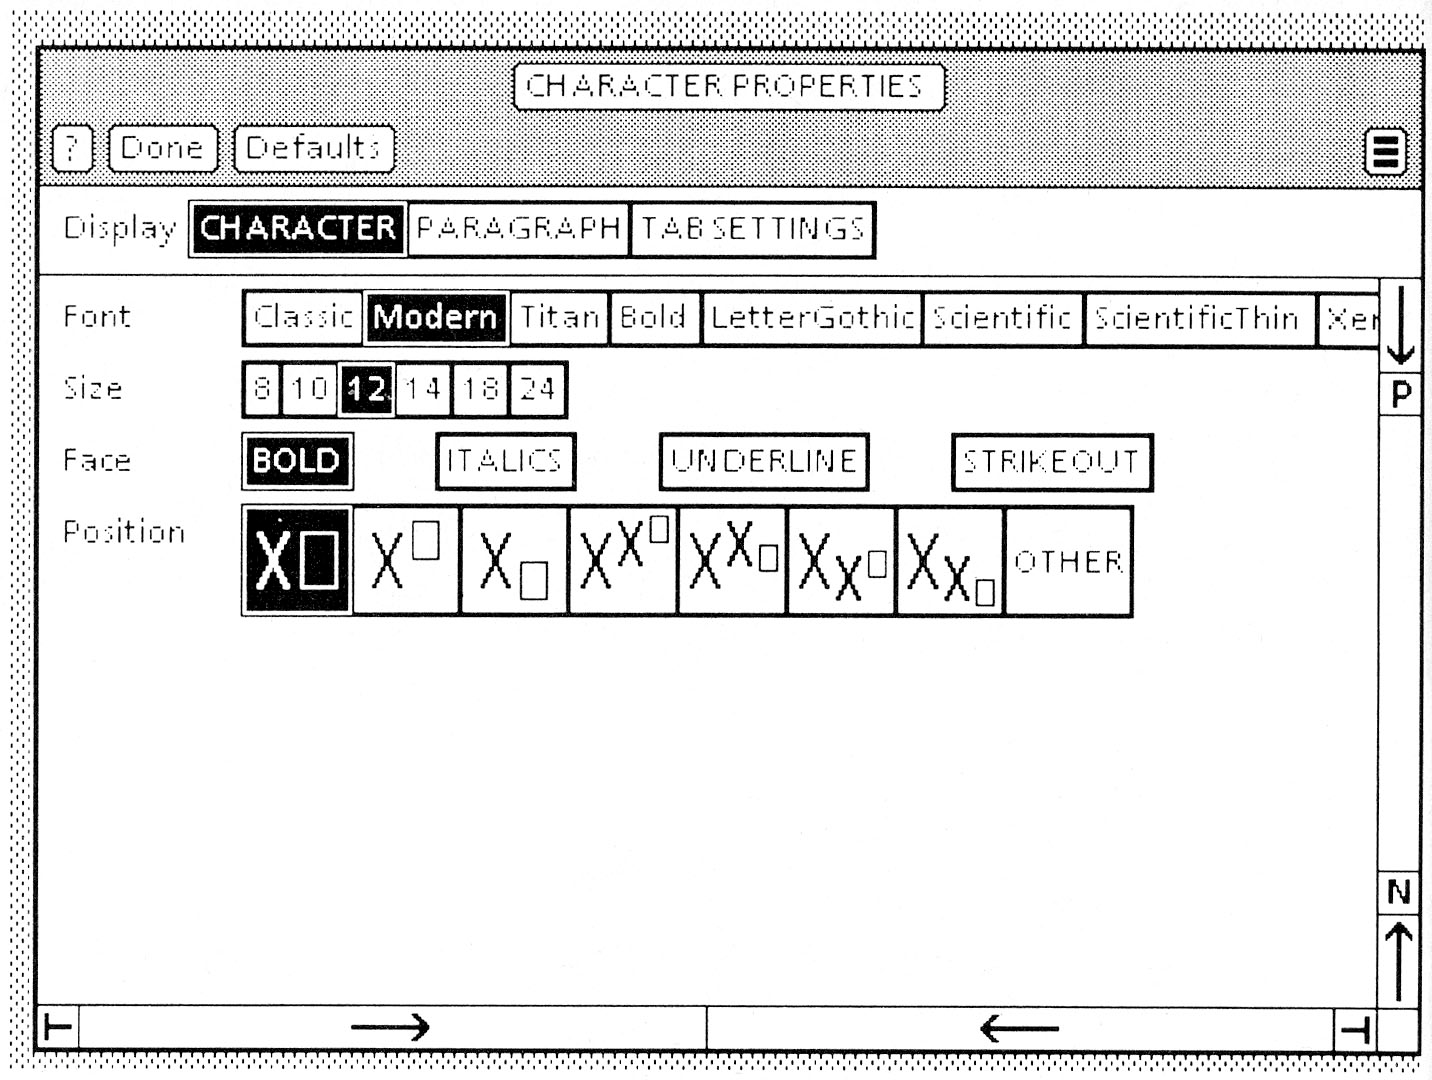
\includegraphics[width=.8\textwidth]{images/xerox-star.png}
    \caption{Font selection interface in Xerox Star (1981)}
    \label{fig:xerox-star}
\end{figure}

O'Donovan et al.\ \cite{odonovan2014} lists several reasons for the difficulty of developing font selection tools. The first issue, as discussed above, is the sheer number of available fonts. ``Most computers are now equipped with hundreds of fonts,'' they note, while online resources provide access to hundreds of thousands. Another issue is a lack of obvious ways to categorize fonts in a manner which corresponds to user goals. While there exist broad categories like Serif, Sans Serif, and Handwritten, these must be manually designated on a per-font basis, and they are not necessarily helpful to every user. A college student, for example, might know to choose a Serif font for their paper to convey an academic mood—or, more practically, to fulfill certain departmental design expectations—however another user, looking to design a new logo for their coffee shop, might not find the distinction between Serif, Sans Serif, and Handwritten typeface particularly useful or informative. Typical users lack the tools, given the current state of font selector interfaces, to properly consider the wide range of typefaces and confidently choose the right font—one of the most fundamental decisions in effective text-based graphic design. Finally, users vary in their font selection goals. One user may be looking to identify the font they saw on a store sign or a brochure—or to find a free-to-use font which is similar to a commercial one they have identified---while another may be looking to match a particular mood, or to choose a font that fits well with the rest of their document. A third may simply be exploring a large set of fonts like Adobe TypeKit or Google Fonts, curious to find new, exciting typefaces. O'Donovan et al.\ argue—and we agree—that current methods of font selection fall short on these issues. Given the growing number of fonts available to the modern user, a better, more useful system for typeface selection is long overdue.

% own screenshots
\begin{figure}
    \centering
    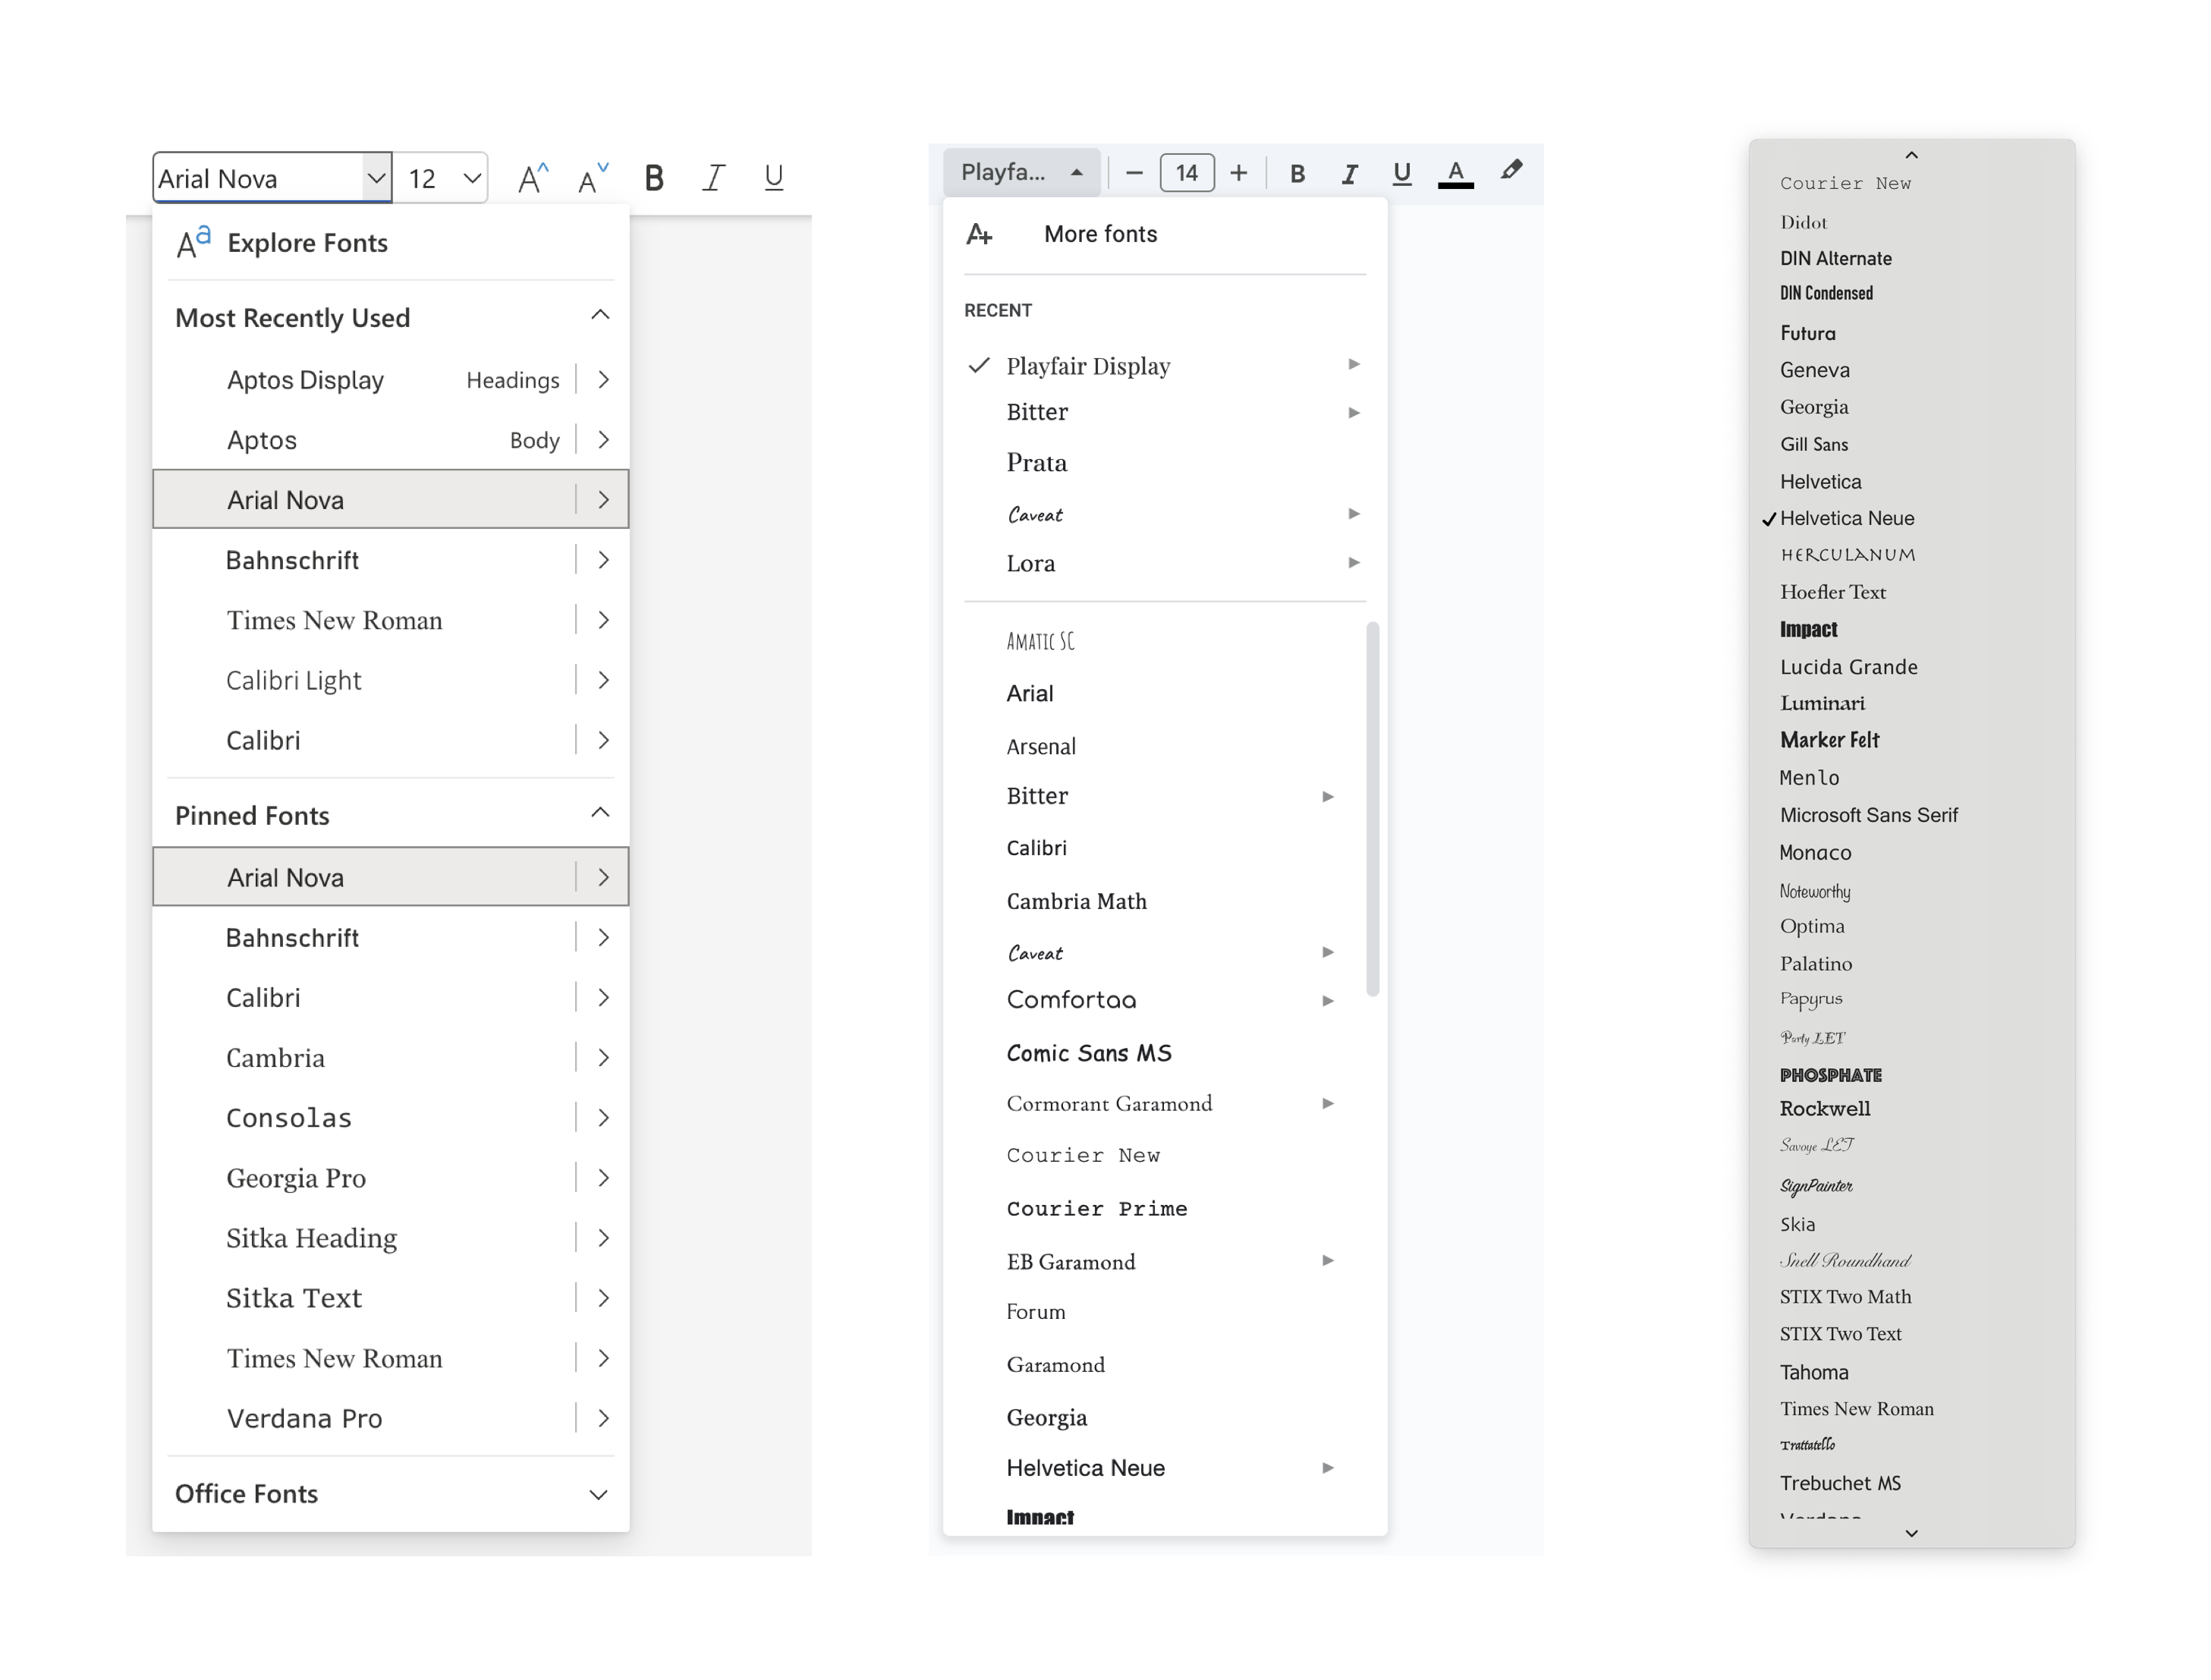
\includegraphics[width=1\textwidth]{images/font-selectors.png}
    \caption{Current font selection interfaces in Microsoft Word, Google Docs, and Apple Pages}
    \label{fig:font-selectors}
\end{figure}

\subsection{Font Selection Innovation} \label{font-selection-innovation}

There has been some limited progress, in recent years, in the field of font selection interfaces. Specifically, both Google Fonts and Canva, a popular online graphic design tool, have experimented with language-based font selection tools. Both of these interfaces break from the common list-based font selection tool, but both also have some significant drawbacks and flaws. This section will explore these two novel font selection interfaces and their respective contributions.

% own screenshots
\begin{figure}[H]
    \centering
    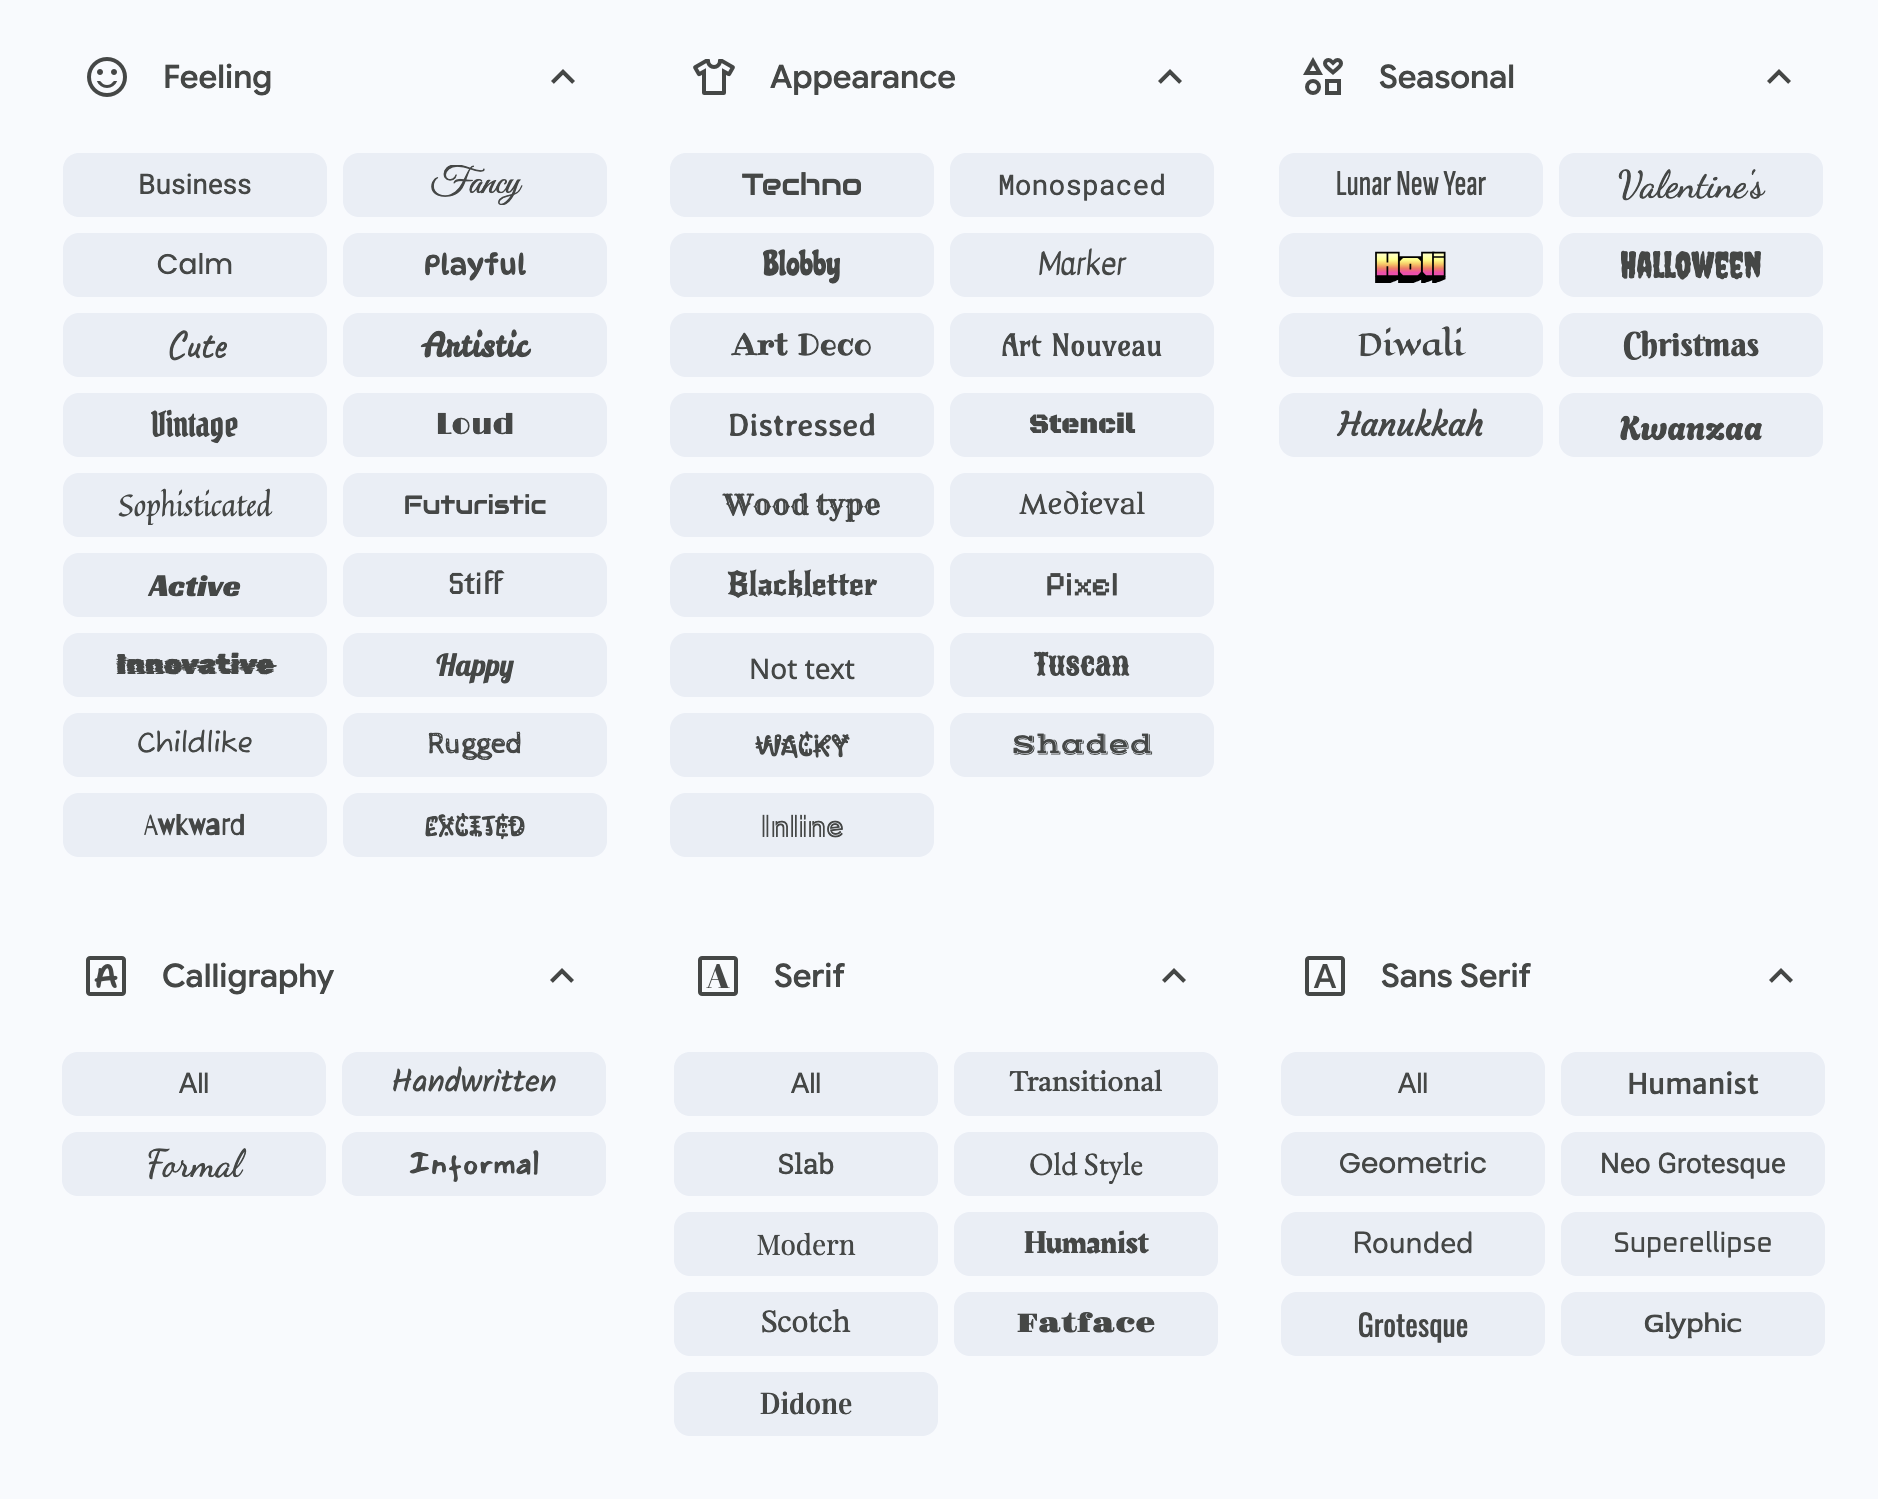
\includegraphics[width=.85\textwidth]{images/google-font-categories.png}
    \caption{Some typeface categorizations in the new Google Fonts interface}
    \label{fig:google-font-categories}
\end{figure}

The new font selection interface on the Google Fonts website\footnote{https://fonts.google.com} was released in early 2025. Whereas Google previously organized their fonts into 5 broad categories (Display, Handwriting, Monospace, Serif, and Sans Serif), their new interface introduces a much larger set of typeface categories, broken into broader parent categories (see Figure \ref{fig:google-font-categories}). In the ``Feeling" category, for example, users can filter ``Happy" fonts, ``Calm" or ``Playful" fonts, and ``Childlike" or ``Awkward" fonts. The new interface also includes appearance categories like ``Techno" or ``Art Deco," as well as holiday categories for Halloween, Hanukkah, Christmas, and Holi, among others.

% own screenshots
\begin{figure}
    \centering
    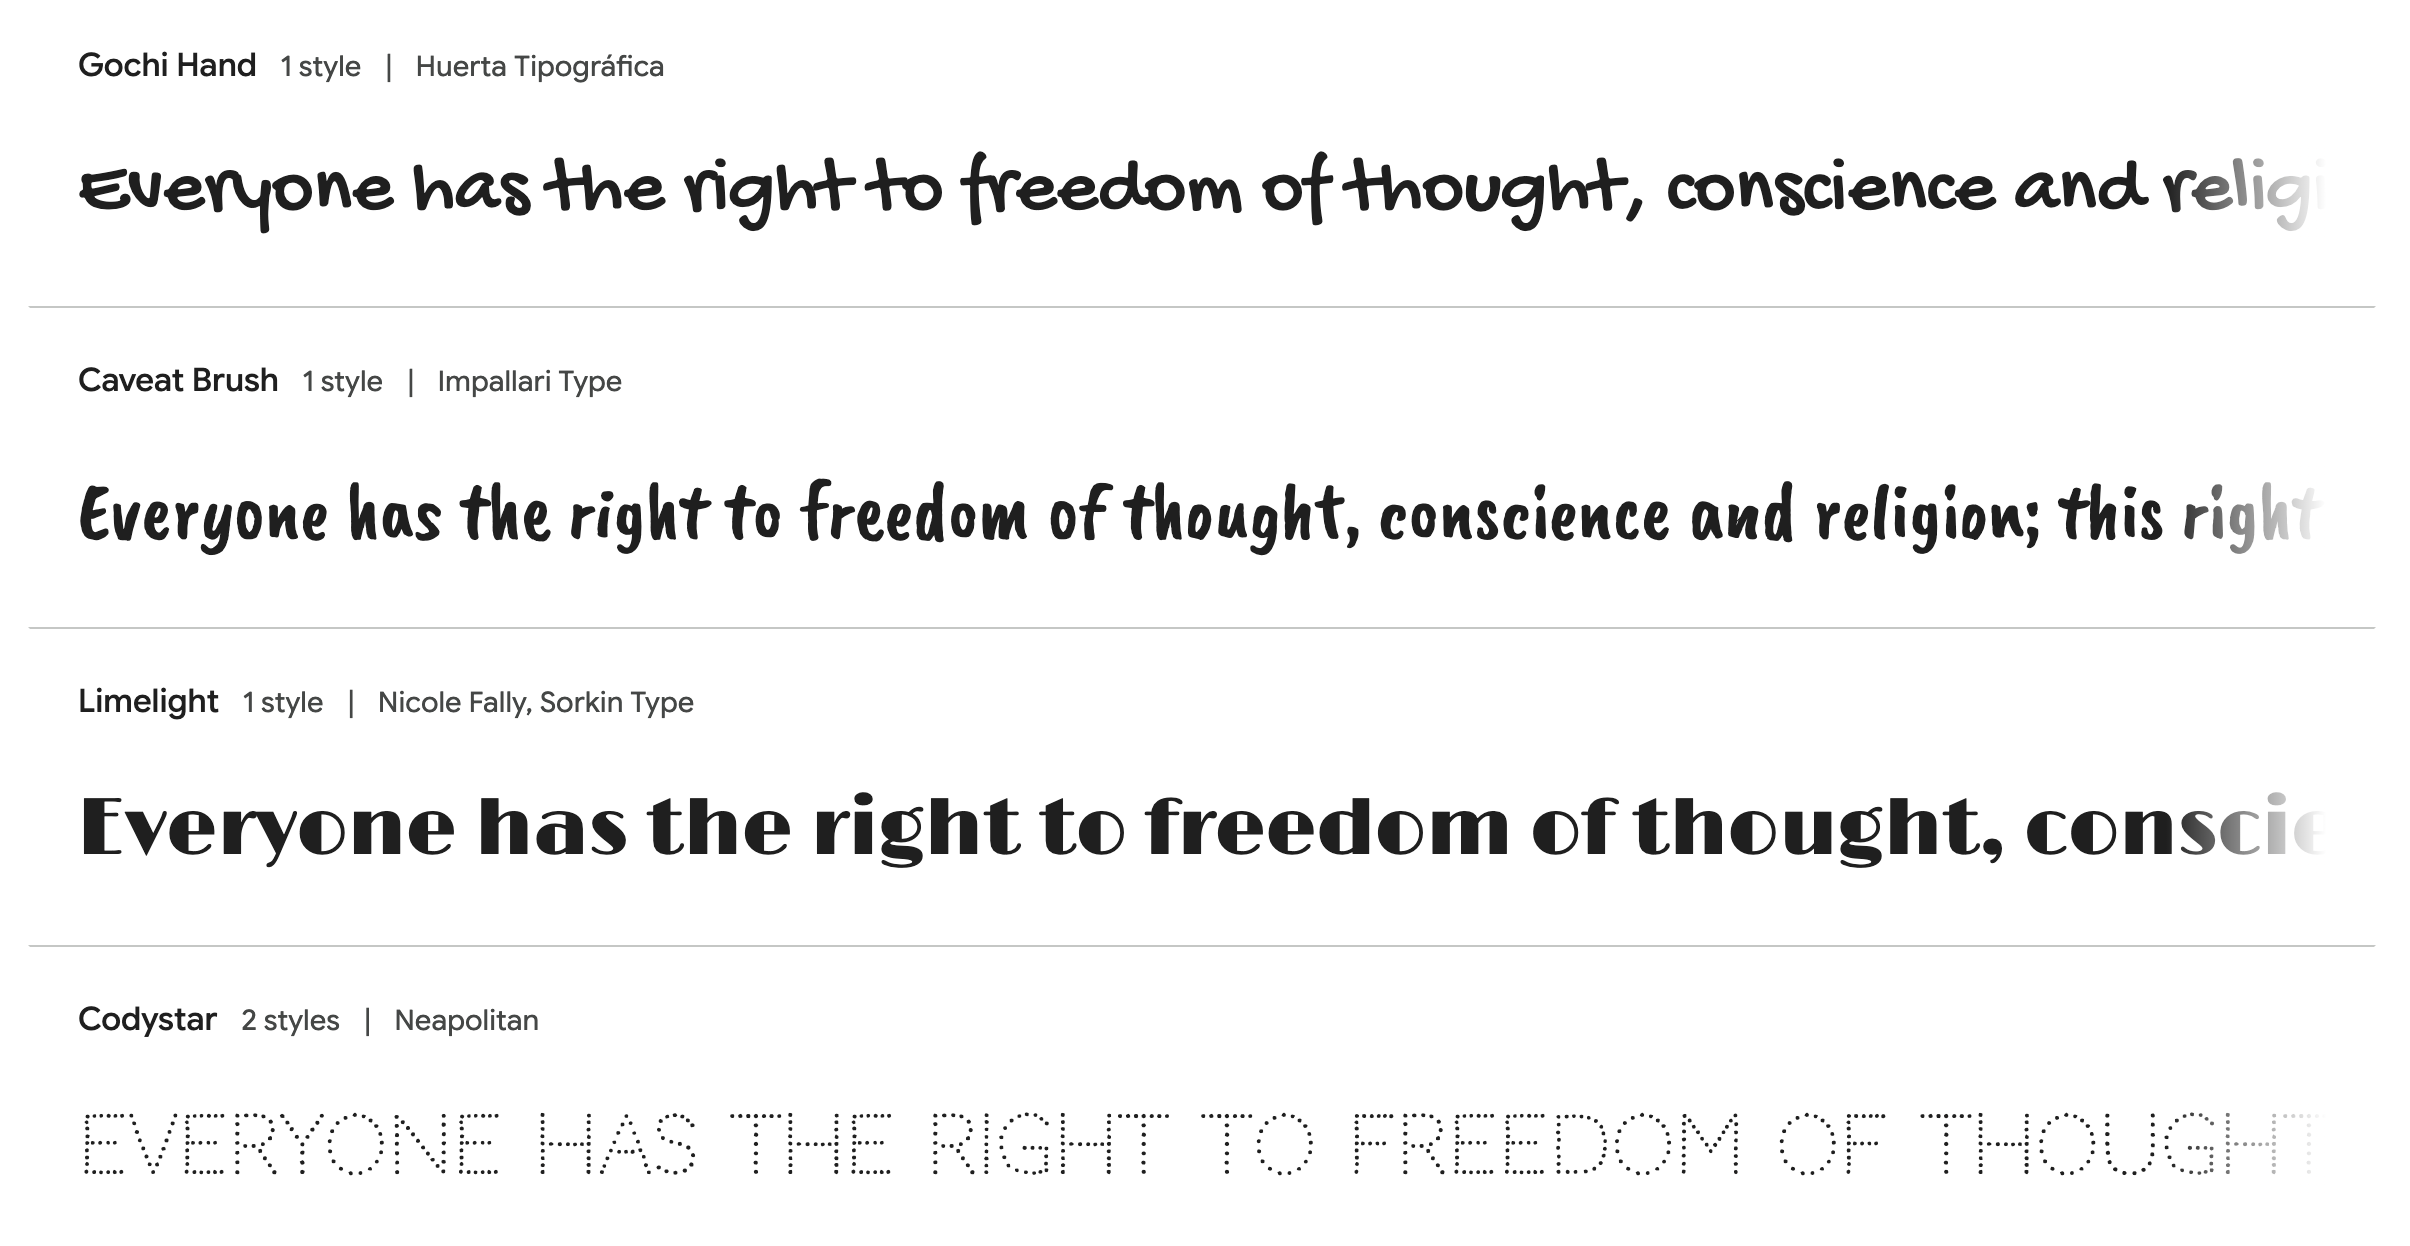
\includegraphics[width=1\textwidth]{images/google-fonts-christmas.png}
    \caption{Some of the ``Christmas'' fonts in Google Fonts do not seem very Christmassy}
    \label{fig:google-fonts-christmas}
\end{figure}

Google Font's categories break with the basic list-based interface; however, the tool has several drawbacks. For one, the user is forced to choose between discrete categories, rather than an open-ended text input, limiting their selection process to preconceived descriptors. Additionally, these categorizations are subjective; and while many of the groupings seem fairly accurate, some are questionable (such as the ``Christmas'' fonts in Figure \ref{fig:google-fonts-christmas}). Most importantly, Google has not incorporated this new font selection tool into their main Google Suite applications (Google Docs, Google Slides, and Google Sheets) where the majority of their users are choosing fonts. Most users are unfamiliar with the Google Fonts website, and therefore will not use the interface. This new font selector tool, available only from a separate website, is an interesting experiment in language-based font selection, but not yet more than that.

Canva, a popular online graphic design tool, has also experimented with a language-based font selection tool. Their main design interface allows users access to select fonts via a text input field. For example, a user could type ``Modern'' and they would be presented with a wide-variety of modern-style fonts. However, while the input prompt appears open-ended, the tool actually only works for a small set of keywords; for most text input, it will either yield no results or simply return fonts whose name contains that keyword (see Figure \ref{fig:canva-font-selector}). For many unseen inputs like ``Professional,'' ``Cheerful,'' ``Ancient,'' and ``Lightweight'' the tool returns no results at all.

% own screenshots
\begin{figure}
    \centering
    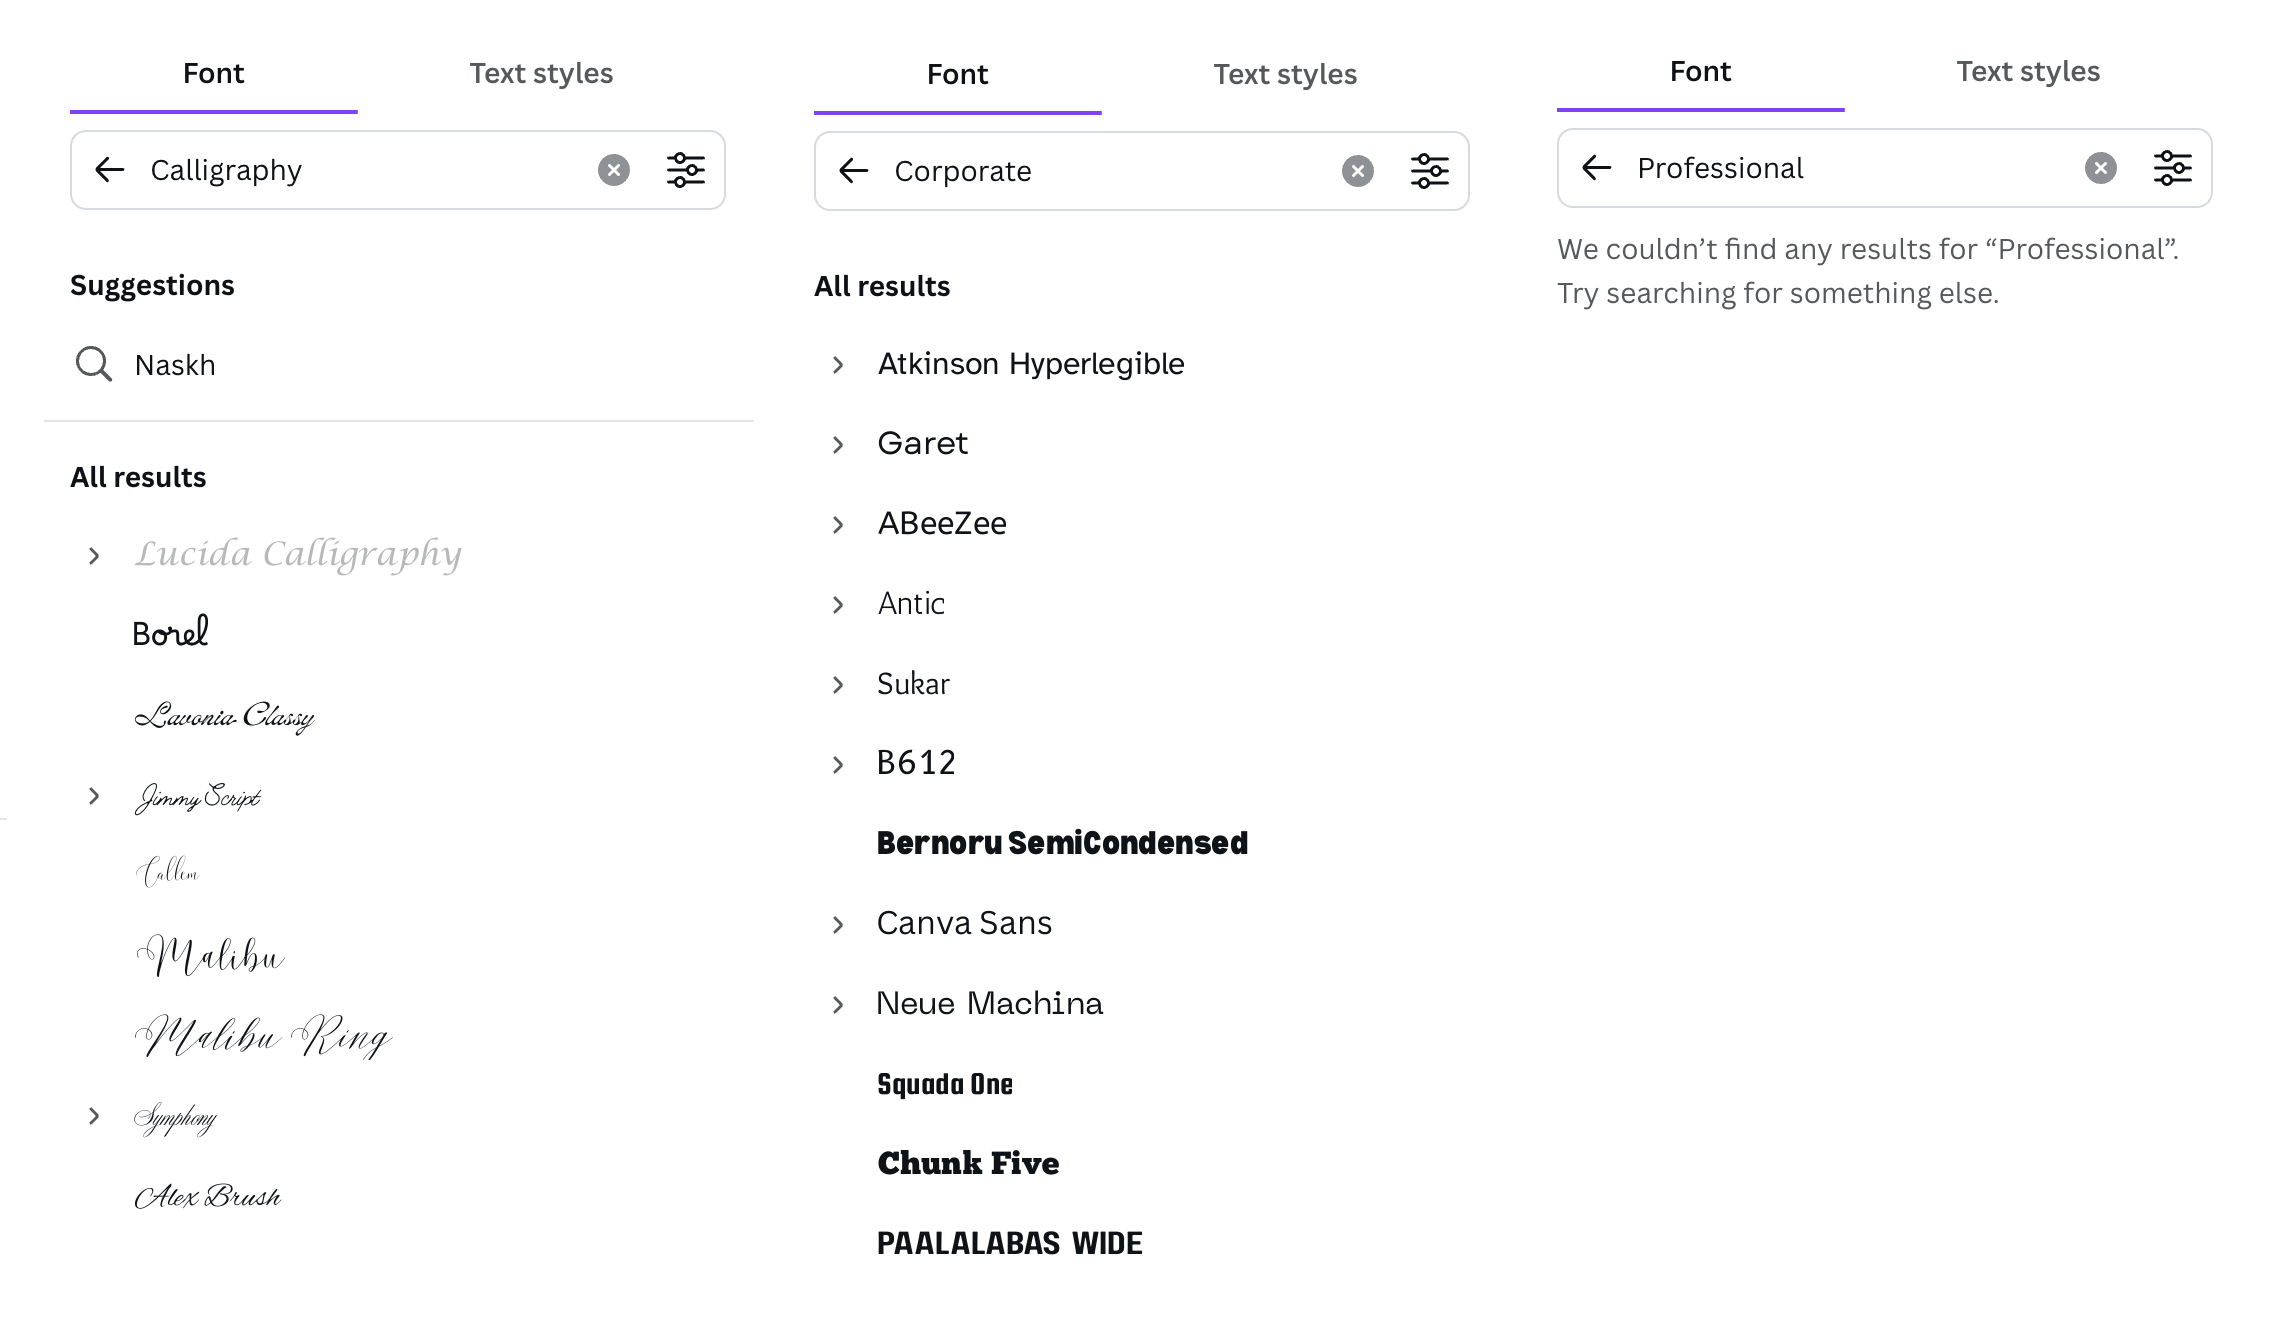
\includegraphics[width=.95\textwidth]{images/canva-font-selector.png}
    \caption{Example usages of the Canva text-based font selector tool}
    \label{fig:canva-font-selector}
\end{figure}

\subsection{Issues with Language-Based Font Selection}

Both of the above tools use keyword descriptors for font selection, one with predetermined style categories (Google Fonts) and the other with an open-ended search box which, in reality, allows only a limited set of keywords as input (Canva). The direction of this approach, however, is not a bad one. Language is one of the ways in which humans fundamentally conceive of the world, including with respect to visual style. Especially given the popularization of Large Language Models (LLMs) and chatbots, there is certainly an open space for innovation with language-based font selection. However, there are a couple key problems with creating these language-based font selection models. First of all, visual style is quite subjective: one user might find a certain font ``wacky'' while another might find that font ``sad'' or ``disgusting.'' A font which one user finds ``professional'' another might find ``playful.'' Building a language-based model for font selection should therefore account for user subjectivity in its recommendations. Secondly, there is a relative lack of datasets which connect typefaces to language-based style characteristics. Shaikh et al.\ \cite{shaikh2006} perform an online study with hundreds of participants to generate a dataset of only 20 fonts and 15 style adjectives. O'Donovan et al.\ \cite{odonovan2014} generate a larger dataset of 200 fonts and 31 style adjectives, but this is still relatively small when compared with the hundreds of thousands of available fonts and the many possible dimensions of style. For this project, we mostly avoid the issue of language-based font selection, and rather focus on the use of unsupervised neural models in building useful style-based font selection tools.

% from rgbacolorpicker.com
\begin{figure}[p]
    \centering
    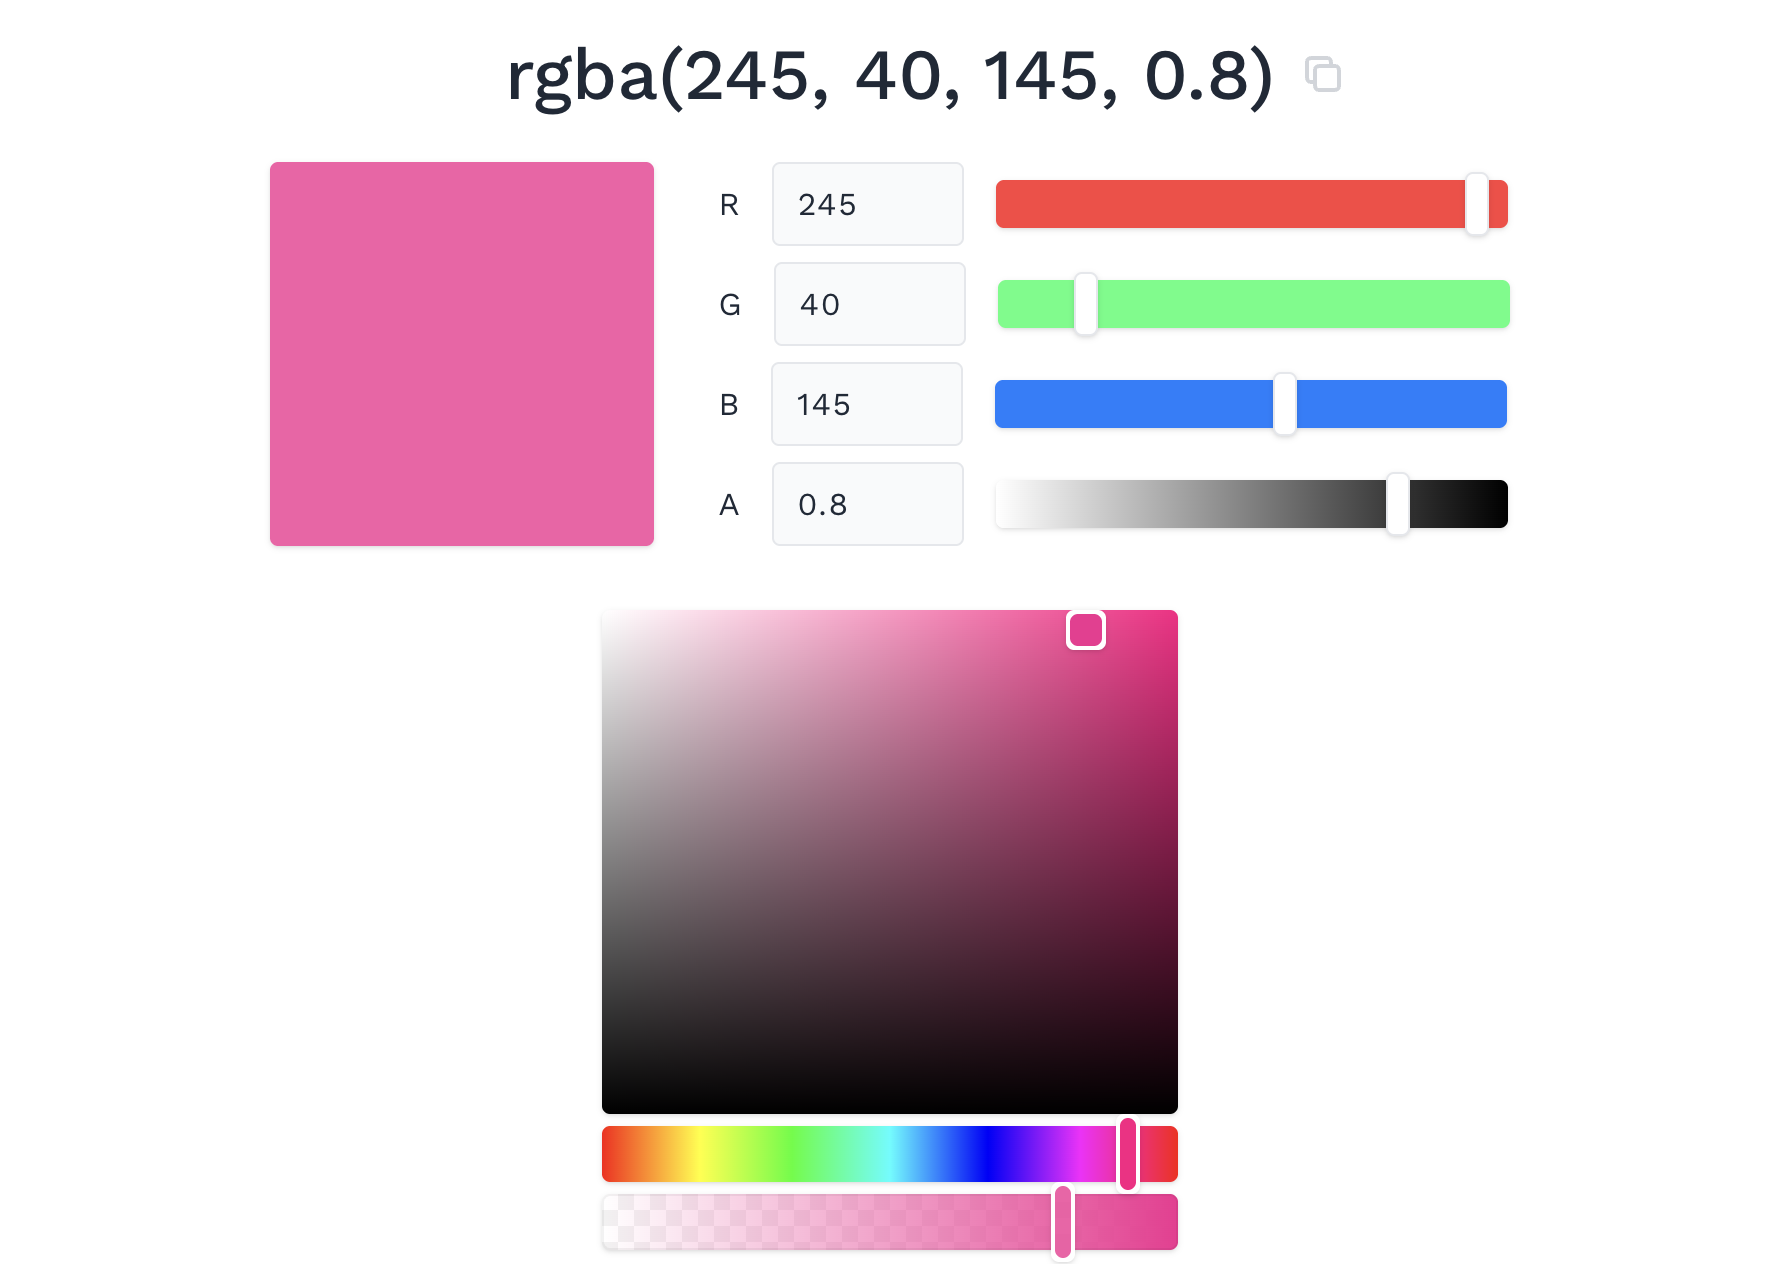
\includegraphics[width=0.8\textwidth]{images/basic-color-picker.png}
    \caption{A basic color selection interface with gradient, numeric, and slider controls}
    \label{fig:basic-color-picker}
\end{figure}

% from color.adobe.com
\begin{figure}[p]
    \centering
    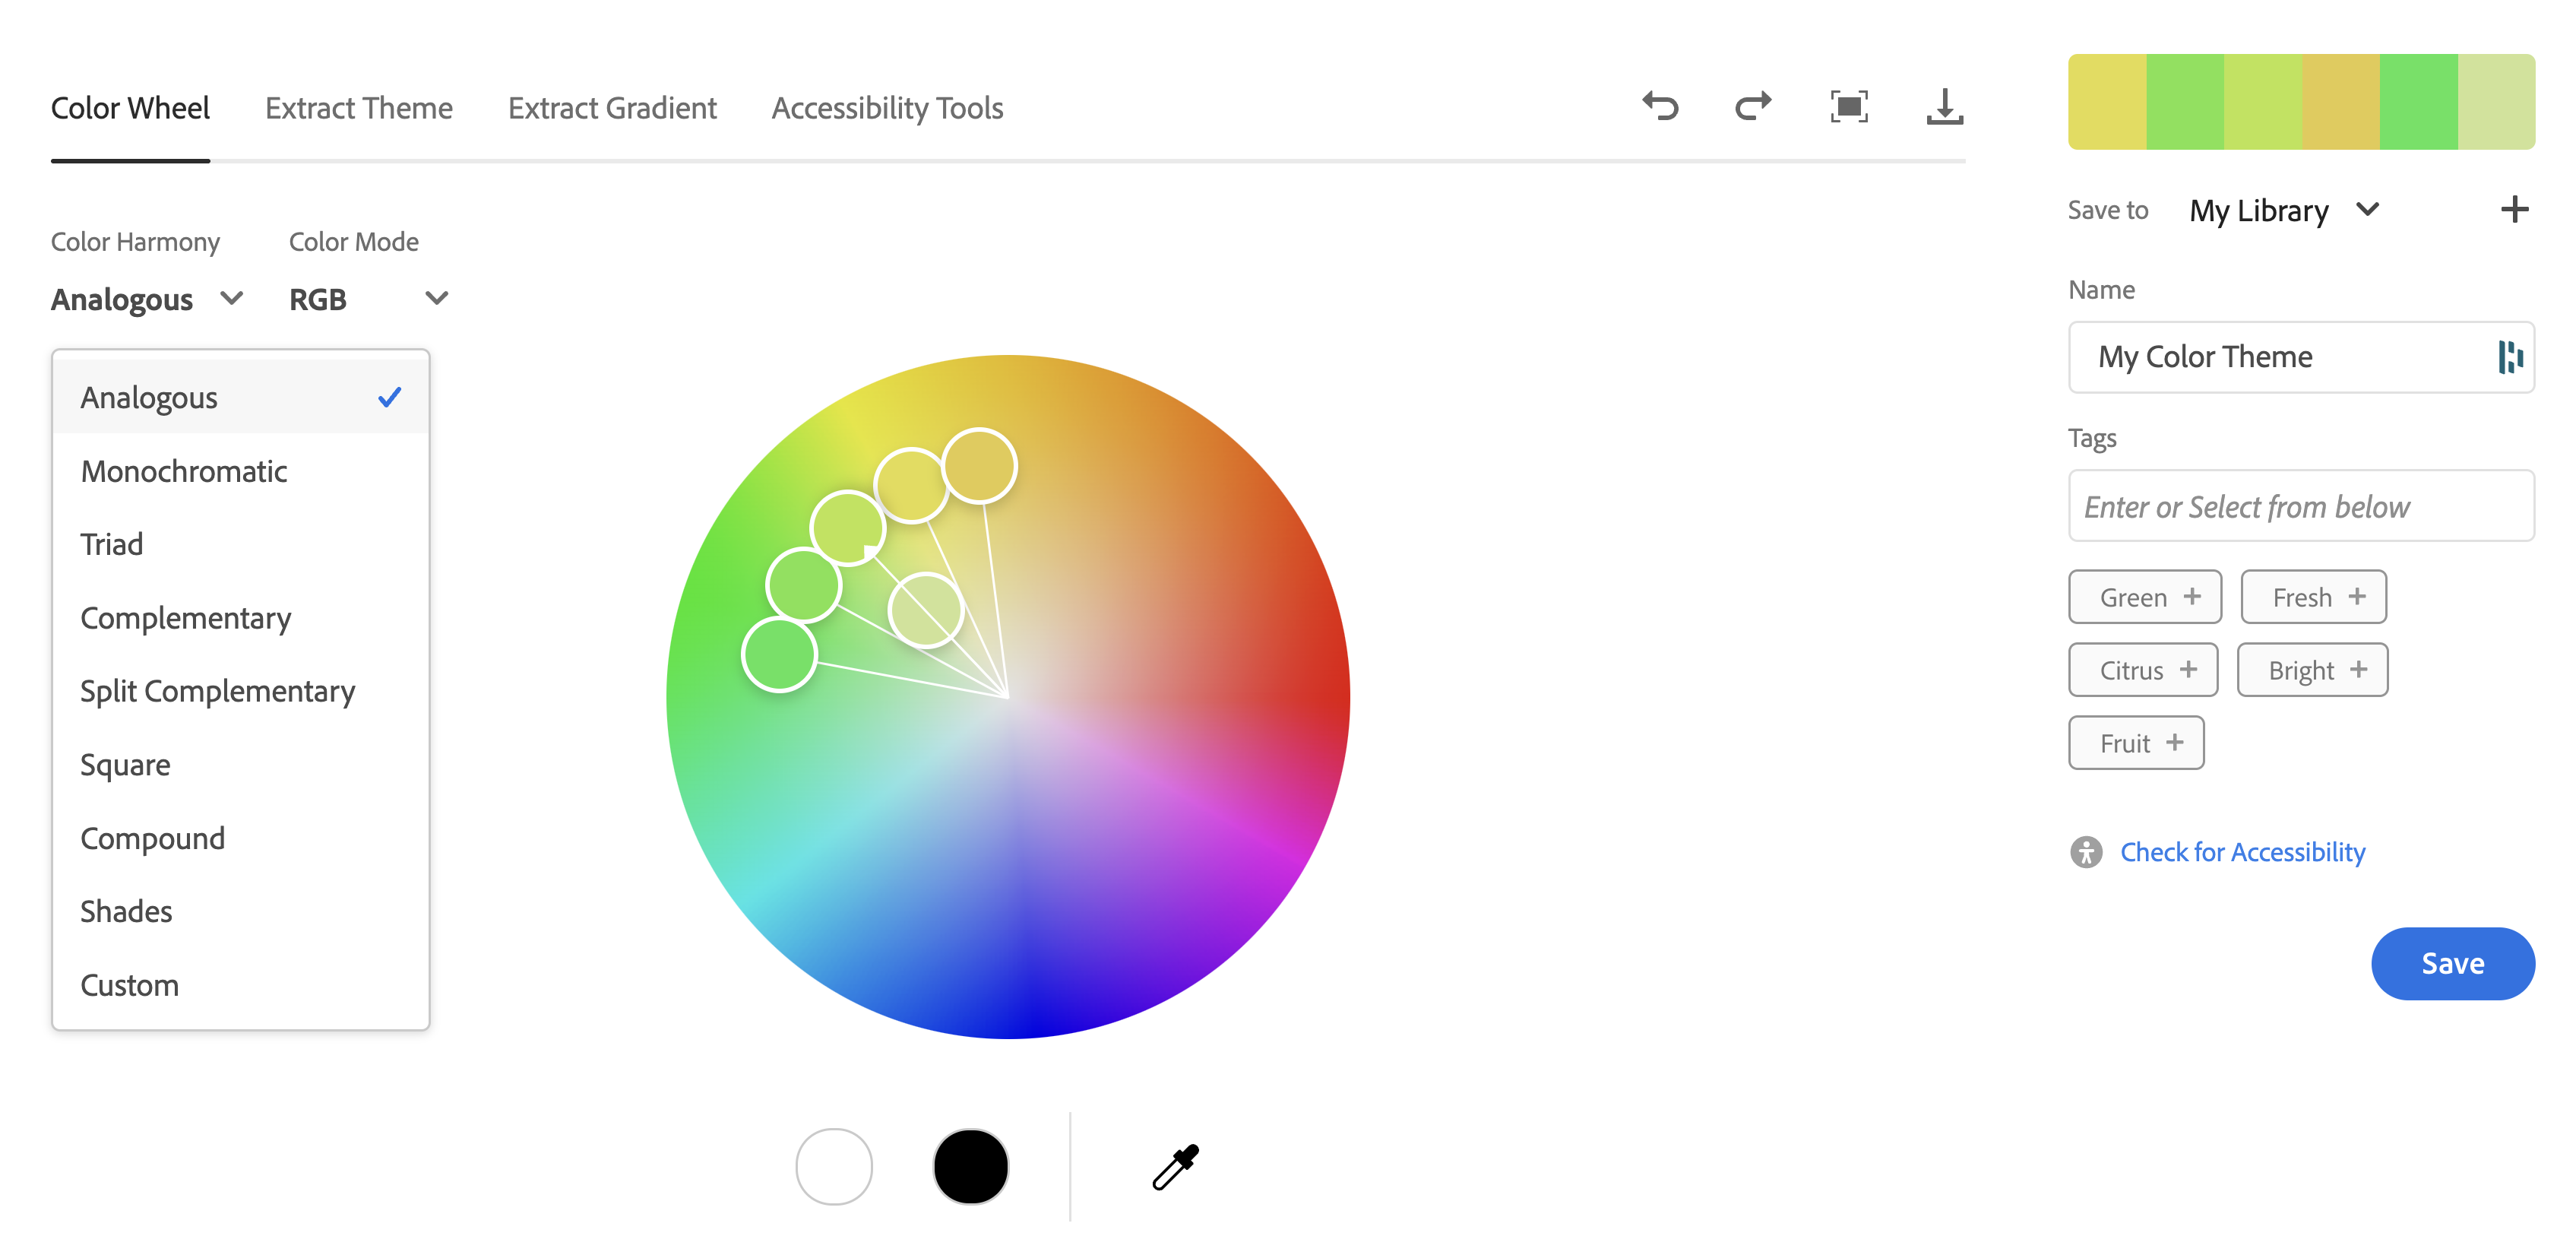
\includegraphics[width=\textwidth]{images/adobe-color.png}
    \caption{Adobe Color selection interface, with a color wheel, multiple color bases, color harmony-based selection, and the ability to save colors}
    \label{fig:adobe-color}
\end{figure}

\subsection{An Analogue: Color Selection}

A useful analogue when considering the issue of typeface selection is another common problem in graphic design: color selection. The field of color selection has produced a much wider range of selection interfaces, which suggests a potential for a much more diverse set of font selection tools. Figure \ref{fig:basic-color-picker} shows a common, basic color selection tool containing several ways to interact with its many available colors: sliders, numeric input, and a 2-dimensional gradient. Color can be represented using a 4-dimensional basis called RGBA: red-value, green-value, blue-value, and transparency-value. The first three are based on a hexadecimal scale, allowing values between 0 and 255, while the transparency value is constrained between 0 and 1. By representing color using a multi-dimensional basis, users have an intuitive, finer-grained control over the color selection process. This is more useful than, say, selecting from an alphabetized list of colors (Apricot, Aquamarine, Baby Blue, Canary Yellow...), which---similar to an alphabetized list of fonts---does not provide users with a very meaningful way to navigate the dimensions of color. There are many other popular tools for color selection: Adobe Color, for example, utilizes a popular color-wheel tool, and additionally includes features to change color basis (CMYK and RGBA are the most common color bases, but other more obscure ones exist), pick a set of colors based on a particular harmony (Monochromatic, Triad, Complementary, e.g.), and save colors to a library for later access (see Figure \ref{fig:adobe-color}).

The wide range of diverse color selection interfaces and color bases suggests a potential for similarly-diverse, useful selection tools for typeface which provide control over the many dimensions of typeface style. While typefaces and their style cannot be decomposed as easily as color, their style \emph{can} be represented using a vector basis---as we will show in subsequent chapters---and building selection tools on a vector space of style dimensions could allow users greater control in typeface selection---similar to the level of control users have in color selection. Imagine, perhaps, a gradient of fonts, or sliders which control different aspects of font style. These ideas are not farfetched: as our research will show, neural networks---specifically autoencoder-like neural network models---can be used to distill quantitative style encodings from font image data, which provides a foundation upon which to build better style-based font selection tools.

\section{Autoencoders}

As previously stated, we hypothesize that neural networks might provide a useful foundation for font selection tools by generating typeface style encodings. More specifically, we focus on autoencoder and autoencoder-like models in our neural network design. This section provides background on the autoencoder model and why autoencoder-like neural networks might provide a useful foundation for creating style-based font selection tools.

\subsection{Autoencoder Model}

The autoencoder \cite{rumelhart1986} is a specific type of neural network trained to exactly reconstruct its input. The model is composed of two parts: an encoder, which transforms the input to an intermediate representation (usually smaller than the input representation) through a series of linear and nonlinear operations; and the decoder, which transforms the intermediate representation back to the original input size. By minimizing the loss of this neural network during training, the encoder learns to condense the input data for later reconstruction, and the decoder learns to reconstruct that data based on the intermediate representation generated by the encoder.

% from Bank et al. "Autoencoders" DO I NEED TO CITE THIS?
\begin{figure}[h]
    \centering
    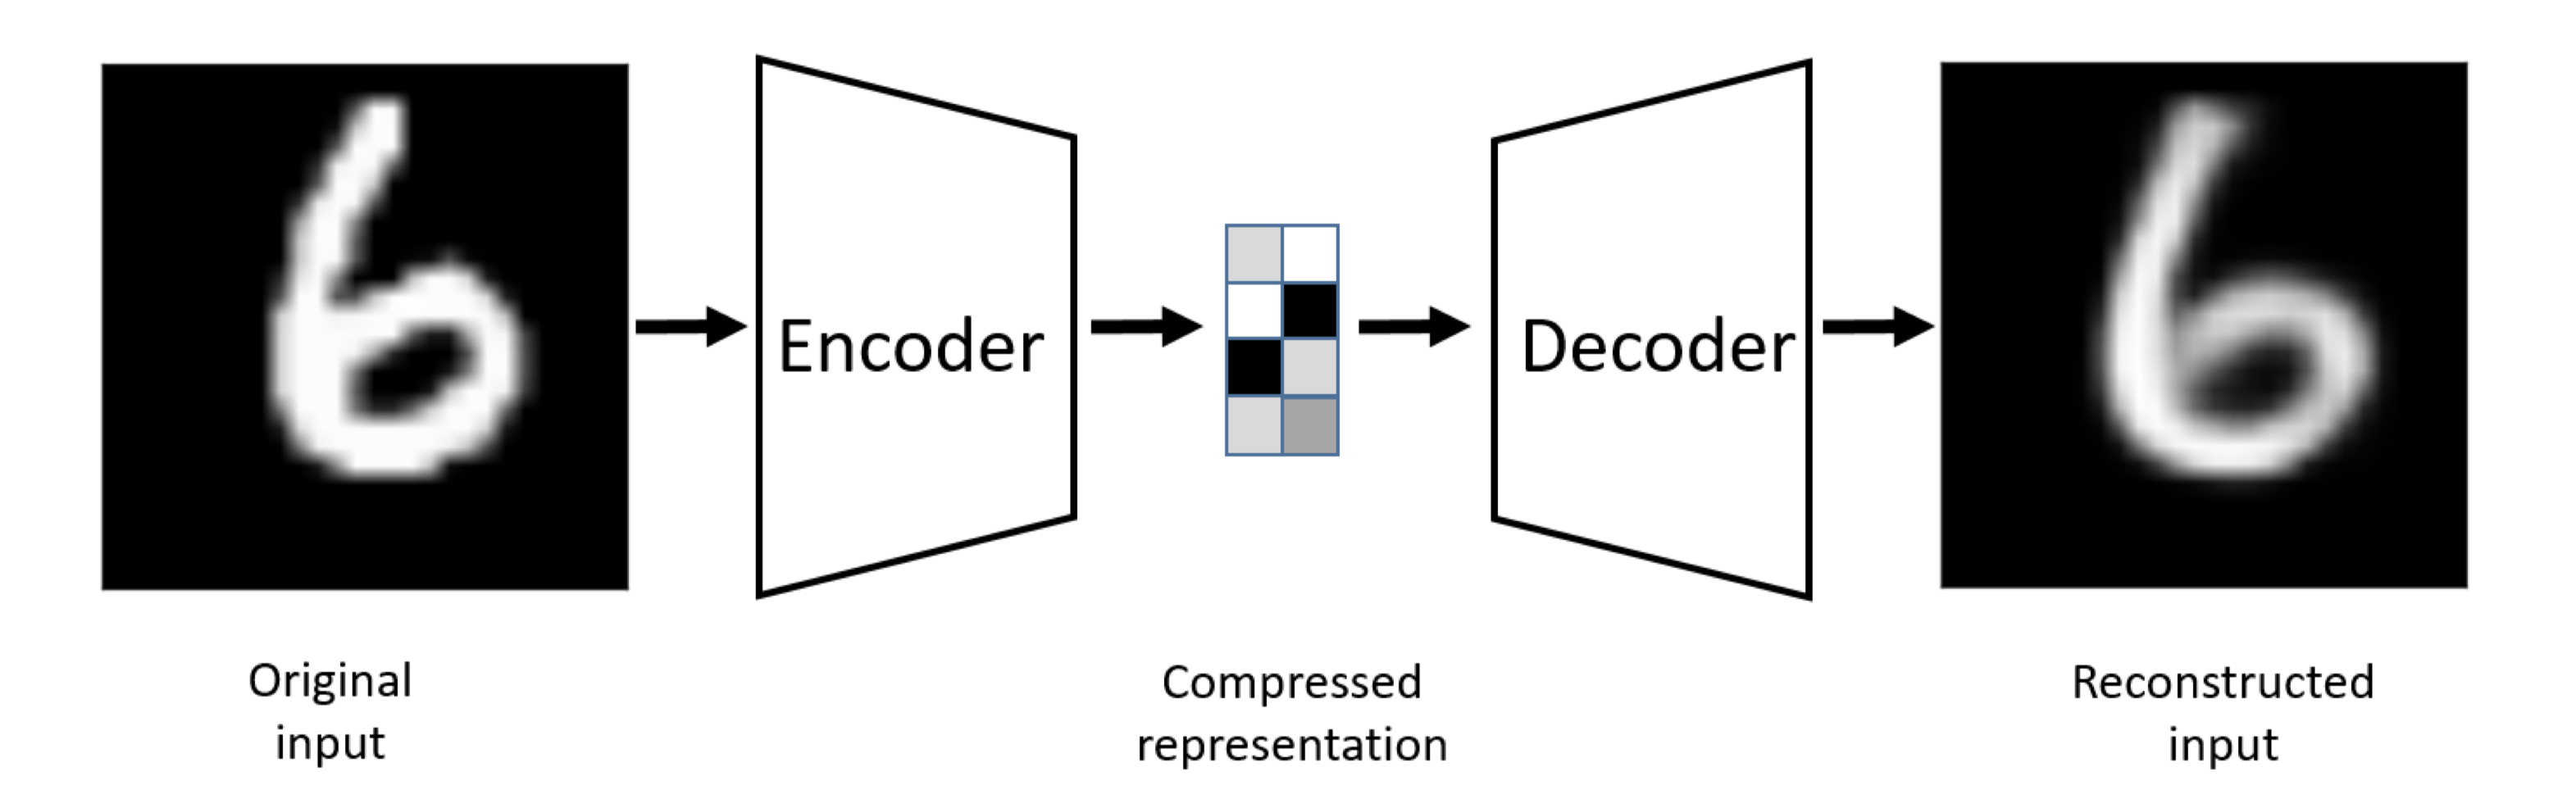
\includegraphics[width=\textwidth]{images/autoencoder-model.png}
    \caption{Basic autoencoder model applied on an image from MNIST, a dataset of handwritten images widely-used for image classification tasks \cite{lecun1998}}
    \label{fig:autoencoder-model}
\end{figure}

The autoencoder model may seem of little use---why would we want to reconstruct data which we already have? The main goal of an autoencoder, however, is not the final reconstructed output but rather the intermediate representation---which distills the essentials of the input. In order for the decoder to be able to accurately reconstruct input data which it has never seen, the encoder part of the model must encode an intermediate encoding that captures enough salient aspects of the input for the reconstruction stage. Thus, the autoencoder's intermediate representation tends to be a rich and concise summary of the input. In our research, we leverage these encodings as a proxy for typeface style. Bank et al.\ \cite{bank2021autoencoders} write:

\begin{quote}
    ...the goal of autoencoders is to get a compressed and meaningful
    representation. We would like to have a representation that is meaningful to us...
\end{quote}

In order to create meaningful representations, however, some steps must be taken to avoid simply learning the identity function. To accomplish this, the autoencoder model usually includes a bottleneck---meaning that the encoder must compress the input before giving it to the decoder (see Figure \ref{fig:autoencoder-model}). Therefore, the model \emph{cannot} simply learn the identity function and must learn to produce a useful, condensed version of the input. In our case, the purpose of training an autoencoder model to reconstruct font data is not the output images, but rather these intermediate encodings. Importantly, while a bottleneck is the most common technique to achieve this effect, other methods such as adding Gaussian noise \cite{bank2021autoencoders} can be used instead of or in addition to a bottleneck.

\subsection{Variations on the Autoencoder}

There have been many variations on this basic autoencoder model \cite{michelucci2022}. While the basic autoencoder is unsupervised, it is possible to feed additional data into the autoencoder, such as data labels, in order to coerce the model to ignore these aspects of the input data in the construction of an intermediate representation. (In our research, we employ this method to disentangle \textit{content}---i.e. the character being represented---from \textit{style.}) Another alteration of the original autoencoder is the variational autoencoder (VAE) model \cite{kingma2013}, which uses probabilistic distributions to improve autoencoder performance, especially with respect to generative tasks. Rather than encoding an explicit intermediate encoding, VAEs encode the parameters of a multi-dimensional Gaussian distribution which represents the probabilistic space of the intermediate encoding. The decoder then samples randomly from the distribution and proceeds with the decoding task. This probabilistic model is especially useful in generative tasks, when the goal is to generate new content (e.g. to generate a new character in a font); but the continuous latent space encoded by VAEs can also be directly used, as in our case, as a compact representation of salient input properties like visual style.

\section{Previous Work}

There has been previous scholarly work on improving font selection interfaces, especially based around font inference models. This section explores some of these models, one based on crowdsourced data, and the others on neural inference models. Both of these approaches have informed our research, but the neural inference models have particularly influenced the models we implemented. Particularly, we adapt the Srivatsan et al.\ model \cite{srivatsan2020} in our work and use the style encodings trained by the model to build our typeface selector tool.

% own screenshots
\begin{figure}
    \centering
    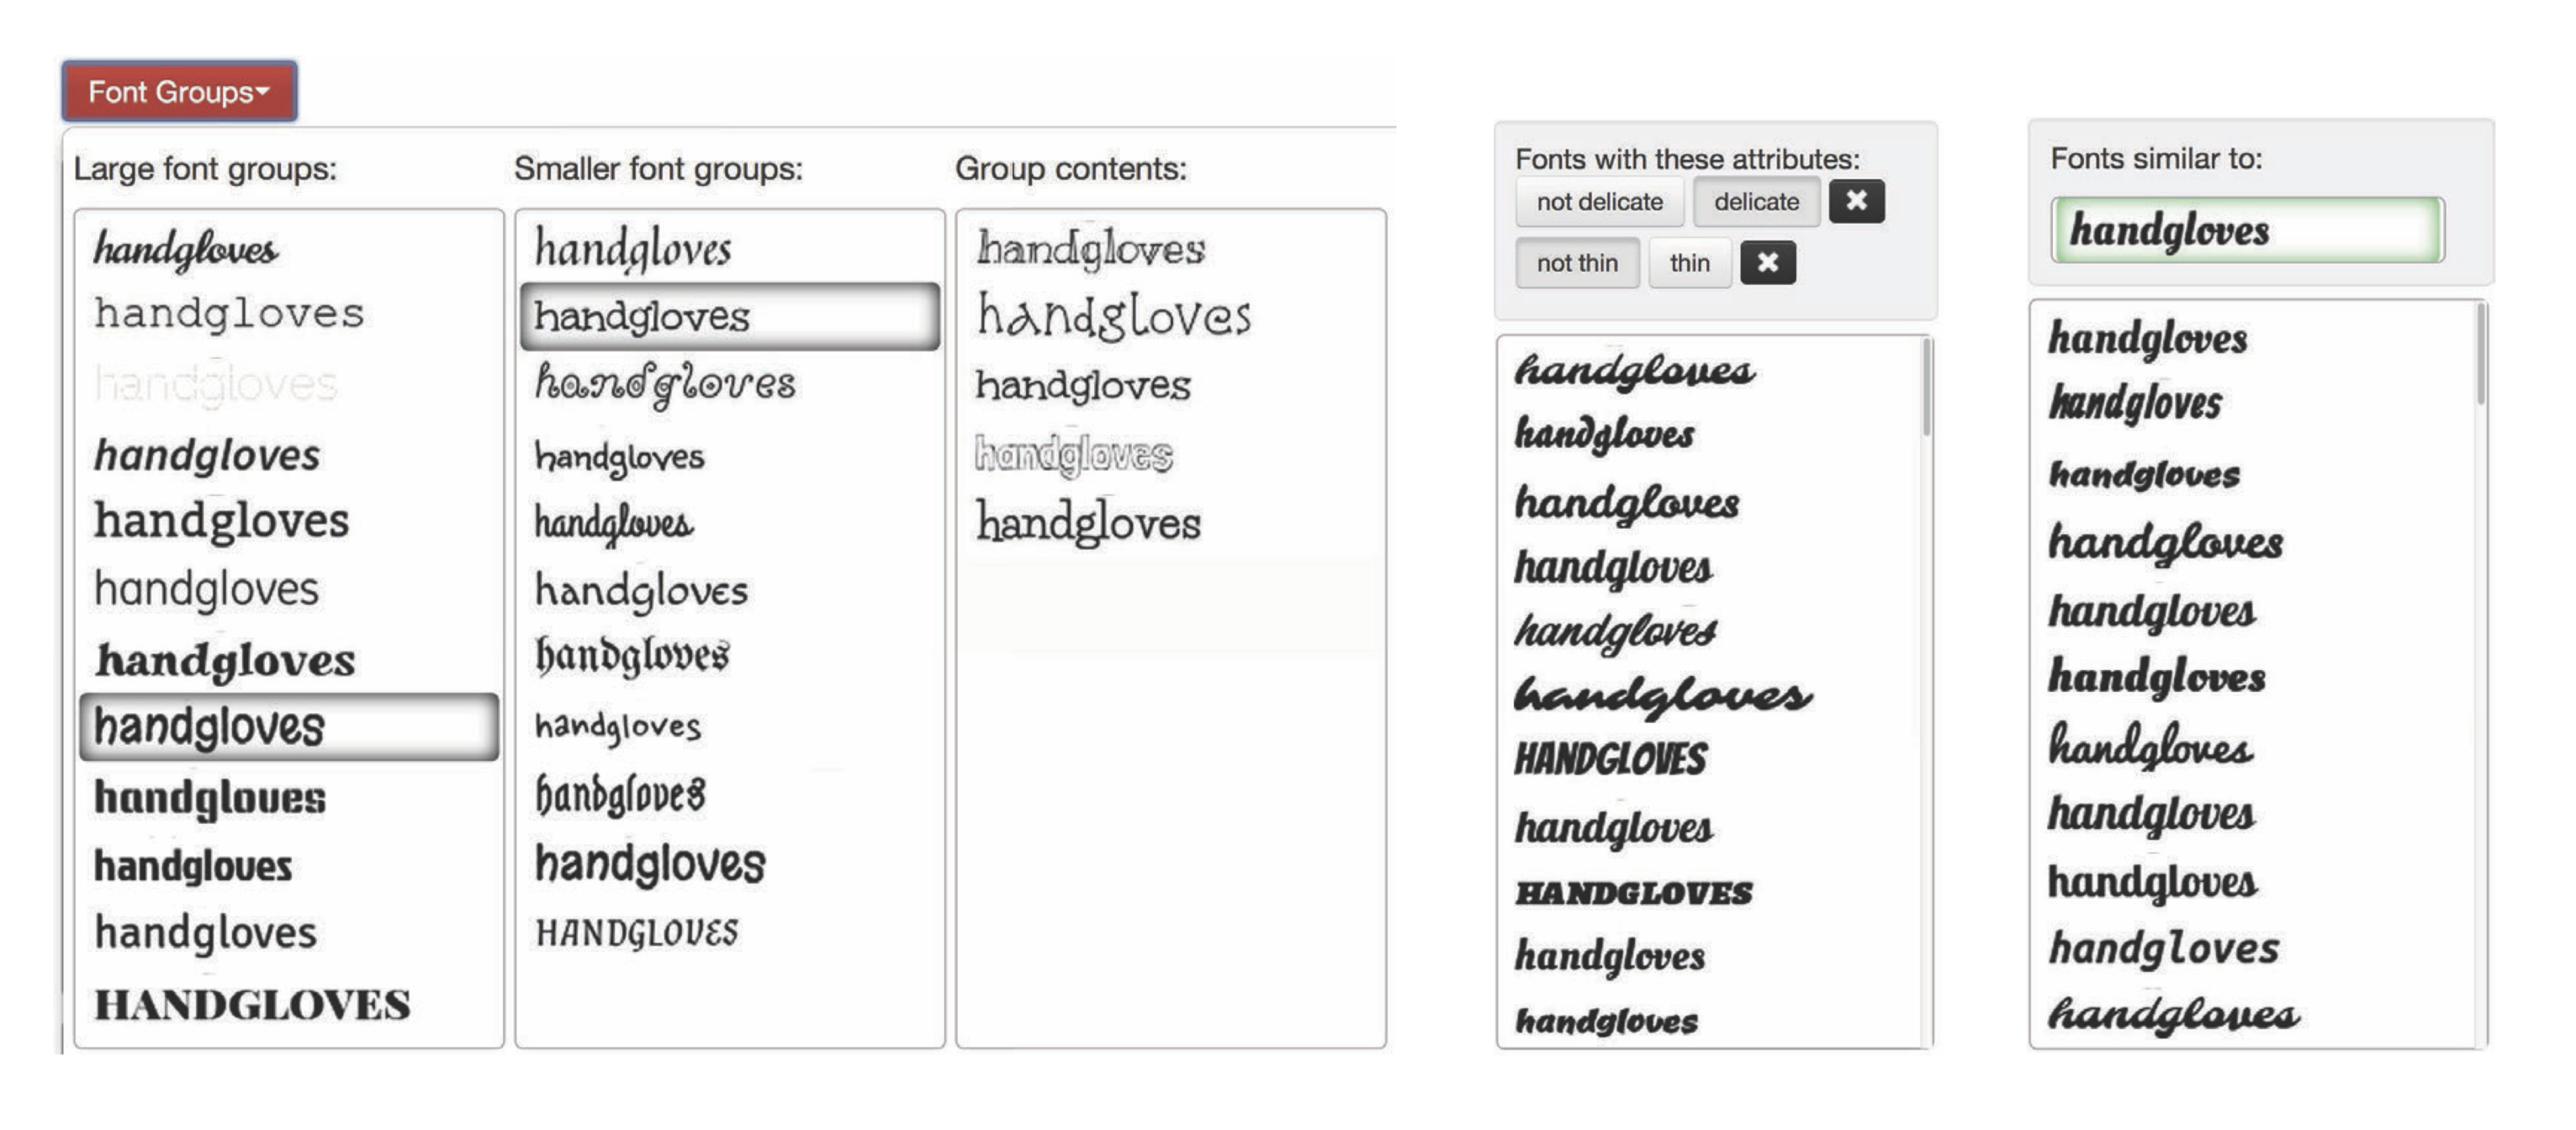
\includegraphics[width=1\textwidth]{images/odonovan-interfaces.png}
    \caption{Group Interface, Attribute Interface, and Search-By-Similarity selection tools from O'Donovan et al.\ \cite{odonovan2014}}
    \label{fig:odonovan-interfaces}
\end{figure}

\subsection{Crowdsourced Models}

O'Donovan et al.\ \cite{odonovan2014} proposes three novel font-selection interfaces, built on crowdsourced data from Amazon Mechanical Turk (MTurk): one based around verbal attributes such as ``formal,'' ``friendly,'' or ``legible'' called Attribute Interface; another which clusters fonts hierarchically based on visual similarity, called Group Interface; and a third, to be paired with the other two methods, which provides users with a list of similar fonts to the current selection, called Search-By-Similarity (see Figure \ref{fig:odonovan-interfaces}). The researchers built these models on crowdsourced data collected through MTurk: they prompted users to answer questions such as ``Which of these two fonts is more strong?'' or ``Which of these fonts is more silly?'' to collect attribute data, and asked questions like ``Which of these two fonts—Font B or Font C—is more similar to Font A?'' in order to build similarity data. The Group Interface model splits fonts into large categories based on similarity, creating a tree-like font selection tool where users can progressively narrow down their font selection task. The Attribute Interface, similar to the Google Fonts and Canva interfaces, attaches adjective descriptors to fonts, which is helpful as humans tend to conceptualize style based on verbal descriptors. Finally, they use the similarity data to create their Search-By-Similarity tool, to be used in conjunction with the other two methods: given a selected font, which fonts are most similar according to other users? This provides an important principle for typeface selection: if a user is looking to select a font based on style characteristics, it is useful to see other fonts that are similar according to other users. All of these tools are potentially useful ways to navigate typeface selection by means of style, but it should be noted that basing these attributes and similarity scores on crowdsourced data means that these tools may not align with every user's subjective sense of style. O'Donovan et al.\ additionally conducted user studies, also on MTurk, presenting users with either font matching or design tasks to evaluate their interfaces against a baseline font selector tool. The researchers found positive results for their novel font selection tools: participants were three times more likely to succeed in a font-matching task using any of the three proposed interfaces compared with a basic list-based interface, and they also found a small statistically significant improvement in user performance on the design task between their selection interfaces and the baseline.

\subsection{Inference Models}

There has also been some effort to build inference models around font character images, sometimes with the explicit purpose of building better user-interface for font selection. Cho et al.\ \cite{cho2022}, for example, builds a model with the explicit goal of generating latent space encodings of glyphs which are easily differentiable based on their font. They describe their model design as such:

\begin{quote}
    For the discriminative representation of a font from others, we propose a paired-glyph matching-based font representation learning model that attracts the representations of glyphs in the same font to one another, but pushes away those of other fonts.
\end{quote}

\begin{figure}
    \centering
    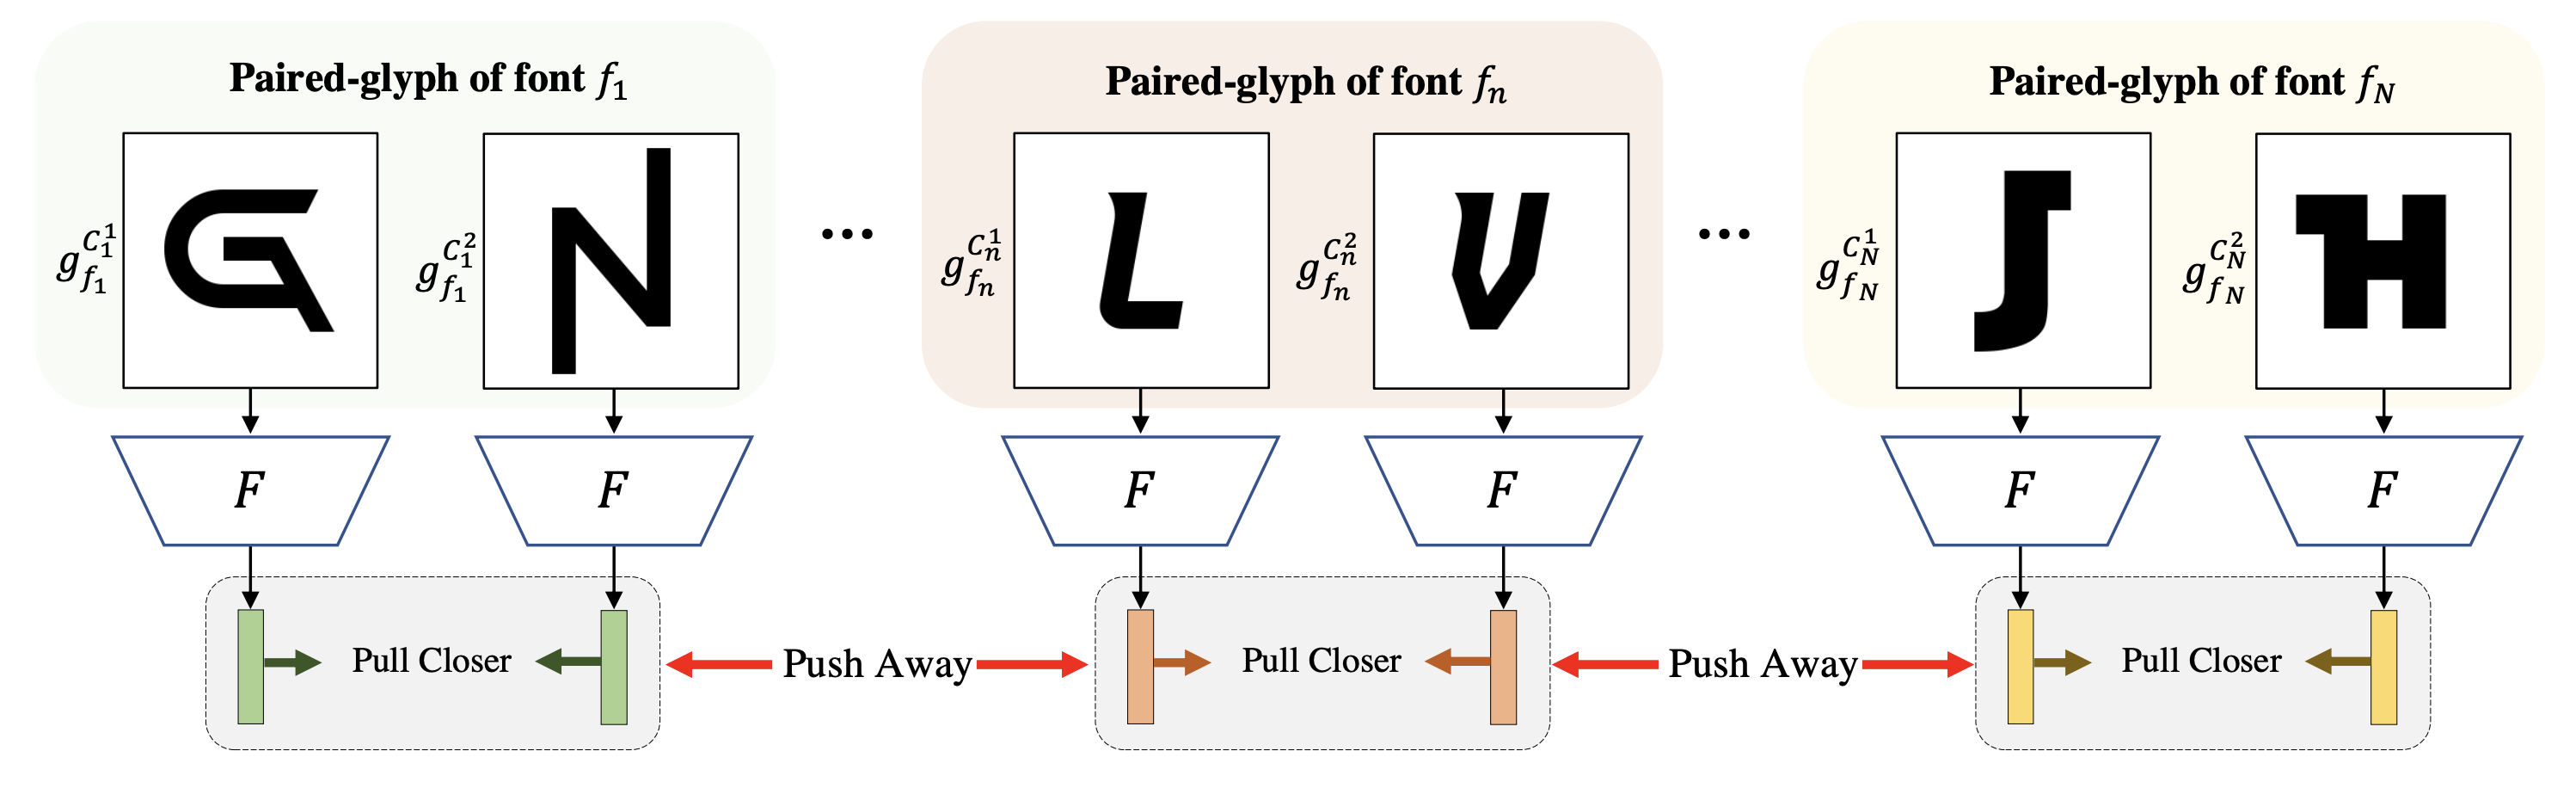
\includegraphics[width=1\textwidth]{images/cho-paired-glyph.png}
    \caption{Paired-glyph matching in Cho et al.\ \cite{cho2022}}
    \label{fig:cho-paired-glyph}
\end{figure}

Their paired-glyph matching, shown in Figure \ref{fig:cho-paired-glyph}, involves selecting random pairs of glyphs and training the model to prefer a low cosine similarity (more similar) between the representations if the glyphs are characters in the same font, and a high cosine similarity (less similar) if the glyphs come from different fonts. While Cho et al.\ succeeds in their goal of clustering the latent space representations of glyphs by typeface, it is unclear how well these encodings represent the stylistic aspects of typeface. Notably, the training technique focuses on decreasing the cosine similarity of encodings for characters of different typefaces, but it does not seem to have a mechanism to actually consider the style of a character or typeface. Rather, the training data for their model is essentially the \emph{name} of a font. As Figure \ref{fig:cho-latent-space} shows, their model performs well at discriminating character style encodings based on font---their model effectively clusters characters according to their typeface, denoted by point color---but the model space may not represent meaningful dimensions of typeface style (weight, size, serif) beyond simply separating fonts which are not identical.

\begin{figure}[]
    \centering
    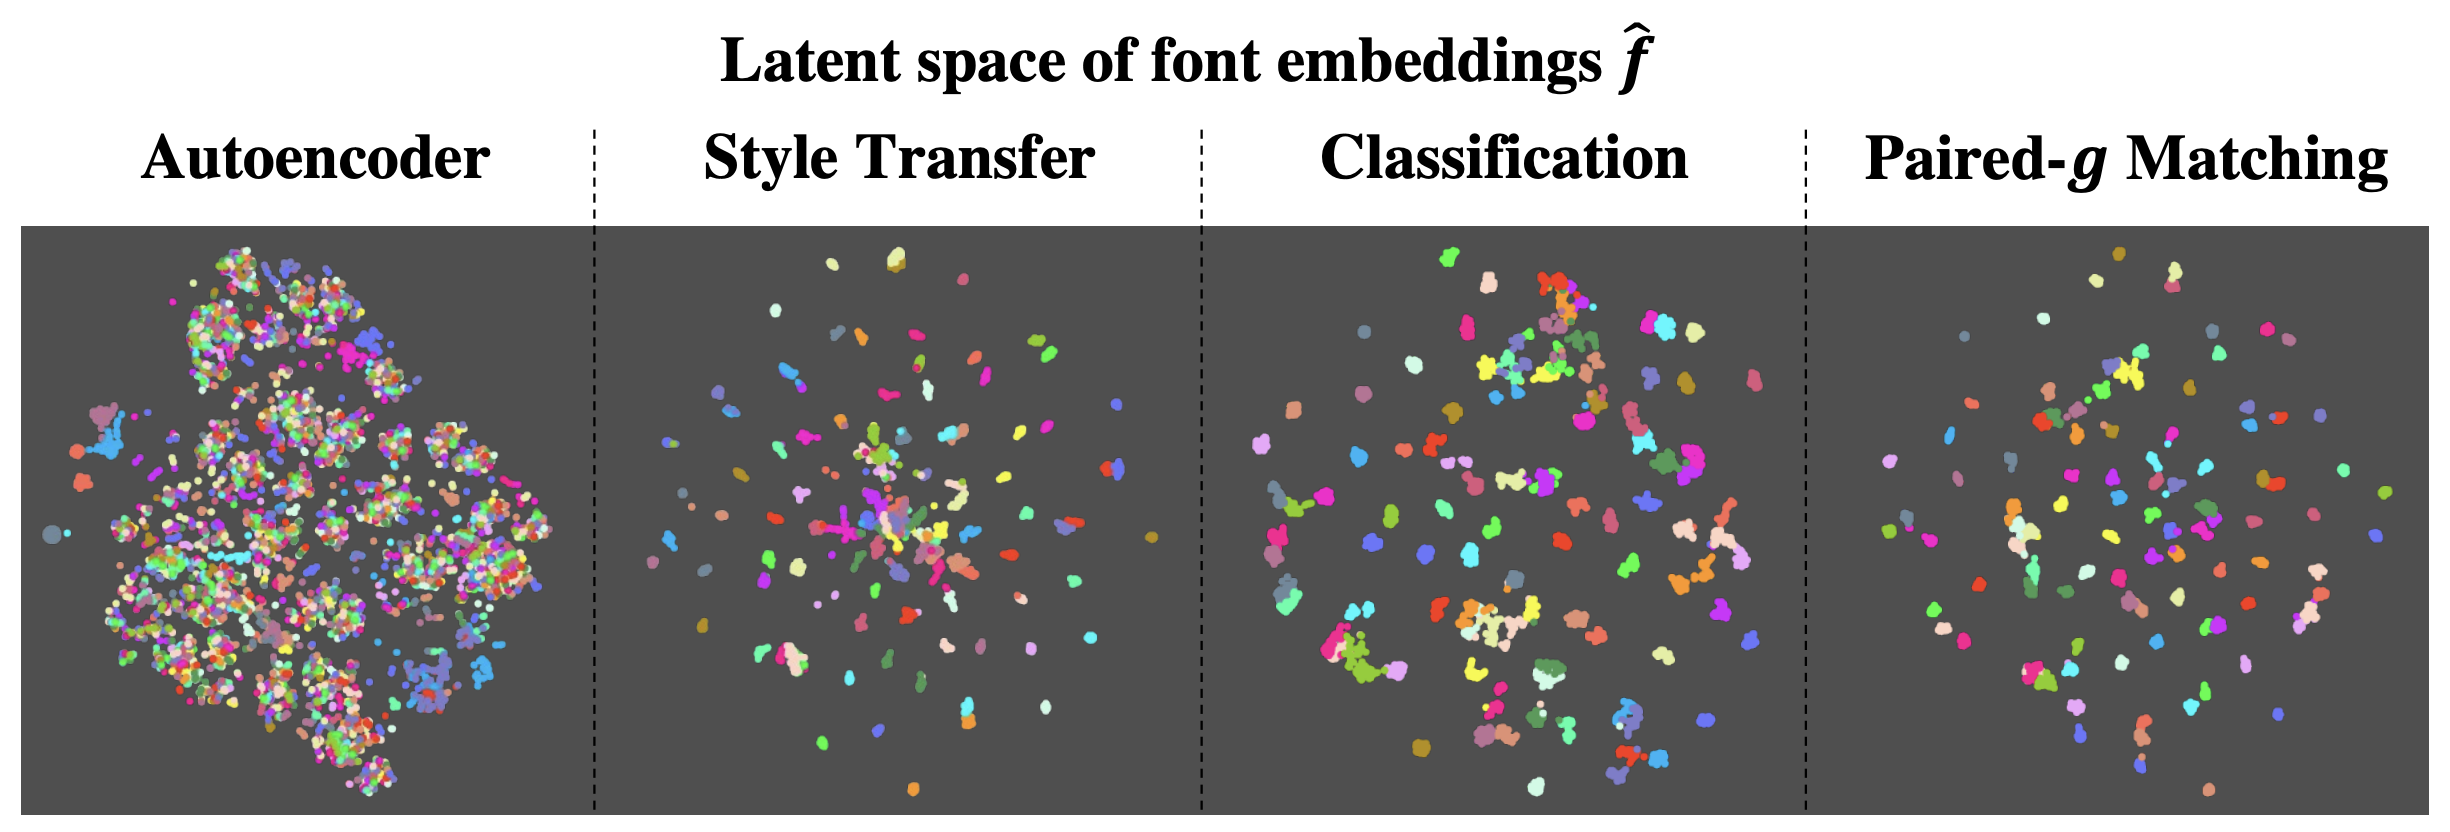
\includegraphics[width=1\textwidth]{images/cho-latent-space.png}
    \caption{Latent space of style embeddings across model techniques in Cho et al.\ \cite{cho2022}, with color representing the typeface of a given character style encoding}
    \label{fig:cho-latent-space}
\end{figure}

Relevant to our work is their evaluation of different model architectures for generating style encodings. As shown in the latent space maps in Figure \ref{fig:cho-latent-space}, they employ three different model architectures in addition to their paired-glyph matching: the basic autoencoder model, style transfer (generating another character in the same font given an input character), and classification (predicting which font is represented in a glyph). There is an overlap in some of their model choices and ours (namely, autoencoder and style transfer), and the figure they provide is useful in visualizing the typeface-clustering effectiveness of these various models.

\begin{figure}[]
    \centering
    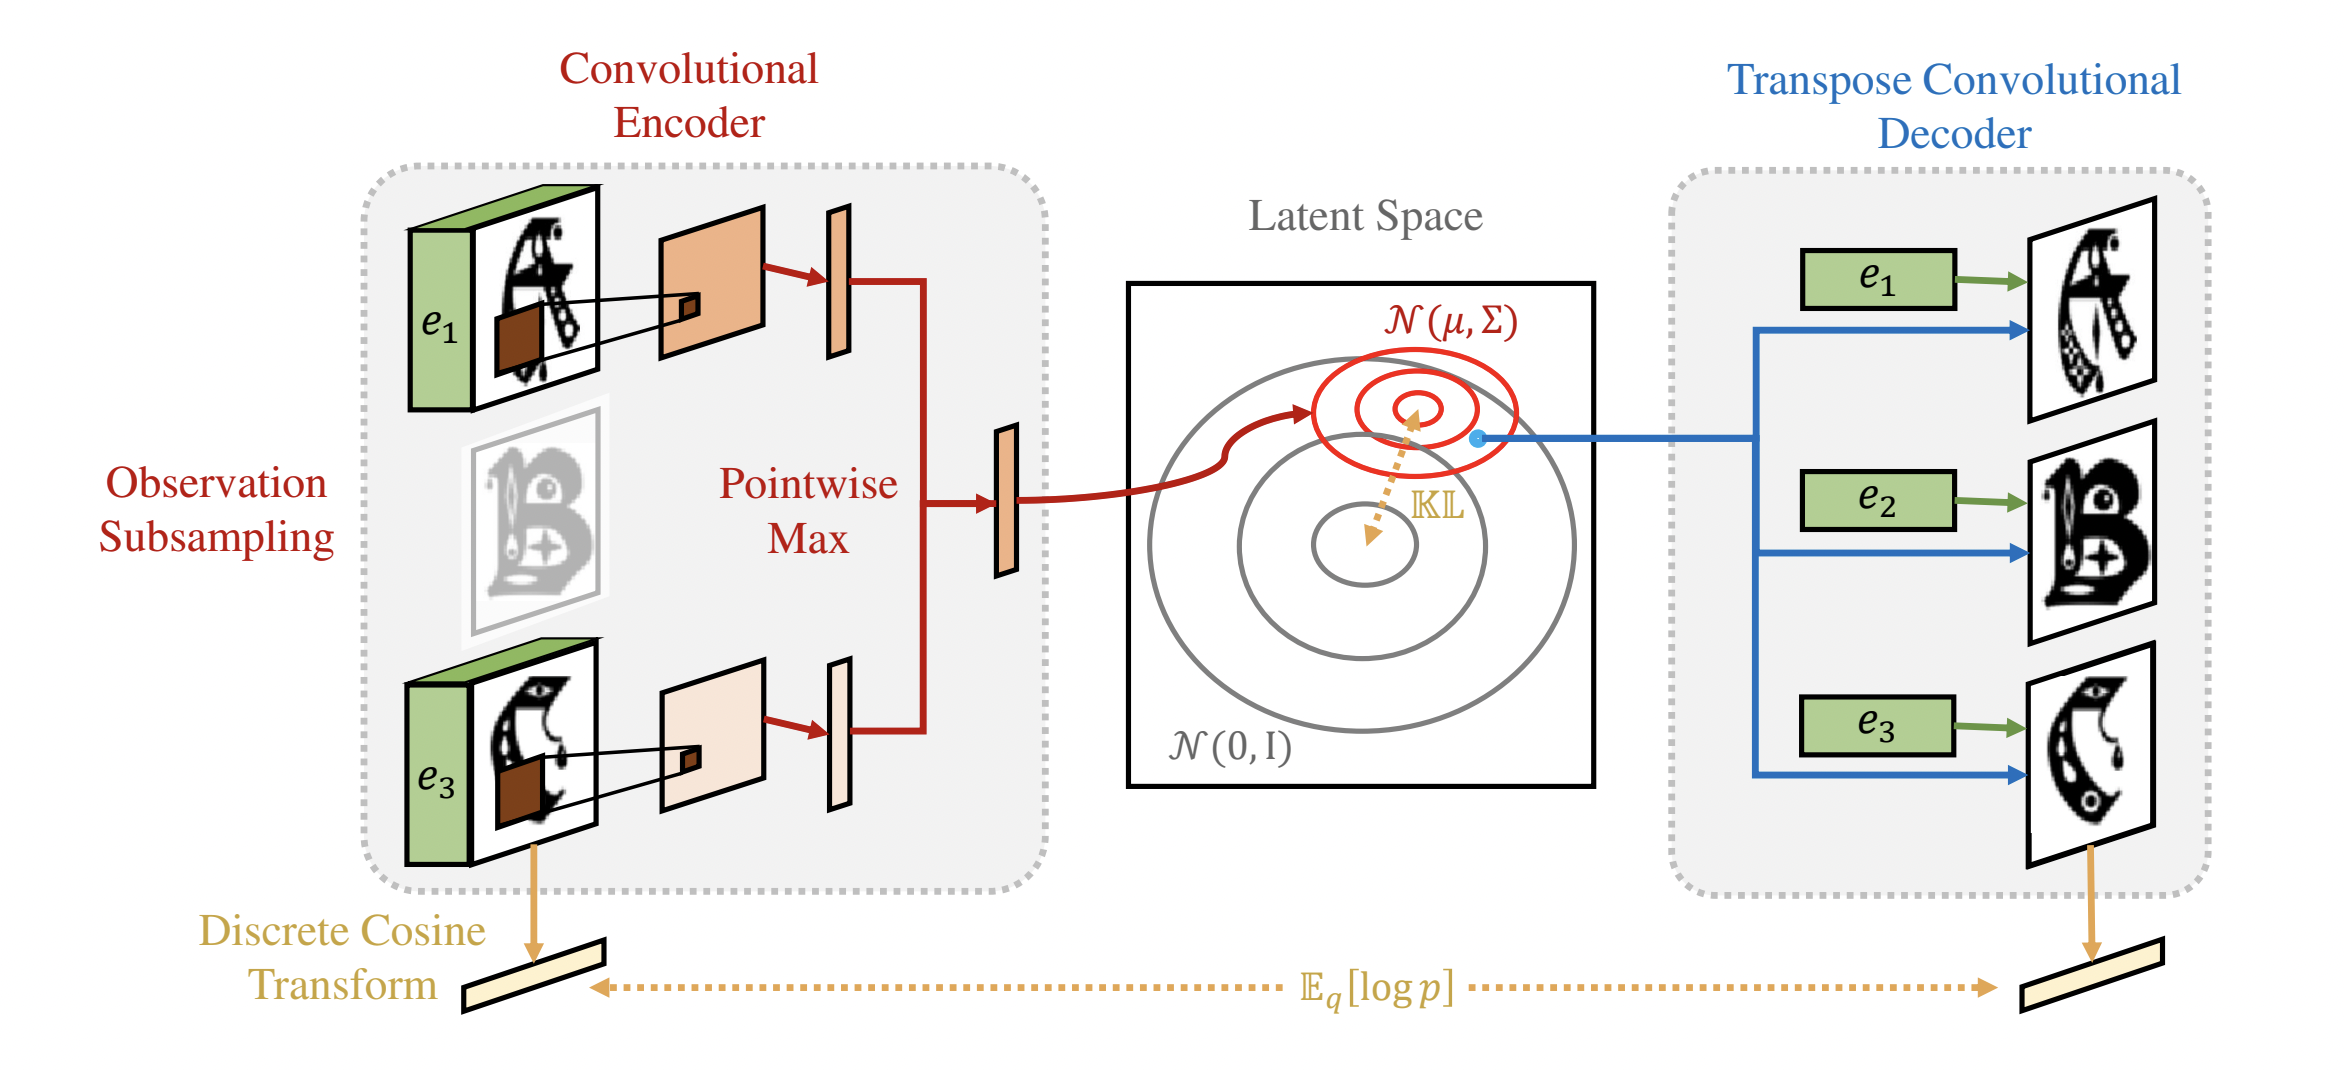
\includegraphics[width=1\textwidth]{images/srivatsan-model.png}
    \caption{Generative process of model from Srivatsan et al.\ \cite{srivatsan2020}}
    \label{fig:srivatsan-model}
\end{figure}

Srivatsan et al.\ \cite{srivatsan2020} introduce a training method based on latent probability space and a tensor factorization approach well-founded in past literature \cite{freeman1997,tenenbaum2000,vasilescu2002,tang2013}. Their model explicitly seeks to disentangle style and content—to encode the typeface style of a glyph as separate from the actual character it represents. The model architecture, shown in Figure \ref{fig:srivatsan-model}, convolutionally encodes a probabilistic encoding of a font given its complete character glyph set (with a chosen number missing) and corresponding character embeddings, and uses that latent probability vector along with a given character embedding to reconstruct the missing glyphs. Their model is particularly effective at reconstructing glyphs, when compared to peer models, and it also succeeds against a state-of-the-art peer model \cite{azadi2017} when evaluated by humans on Amazon Mechanical Turk. The model additionally yields high quality style encodings, with similar fonts having similar encodings in the model space. Figure \ref{fig:srivatsan-latent} shows a t-SNE projection \cite{vandermaaten2008} of their model latent space with ``A'' glyphs displayed at each centroid given k-means clustering ($k=10$). These centroids are representative of the typeface styles existing at the given area of the t-SNE plot. Lastly, Srivatsan et al.\ find that, qualitatively, their model seems to effectively recreate many important aspects of character style including shape, shadow, and texture.

\begin{figure}[]
    \centering
    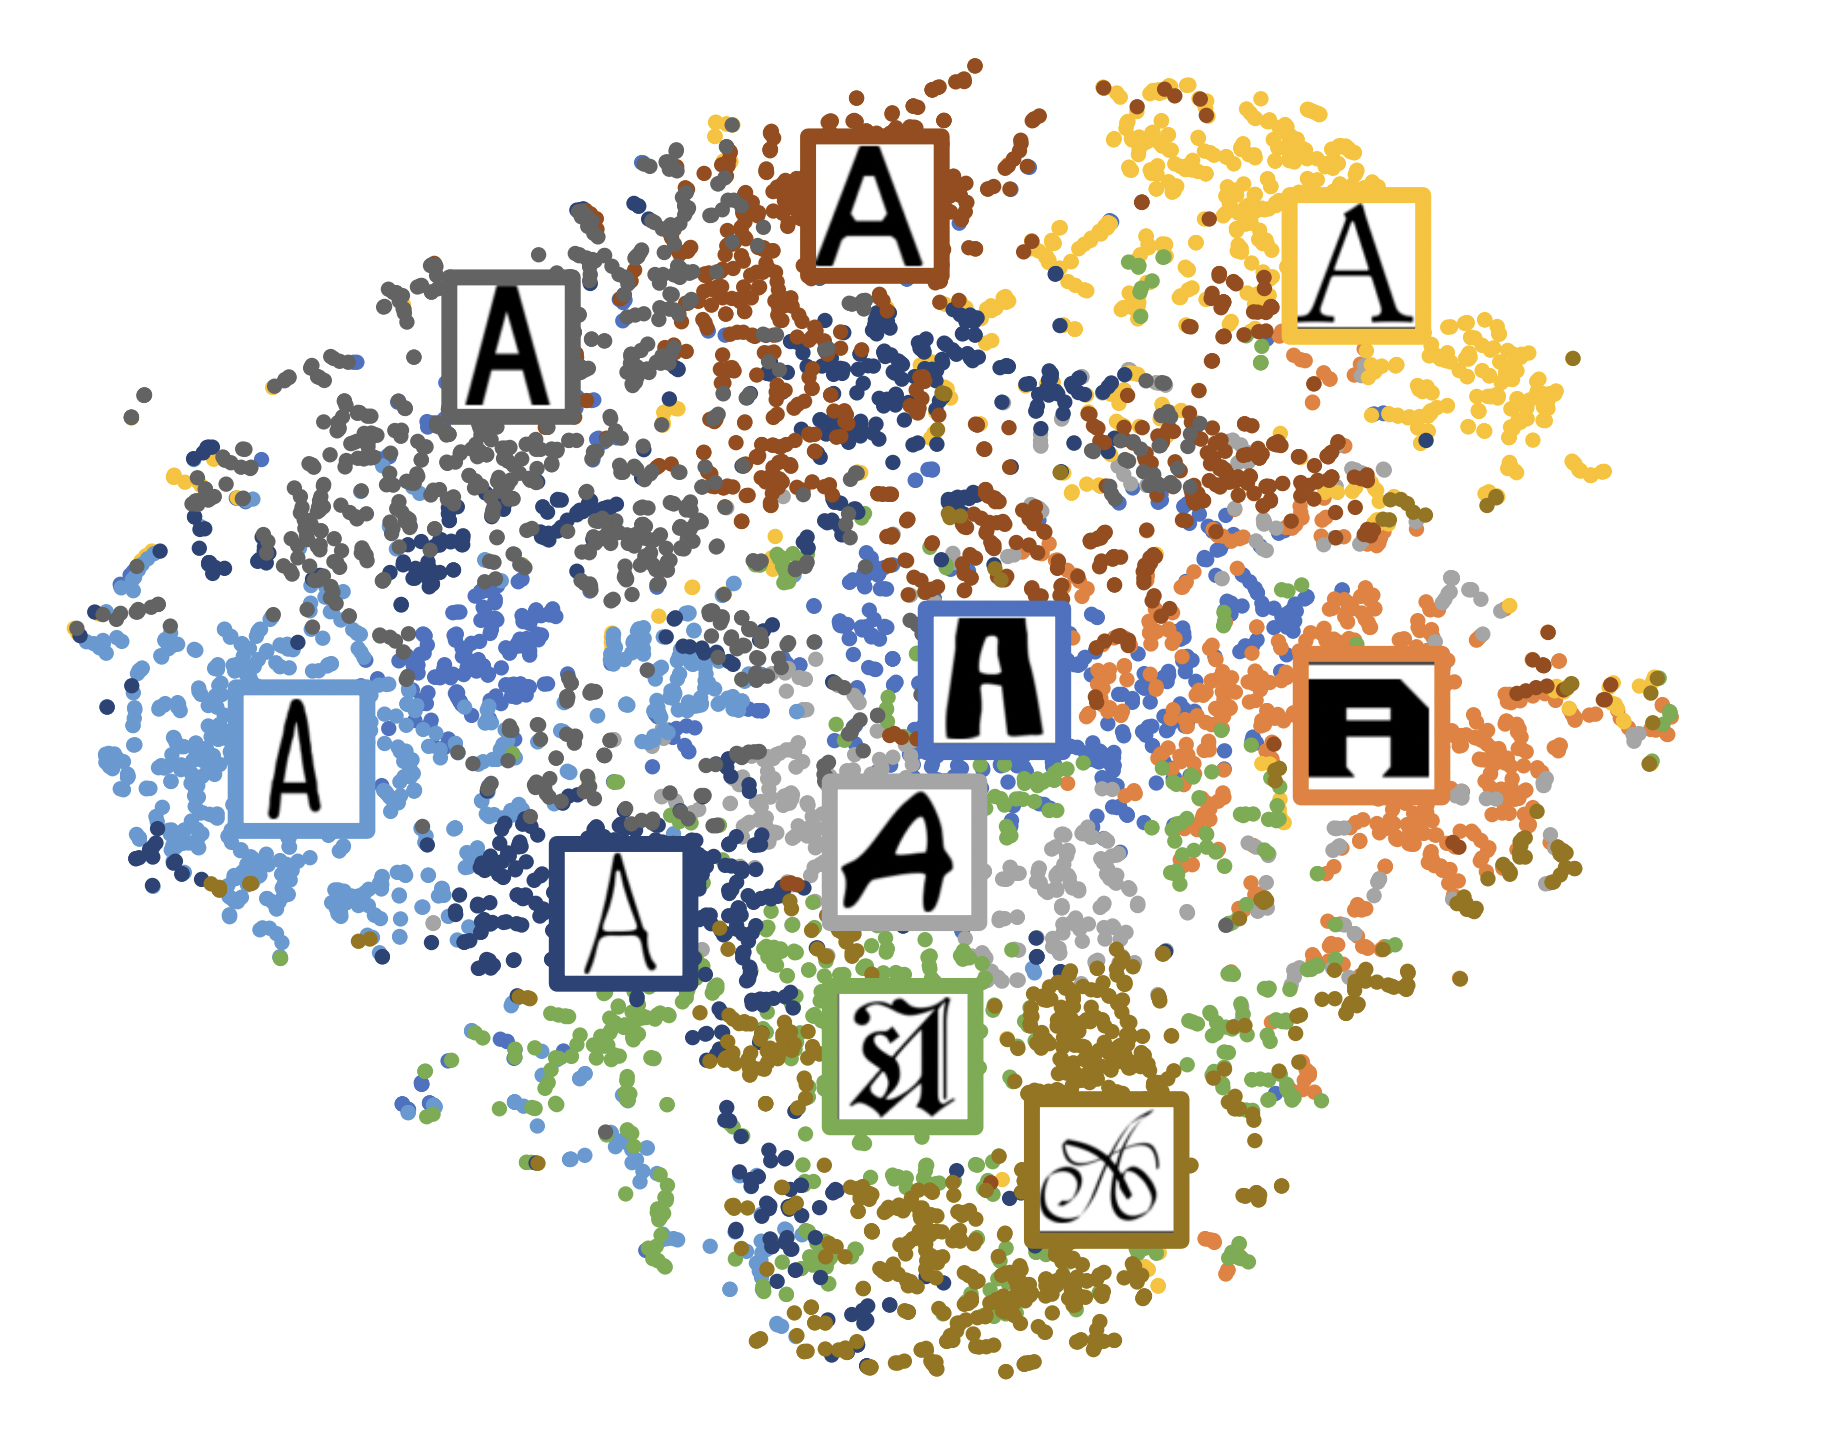
\includegraphics[width=.7\textwidth]{images/srivatsan-latent.png}
    \caption{t-SNE projection of latent font variables in Srivatsan et al.\ \cite{srivatsan2020} with centroids}
    \label{fig:srivatsan-latent}
\end{figure}

As previously stated, we chose to adapt the Srivatsan model in our research, porting it to a more recent version of Python (3.13) and PyTorch (2.5.1) and training the model on a larger dataset, comprised of the model's original training data, preinstalled Apple fonts, and the set of fonts available from the Google Fonts repository. We implement this model, along with two of our own models, and compare their respective style encodings in the following sections.
\chapter{Model and System Design}
\label{chap:methodology}

\section{Data Collection} \label{data-collection}

In order to train models to effectively encode the style of typefaces, it was necessary to create a dataset of characters from a wide variety of fonts. Given the stylistic diversity between fonts, it was important that the dataset be large and representative enough to encompass the variety of existing typeface styles---so that the model would work effectively not just for fonts in its training set, but for unseen fonts as well.

The first important consideration was the source of our data. The model proposed by Srivatsan et al. \cite{srivatsan2020} was trained on the large Capitals64 dataset constructed by Azadi et al. \cite{azadi2017}. We also chose to use this dataset, but opted to add some additional sources of fonts. Specifically, we included the entire library of fonts from the Google Fonts repository,\footnote{\url{https://github.com/google/fonts/}} which contains a wide range of free-to-use fonts, and we also included the default fonts which come preinstalled with macOS (which contains many of the well-known proprietary fonts not represented in Google Fonts or Capitals64). In the latter two cases, we only considered fonts which supported English-language text, choosing to ignore typefaces in other scripts (Chinese, Arabic, Bengali, e.g.) for the scope of this research. Ultimately, we included in our dataset 10,682 typefaces from the Capitals64 dataset, 3,577 from Google Fonts, and 132 fonts from the installation of macOS. We felt that this combined dataset ($n = 14,391$) would be both sufficiently large and representative of a wide variety of typeface styles, while still containing well-known proprietary fonts such as Times New Roman and Helvetica.

The fonts we sourced came as TrueType (.ttf) and OpenType (.otf) binary font files, both of which contain the raw data for individual typefaces or multiple typefaces in one family (Helvetica and Helvetica Light, e.g.). We used the open-source FontForge scripting package\footnote{\url{https://fontforge.org/en-US/}} to create an SVG vector image file for each character represented in each typeface, then rasterized the character vector files to $64 \times 64$ pixel images in PNG format. We additionally created $1664 \times 64$ images representing the 26 capital letters (A-Z) in each typeface to fit the Capital64 data format expected by the Srivatsan et al. model implementation. For font files which contained multiple styles in a given font family (e.g. Times, Times Italic, and Times Bold), we treated each style as a separate typeface, since their respective style representations should be meaningfully different.

\section{Models}

Over the course of our research, we employed several model training methods. This section details the various approaches and their respective model architectures. All models were trained using PyTorch 2.5.1 and Python 3.13 running on a Bizon G7000 G2 GPU server with 2x 32-Core 2.00 GHz Intel Xeon Gold 6338 CPUs and 4x NVIDIA RTX A6000 48 GB GPUs. Generally, we trained our models until the model loss plateaued, i.e. the font reconstruction task stopped improving.

\subsection{Basic Autoencoder} \label{basic-autoencoder-2}

For our first approach, we adapted the autoencoder model proposed in \cite{rumelhart1986}. As previously explained, an autoencoder is a neural network trained to compress and reconstruct input data. By doing so, it can learn to generate meaningful encodings of input data; in the case of our research, we hoped to capture typeface style in these model encodings. We implemented an autoencoder model trained on our large dataset of font character images, represented as pixel-intensity matrices. Our model uses a series of alternating linear layers and ReLU activation functions to compress the $64 \times 64$ pixel images (flattened to length-4096 vectors) down to length-6 vectors, approximately halving the size of the vector with each linear layer. The decoder, conversely, expands the representation back to its original size with a series of linear and non-linear layers, ultimately converting the vectors back into $64 \times 64$ pixel intensity matrices. To compute the loss of our model, we used mean squared error (MSE) between respective pixel values in the input and output matrices. After computing this loss, we translated the pixel intensity matrices back into their original image form, in order to visually evaluate the success of our reconstructions.

Some example input and output from our initial autoencoder model can be found in Figure \ref{fig:autoencoder-example}. Even early in the training, the model was able to accurately reconstruct most of the input characters, although it struggled more with more complicated typeface styles. However, we quickly identified an issue with this model: the autoencoder has no obvious incentive to distinguish form (the style of a character, defined by its font) from content (the actual letter which is represented). For example, an {\fontspec{Helvetica} A} in Helvetica looks substantively different than an {\fontspec{comicsans.ttf} A} in Comic Sans, but an {\fontspec{Helvetica} A} in Helvetica \textit{also} looks substantively different from a {\fontspec{Helvetica} B} in Helvetica, simply because they are different letters. Our basic autoencoder does not have sufficient information to decouple the stylistic similarity of Helvetica's {\fontspec{Helvetica} A} and {\fontspec{Helvetica} B} from the structural similarity of the the Comic Sans {\fontspec{comicsans.ttf} A} and the {\fontspec{Helvetica} A} in Helvetica. Under this model, the dimensions of the resulting style encoding likely conflate variance in style with variance in the characters themselves.

In order to create style encodings for style-based font selection, an effective model must be able to understand \emph{character} as separate from \emph{style.} Characters in the same font should all be understood to have one style, determined by the font itself, while two characters in different fonts should have different style encodings (which might be more or less similar depending on their respective styles).

% my own figure
\begin{figure}[H]
    \centering
    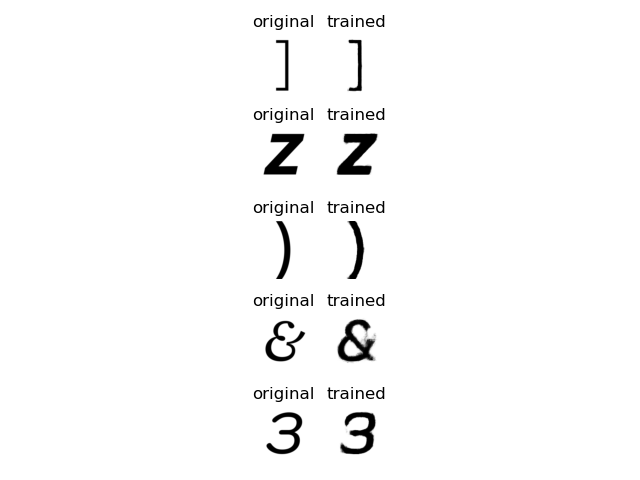
\includegraphics[width=\textwidth]{images/autoencoder-example.png}
    \caption{Our basic autoencoder model inputs/outputs mid-way through training}
    \label{fig:autoencoder-example}
\end{figure}

% my own figure
\begin{figure}[H]
    \centering
    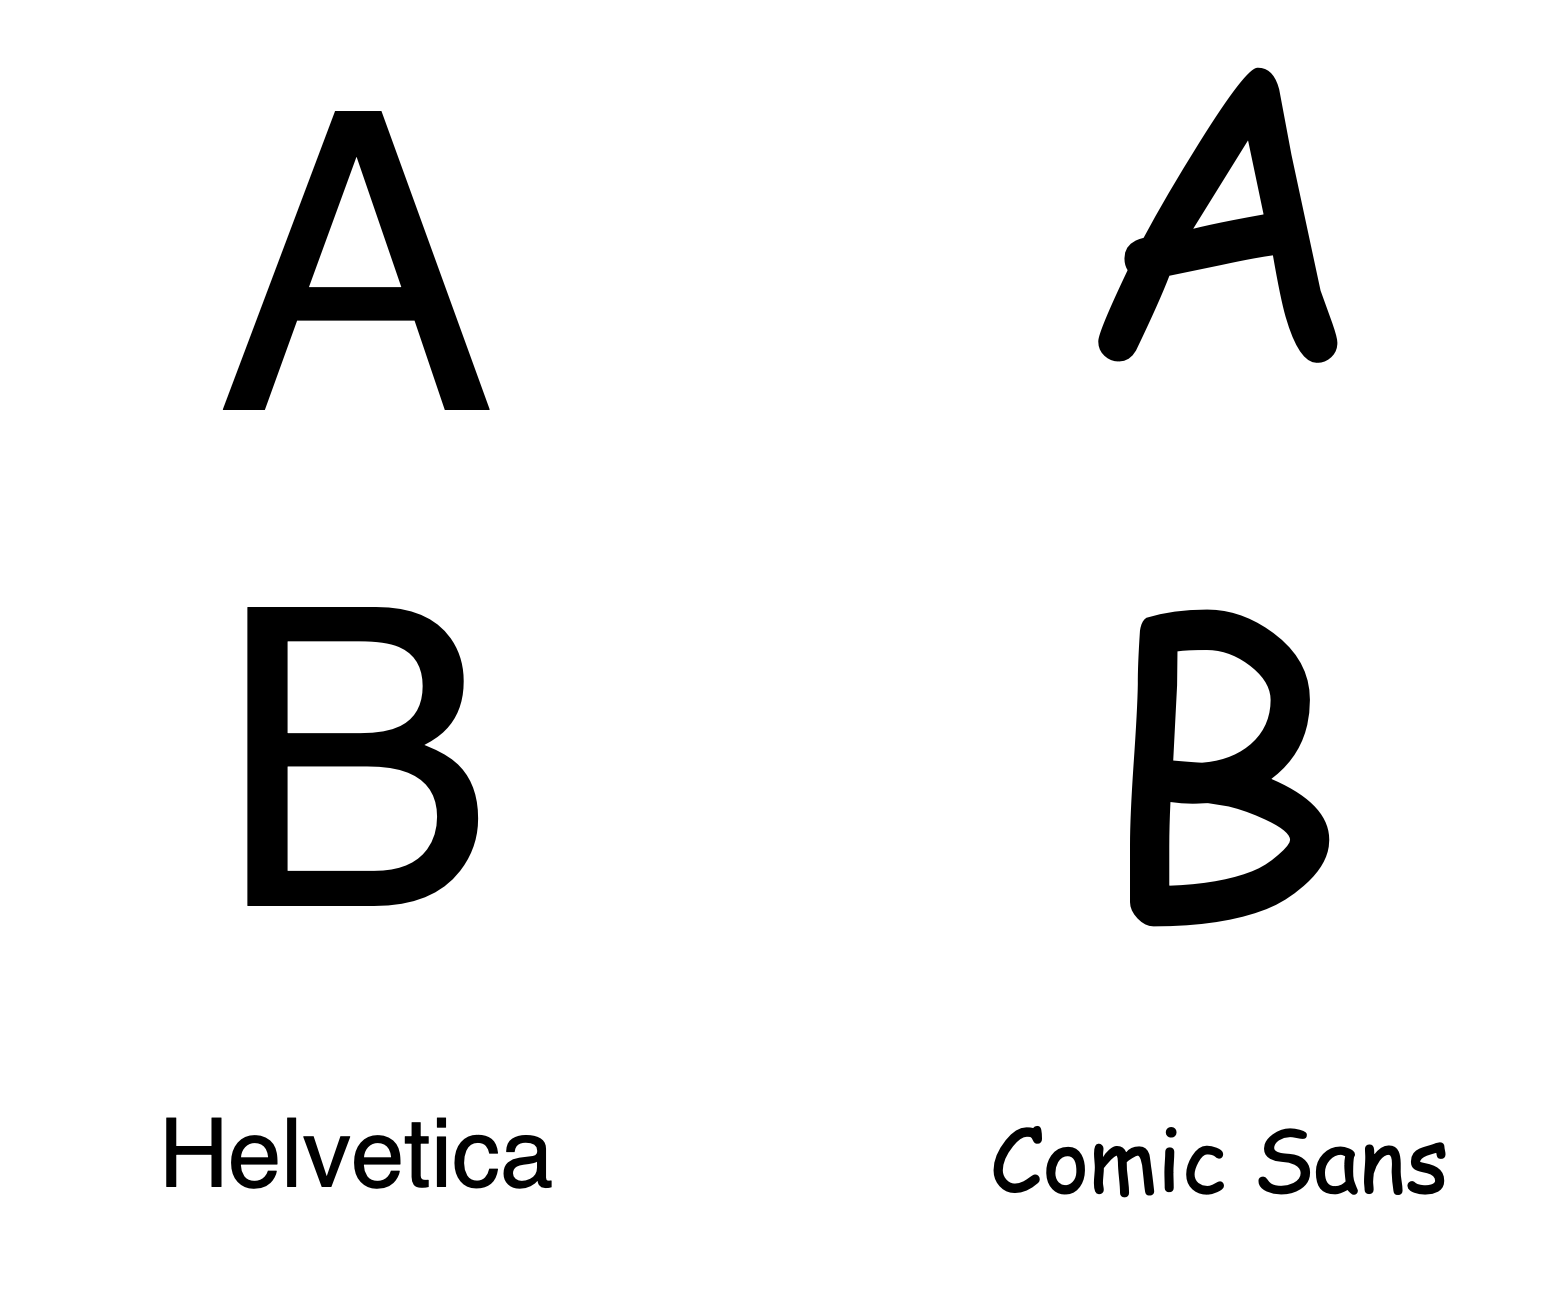
\includegraphics[width=0.55\textwidth]{images/ab-cs-helvetica.png}
    \caption{An {\fontspec{Helvetica} A} in Helvetica is more similar to an {\fontspec{comicsans.ttf} A} in Comic Sans than to a {\fontspec{Helvetica} B} in Helvetica}
    \label{fig:ab-cs-helvetica}
\end{figure}

\subsection{Style Transfer Autoencoder} \label{style-transfer}

To disentangle style from character, we trained a modified autoencoder on a different task: to recreate \textit{other} characters in a given font. For example, given an input image of a C character, we trained the model to output a Q character in that same font. In order to provide the necessary information for the model to succeed in this task, we included two additional vectors in the model input: one representing the character of the input image, and the other representing the target character. Figure \ref{fig:style-transfer-model} illustrates this schema. The model takes as input a characer image as input, along with the vector embedding parameter representing the character information, and additionally takes the target character embedding as a mid-way input to provide the decoding step with the requisite information to construct the target image. By minimizing the MSE between the generated character (say, a {\fontspec{Arial} Q} in Arial) and the ground truth image in our dataset, we hypothesized that our model would better isolate style in its encodings. The model has no need to represent character in the intermediate encoding, since both the encoder and decoder explicitly receive auxiliary character information. 

% my own figure
\begin{figure}[]
    \centering
    \includegraphics[width=\textwidth]{images/style-transfer-model.pdf}
    \caption{Our Style Transfer Autoencoder model, which attempts to recreate a different character in the typeface of an input character image}
    \label{fig:style-transfer-model}
\end{figure}

Importantly, the inclusion of auxiliary input vectors required that there be a fixed-size character set. We originally experimented with limiting our training data to only include fonts which contained all uppercase (A--Z) and lowercase (a--z) English characters; however, in order to incorporate the Capitals64 dataset---which only includes capital letters---we decided to limit our training only to fonts including the English uppercase letters. Fonts which did not contain the 26 uppercase letters A--Z were excluded from training.

For the style transfer model, we had to modify the data loading process. Rather than dealing with every individual character in a font, we needed to handle every \textit{pair} of characters in a font. Since we were considering 26 characters per font, our model trained on ${}_{26}C_2 =$ 325 character pairs per typeface. Additionally, since we were considering the input/output characters as data inside our model, unlike the basic autoencoder approach, we also created embeddings for each of the characters within our model architecture. The input embedding was concatenated with the flattened input image before it was fed to the encoder, and the output character embedding was concatenated with the intermediate vector representation between the encoder and decoder. Finally, we computed the MSE loss not against the input image but against the ground truth goal image representing the target character in the selected font.

Figure \ref{fig:styletransfer-example} shows our style transfer model part-way through training. The model receives the input {\fontspec{kumar-one.ttf} B} glyph and the input/output character embeddings (not shown), and it attempts to reconstruct the {\fontspec{kumar-one.ttf} h} glyph in the same typeface. By giving the model explicit vector representations of the input/output characters, we hypothesized that the model would more effectively isolate the style of the glyphs as separate from their content, giving us better internal representations to leverage for style-based typeface selection.

% my own figure
\begin{figure}[h]
    \centering
    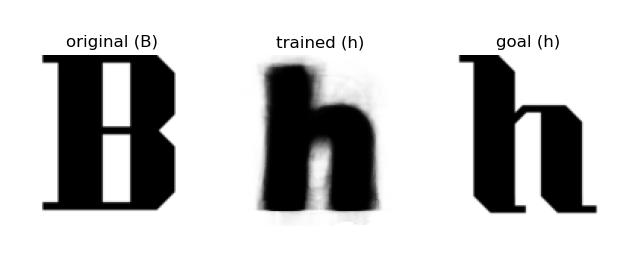
\includegraphics[width=\textwidth]{images/styletransfer-example.png}
    \caption{Example instance of our style transfer model part-way through training}
    \label{fig:styletransfer-example}
\end{figure}

\subsection{Srivatsan Model}

Our final model, which we adapted from Srivatsan et al.\ \cite{srivatsan2020}, mirrors our previous approaches in many ways, but it introduces several techniques hypothesized to improve the stylistic encoding ability of the model on our dataset. Most notably, the Srivatsan model incorporates variational inference and convolution. It may be necessary to define these terms: a variational encoder, rather than explicitly encoding an intermediate vector representation between the encoder and decoder steps, produces intermediate parameters $\mu$ and $\sigma$ of a multi-dimensional Gaussian distribution, from which a vector representation is randomly sampled and then decoded. Proposed by Kingma et al.\ \cite{kingma2019}, variational autoencoders (VAEs) are often used for generative tasks in deep learning, as they represent a large probabilistic space of outcomes. However, even in non-generative tasks such as ours, the variational model can generate useful, often more stable model encoding spaces.

Convolution, and convolutional layers---a technique which is separate from variational modeling but can be used in tandem with that technique, as in the case of the Srivatsan model---involves a moving filter called a kernel which reduces spatial dimension. In the case of typeface style encoding, this can be used to dissociate style elements from their particular location in training images. For example, the serif elements of a character in a serif typeface (i.e. the tail at the ends of characters like T and S) can appear at many different locations in a training image depending on the particular character and typeface; using convolutional layers allows the model to recognize these elements regardless of their specific location in an image. Therefore, a model can better identify serif elements across many different characters, locations in those characters, and serif typefaces.

% my own figure
\begin{figure}[h]
    \centering
    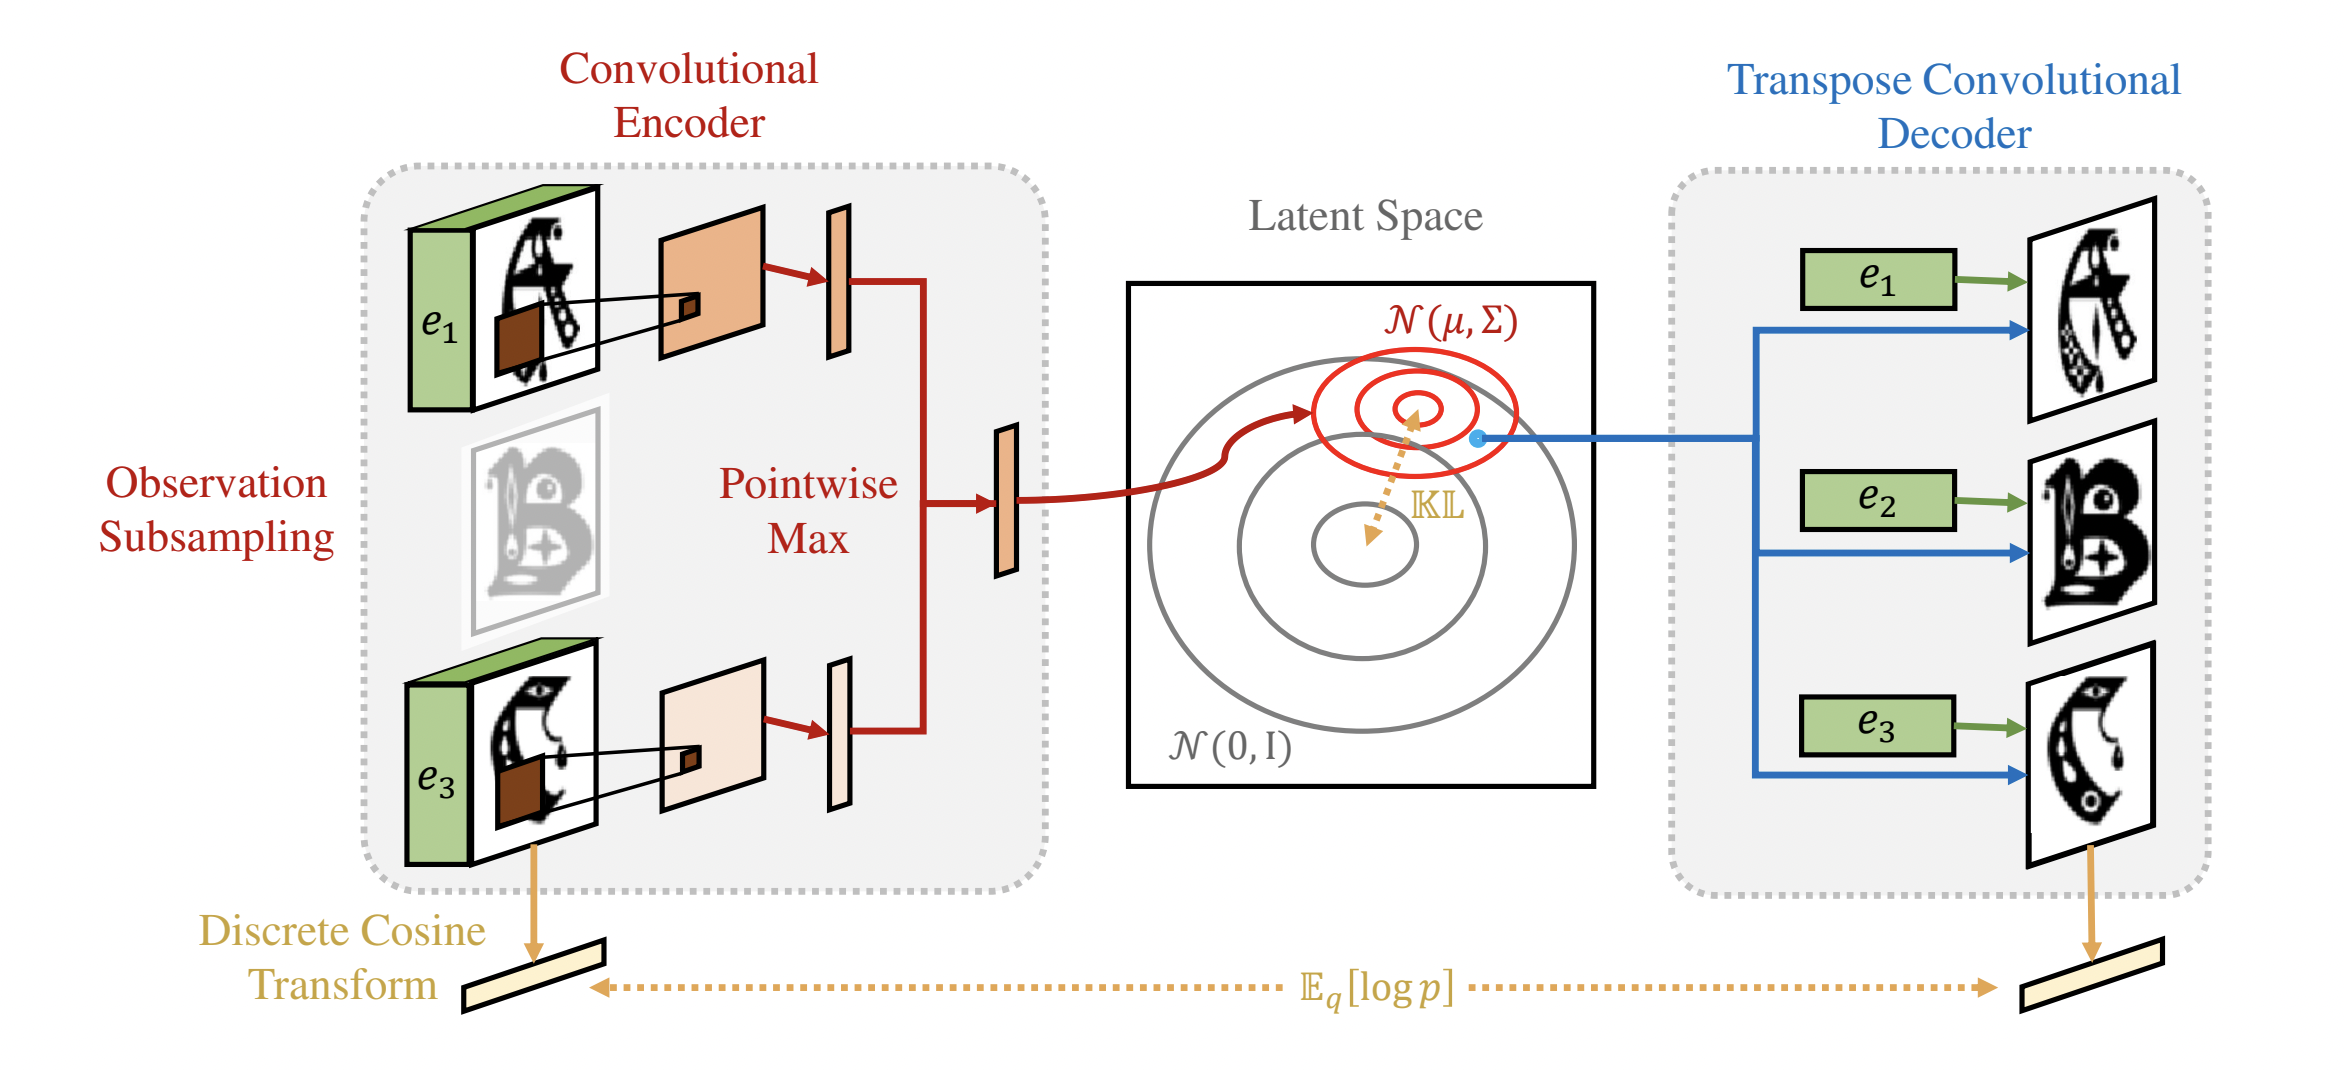
\includegraphics[width=\textwidth]{images/srivatsan-model.png}
    \caption{Diagram of Srivatsan et al.\ model architecture}
    \label{fig:srivatsan-model-2}
\end{figure}

Lastly, the Srivatsan model approaches style encoding using a slightly different task: it includes a full set of characters as input data for character reconstruction, and it approaches the character reconstruction task across an entire typeface at once---rather than reconstructing each character or character pair individually. Similar to our Style Transfer model detailed in \ref{style-transfer}, the Srivatsan model aims at recreating different characters across a typeface and involves vector character embeddings for those input/output characters; however, the model takes the full set of uppercase characters A--Z and randomly masks a set number of characters for reconstruction, rather than dealing with characters individually. The model reconstructs the missing characters based on the given (non-hidden) characters in the font, as well as the character embedding information for the hidden characters. The encoder creates a Gaussian encoding from the input, and the decoder uses that encoding along with the respective respective character embedding for the masked glyphs to reconstruct the full character set for a given typeface. The model also applies a 2-Dimensional Discrete Cosine Transform (2-D DCT-II) \cite{ahmed1974} to the generated images before computing the loss, with the goal of generating sharper images. DCT-II is simply a rotation in vector space, meaning the resulting probability measurements and vector distances are preserved. A diagram of the Srivatsan model architecture can be found in Figure \ref{fig:srivatsan-model-2}.
 
The Srivatsan model does an adequate job at glyph reconstruction---one of the focuses of the paper---but also generates promising style encodings. Figure \ref{fig:srivatsan-tsne} shows a t-SNE \cite{vandermaaten2008} plot of the latent style encodings generated by the Srivatsan model, colored by both weight and Google Font style category. As the figure shows, it is quite effective at clustering fonts with similar weight (bolder or lighter) and more ambiguous stylistic aspects provided as metadata with Google Fonts.

% my own figure
\begin{figure}[h]
    \centering
    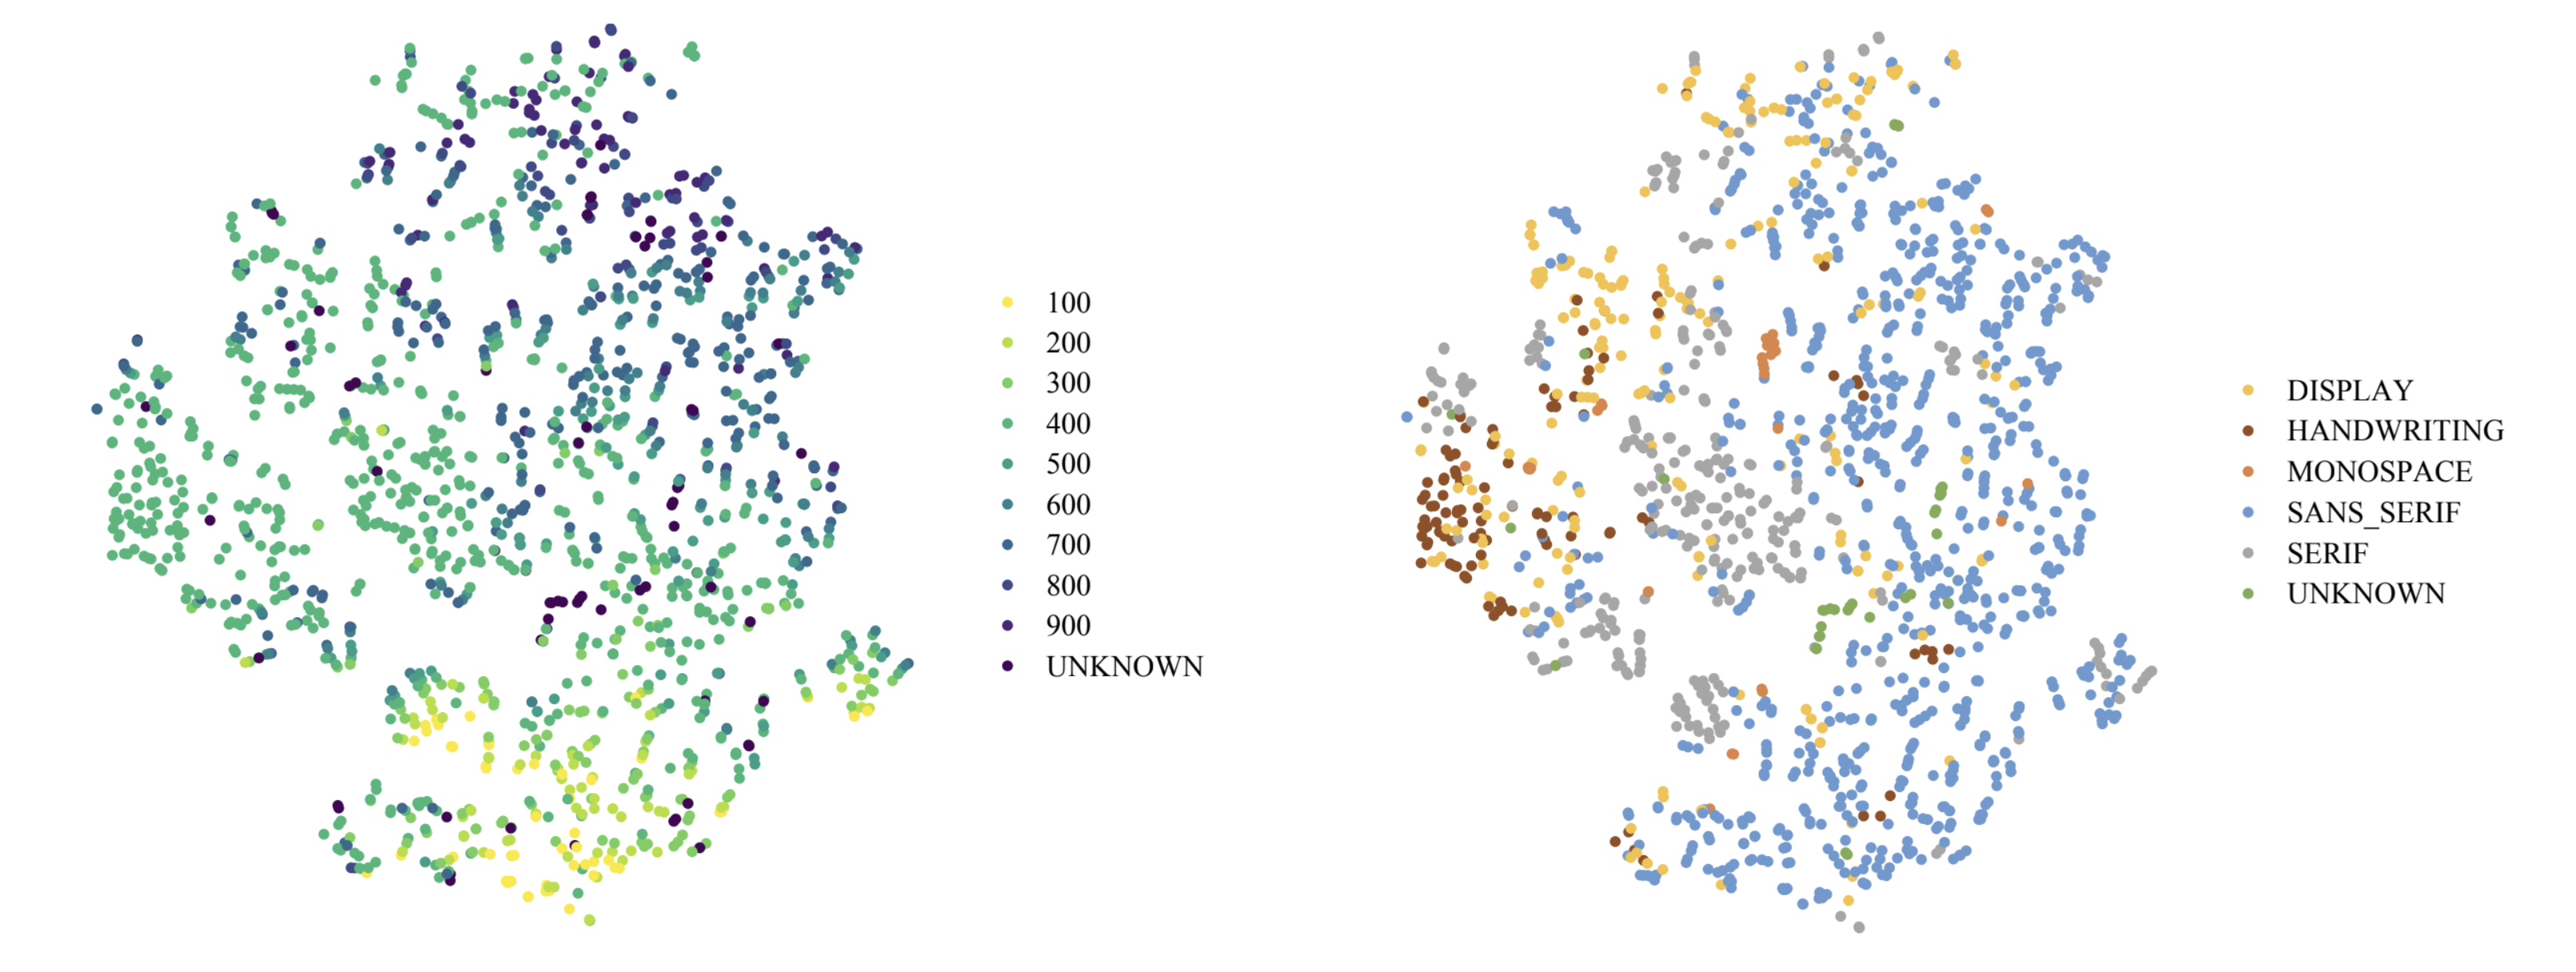
\includegraphics[width=\textwidth]{images/srivatsan-tsne.png}
    \caption{t-SNE plot of style encodings from Srivatsan et al.\ \cite{srivatsan2020} colored by weight (left) and Google Fonts style category (right)}
    \label{fig:srivatsan-tsne}
\end{figure}

We ported the original code from Srivatsan et al.\ \cite{srivatsan2020} from Python 2.7 and PyTorch 1.1.0 to Python 3.13 and PyTorch 2.5.1 and trained it on our extended dataset, with 10 hidden characters per font, for 184 epochs. After training, we ran the model on a modified version of our Google Fonts dataset in order to generate useful style encodings which we could compare against our other models and use in our webapp font selector tool. As with our other models, we trained the modified Srivatsan model until the MSE loss plateaued and the model seemed (by visual inspection) to adequately reconstruct the missing characters for most input character sets.

Figure \ref{fig:srivatsan-reconstructions} shows 44 reconstructed character sets from the Srivatsan model, with 10 out of 26 characters reconstructed by the model. The model seems better at reconstructing some fonts than others---specifically, it seems to have performed better on typefaces with more common styles, such as basic serif or sans-serif fonts. Stranger, more uncommon font styles were not reconstructed as accurately (for example, the third font from left in Figure \ref{fig:srivatsan-reconstructions}). However, character reconstruction is not out primary objective. Our main goal is to encode typeface style using the intermediate representation of the model, which does not correspond exactly with the model's character reconstruction ability. Nevertheless, the highly accurate reconstruction performance we see for many of the typefaces, along with a somewhat-decent reconstruction of the more difficult fonts, suggests a fairly strong representation of typeface style within the model. Further evaluations in Chapter \ref{chap:evaluation} will quantitatively analyze the style-encoding capabilities of our three models.

% my own figure
\begin{figure}[h]
    \centering
    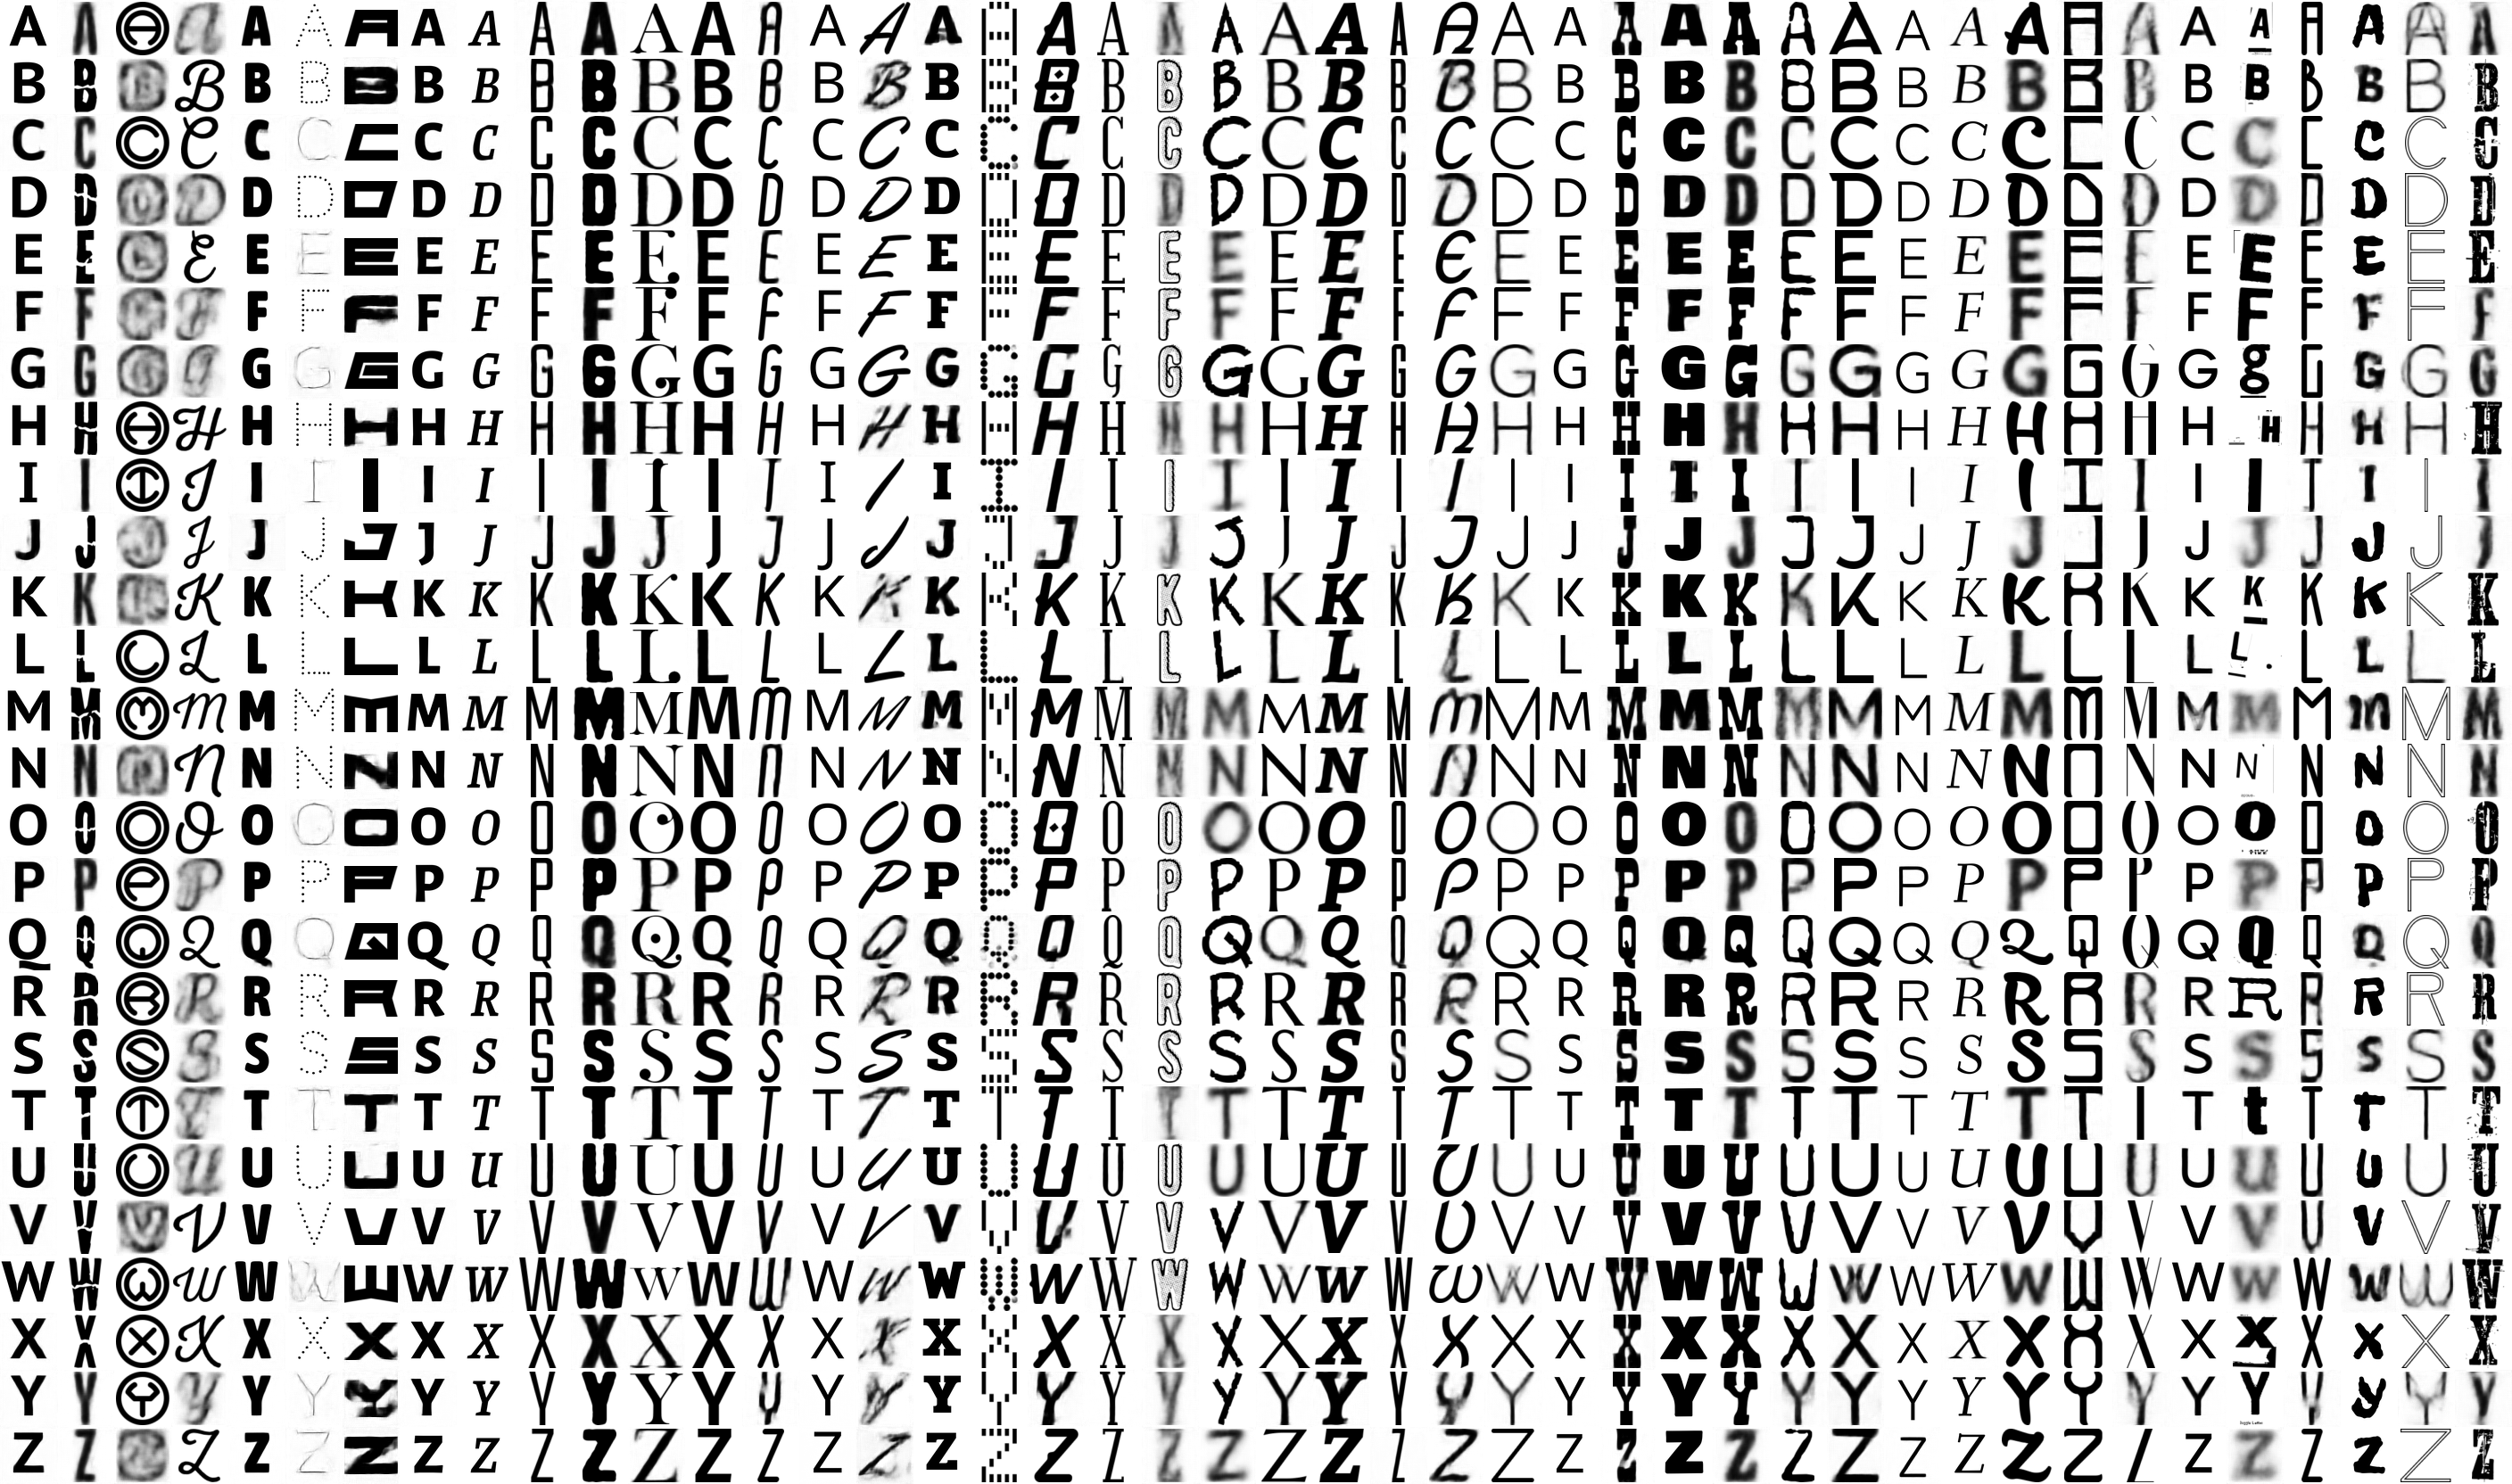
\includegraphics[width=\textwidth]{images/srivatsan-reconstructions.png}
    \caption{Reconstructed character sets from the adapted Srivatsan model}
    \label{fig:srivatsan-reconstructions}
\end{figure}

\subsection{Extracting Style Encodings}

In order to build useful typeface selection tools based on these models, it was necessary in all three cases to extract the model's internal style encoding vector for each typeface. This task was relatively trivial for the first two models: we simply passed each of the typeface character sets through the encoder portion of our model and performed an elementwise average across the resulting vector representation for each character, which we believed would generate a roughly-representative style encoding for the entire typeface. For the Srivatsan model, we similarly ran our model on each of the typeface character sets; however, since the Srivatsan model applies a variational approach, it was additionally necessary to perform a random sample from the Gaussian distribution defined by each typeface character set to obtain a style encoding. Because the architecture of the Srivatsan model does not train on individual character sets or pairs, but entire typeface character sets together, it was not necessary to take an average of multiple character style encodings; the model, by design, trains one generalized latent style encoding for each typeface.

\section{System Design}

In this section, we detail the process and design of turning our style encodings—generated by the models in the previous section—into a user tool for typeface selection. We consider questions of encoding dimensionality, end-to-end system design, and user experience in order to create a novel, useful typeface selector tool.

\subsection{Style Encoding Dimensionality}

One initial question which emerges when training autoencoder-like models---especially with the goal of extracting intermediate encoding vectors---is: what should be the dimensionality of those encodings? In our case especially, there is a tradeoff between encoding more information (higher dimensional vectors should be able to represent greater stylistic detail, to a certain point) and usability (lower dimensional vectors represent fewer choices for users, presumably yielding easier-to-use tools). One could, for example, train a model to generate 2-dimensional style encodings; this could yield a very straightforward interface, such as a scatterplot of typefaces or two sliders corresponding to the two style axes, but two dimensions may not have the capacity to represent the many diverse aspects of typeface style. Alternatively, one could choose a high dimensional style encoding—say, a 100-dimensional vector—which would have a greater capacity to encode font style; however, presenting a user with a decision for each of those dimensions would be unwieldly and overwhelming.

We tested several embedding dimensions, but ultimately chose to encode typeface style using 6-dimensional vectors. This provides substantial capacity to represent typeface style, but also reasonably limits user choice. In the following section, we will describe how these six dimensions translate to a novel font selection tool; additionally, we compress these 6-dimensional style encodings into 2-dimensional space using t-SNE reduction to create an auxilliary scatterplot tool which provides users with an additional graphical representation of the data.

\subsection{User Experience}

We experimented with several iterations of a tool for intuitively exploring a space of high-dimensional style encodings. As mentioned previously, the question of dimensionality is a significant one when generating style encodings for user interaction; another important consideration is \textit{how} users should interact with these high-dimensional vector spaces. Should users have full control over each dimension, or should they be guided in their decisions? How should high-dimensional space—which cannot be easily visualized or conceptualized by users—be represented? What additional features (a back button, the ability to save a typeface for later reconsideration, a search bar) would help a user navigate this high-dimensional stylistic vector space? Moreover, what is the goal of our user (finding a specific font, finding similar fonts to a given font, or open exploration)? How much time is the user willing to spend searching for a font? What does the user want to do with this font (or fonts) once identified, and how can we assist the user to accomplish that?

\subsection{Lessons from Early User Tool Implementation}

Early in the development process, we implemented a user tool which included a numerical slider for each dimension of the model space and allowed users to generate new characters based on the model---namely, by inputting the user-determined vector into the model decoder and displaying the output generated character. Our goal was to visualize the dimensions of the model space, to see what sort of information about the characters were being encoded by the model. There were a few issues with our approach: first of all, the interface was inherently a generative task---users would generate new characters/typefaces rather than selecting a preexisting typeface in a dataset---which is a sort of task we later gave up (mostly because the resulting generated typefaces just don't look very good); secondly, this earlier interface was built atop our Basic Autoencoder model, meaning the different dimensions dictated by the sliders would change both style and character at once. Our most important takeaway, however, was that the tool afforded users too much control and not enough guidance while exploring fonts. Even with a relatively low-dimensional space like ours, giving users direct control over several continuous sliders did not make for a very good user tool. Our current interface, while still providing many different methods and dimensions of user control, is a bit more limited and guided with its options, hopefully making for a more useable tool.

\section{Current Interface}

The current iteration of our typeface selector tool involves two connected user tools which allow users to explore our 6-dimensional vector style space in complementary ways. The first tool is an interactive scatter plot, displaying a t-SNE reduction of our 6-dimensional style space. t-SNE \cite{vandermaaten2008} is a dimensionality reduction technique, which allows typeface encodings near each other in the original 6-dimensional space to generally remain close to each other in the reduced 2-dimensional space. The scatterplot is an intuitive and familiar representation of spatial data to most users, making it a useful tool for navigating this style-embedding space. Users can explore the scatterplot space and visualize the fonts represented at each point; if a user identifies a font with desireable qualities, they should be able to find similar fonts by exploring the points nearby.

% my own figure
\begin{figure}[h]
    \centering
    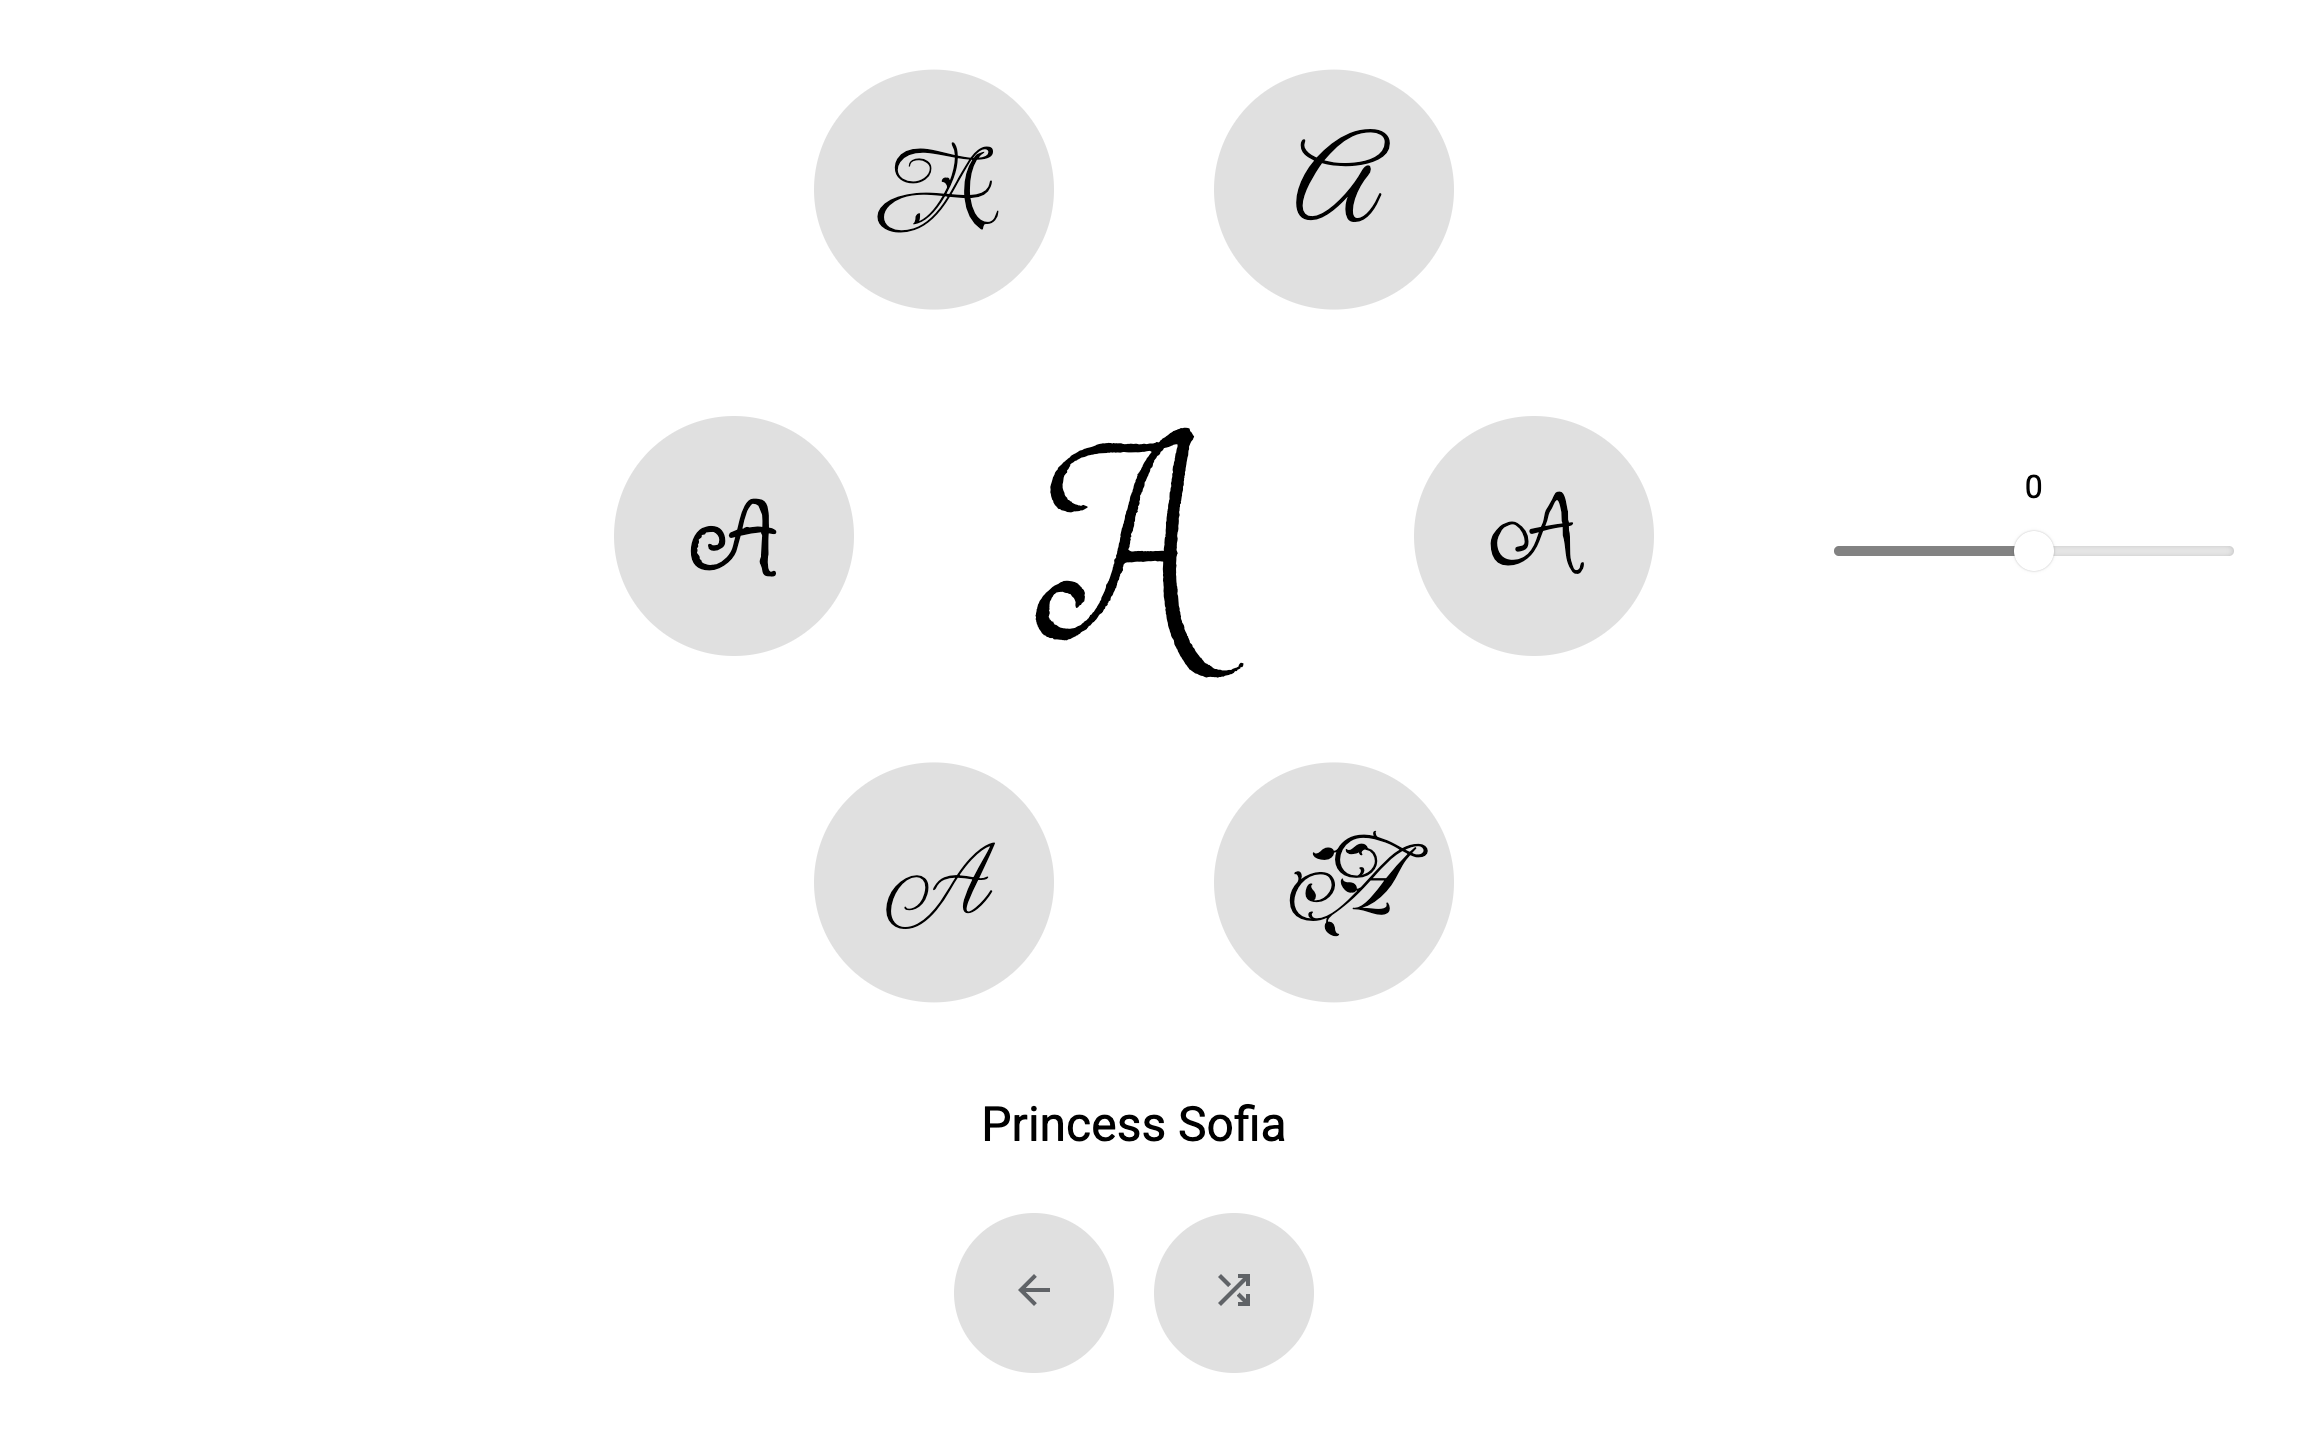
\includegraphics[width=\textwidth]{images/selector-tool.png}
    \caption{Our novel 6-dimensional typeface selector tool, displaying several similar calligraphic fonts nearby the Princess Sofia typeface}
    \label{fig:selector-tool}
\end{figure}

In order to provide another way for users to interact with this style space—one which preserves the dimensionality of our style encodings and therefore allows users full range over the model space—we include another typeface selector tool based on the 6-dimensional structure of our encoding data. This tool, shown in Figure \ref{fig:selector-tool}, displays a center font glyph (A is the default character, but this can be changed by the user) of a selected typeface in the model space, and shows six alternative typefaces of that font in a circle surrounding it. The slider, on the right hand side, represents magnitude; when the magnitude is zero, the six surrounding fonts represent the nearest neighbors to the center font (determined by Euclidean distance); when the magnitude is nonzero, the tool will search—along all six dimensions of the model space—according to the distance defined by the slider magnitude, and display the closest font in each of those dimensions. Therefore, as the slider grows further from zero, the six fonts displayed will have increasingly different style from the center font. At any point, a user can select one of the six surrounding fonts and move to that point in the model space, at which point the slider resets to zero (nearest neighbor), and the user may continue the process again in order to find a more optimal font. The tool also includes a shuffle button, enabling the user to randomly select a new font, and a back button which allows the user to return to previously seen fonts. By providing easy-to-use buttons and dynamically displaying fonts, this tool enables users to navigate a high-dimensional model space which is difficult to conceptualize intuitively.

% my own figure
\begin{figure}[h]
    \centering
    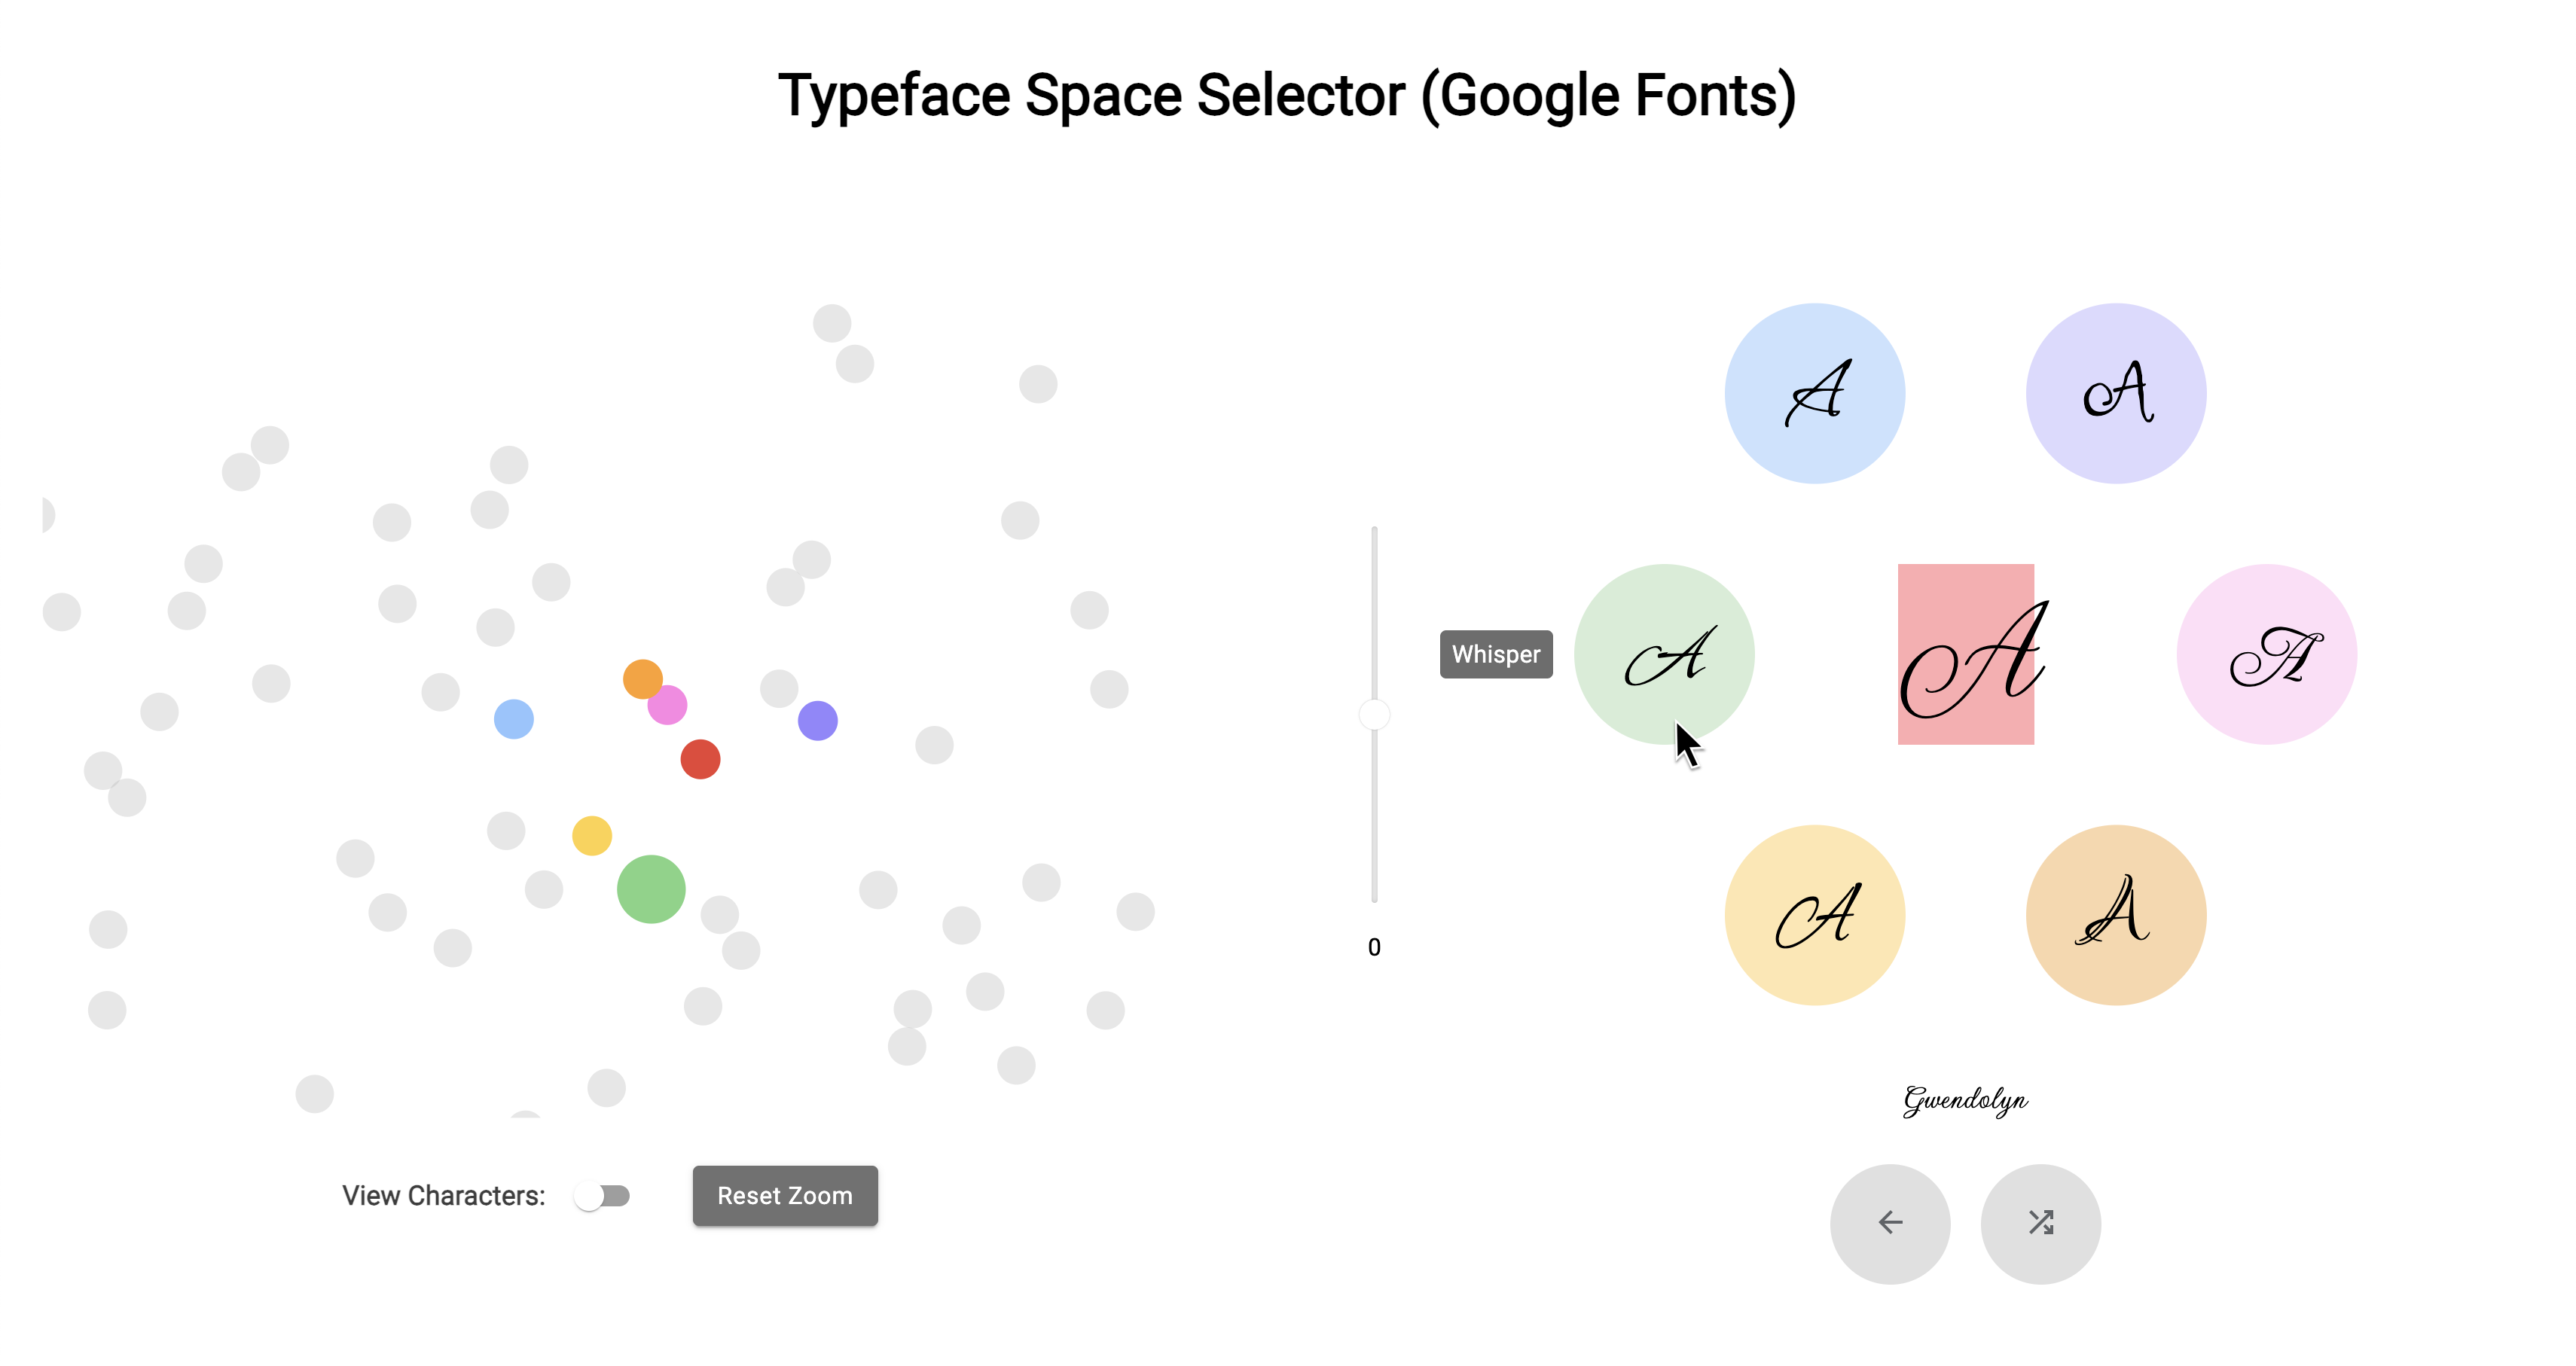
\includegraphics[width=\textwidth]{images/both-selectors.png}
    \caption{Both of our typeface selector tools side-by-side, with additional features to ease use of both tools in tandem}
    \label{fig:both-selectors}
\end{figure}

Our final product combines both the scatterplot and six-point tool, with several additional features to make the tools work together effectively (see Figure \ref{fig:both-selectors}). Namely, we use distinct colors to display the location of each of the typefaces from the 6-point selector tool within the scatterplot visualization. Additionally, when the cursor hovers over one of the typefaces in the 6-point tool, that point grows bigger in the scatterplot tool, making it even easier and clearer to locate a typeface within the t-SNE scatterplot space. Users can click on points in both the scatterplot and the 6-point selector, and the entire tool will dynamically update to the new typeface location. Finally, there is a toggle under the scatterplot to display characters instead of circular points (maintaining colors) which makes for an easier visualization of the entire space, and users can also zoom and pan in the scatterplot tool to better navigate and explore different areas of the scatterplot (see Figure \ref{fig:tool-with-chars}). Because of the relatively-slow rendering of these fonts, however, displaying characters on the scatterplot does somewhat slow down the zoom capability of the scatterplot.

% my own figure
\begin{figure}[h]
    \centering
    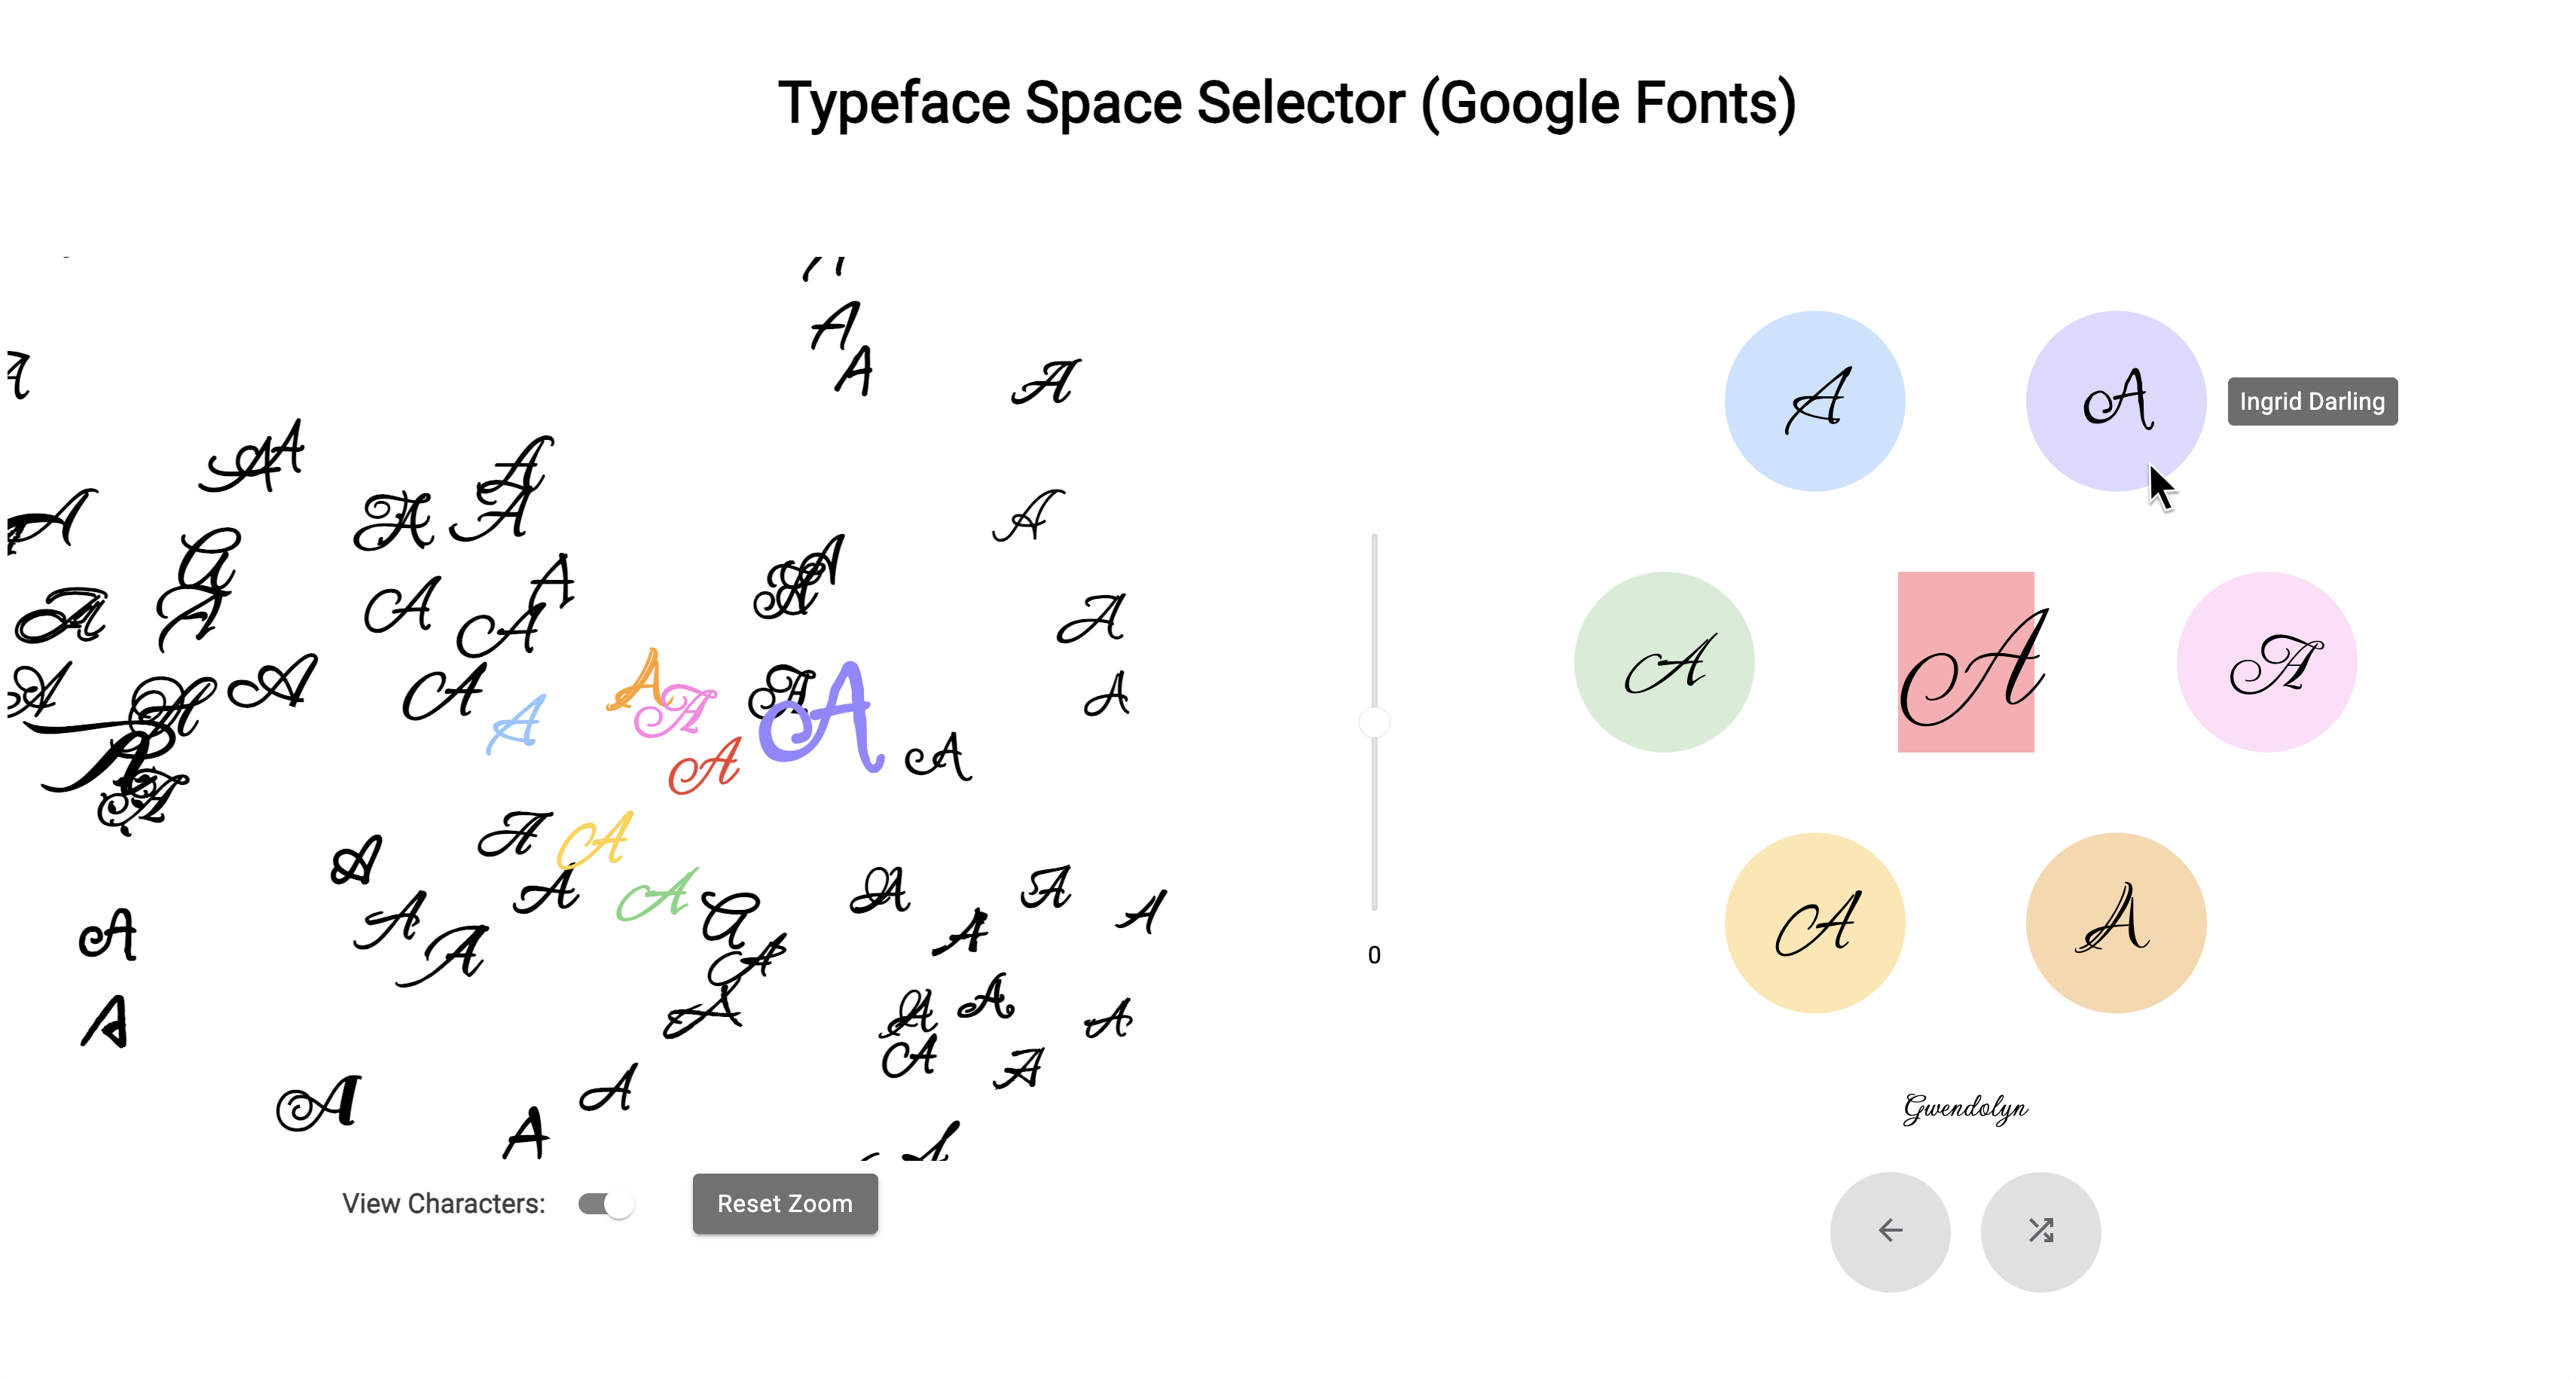
\includegraphics[width=\textwidth]{images/tool-with-chars.png}
    \caption{Our typeface selector tool with characters displayed on scatterplot, showing many nearby calligraphic fonts}
    \label{fig:tool-with-chars}
\end{figure}

In order to make our implementation more streamlined, this font selector is currently limited to the Google Fonts collection of typefaces. (This choice is described further in \ref{frontend}.) It would not be too difficult to expand support for fonts outside of the Google Fonts library, however it might require hosting SVG files of the font characters instead of loading full font files---which would become bulky and slow given a large number of fonts. (Consequently, this would likely speed up the tool's performance.) The current implementation of our font selector tool can be found here.\footnote{\url{http://sysnet.cs.williams.edu/~25sm39/}}

\subsection{Backend (Flask)}

We implement the backend of our web app in Flask,\footnote{\url{https://flask.palletsprojects.com/en/stable/}} a lightweight Python web server which adds expanded capability on top of the basic HTTP GET and POST requests and includes support for URL parameters, which we leverage to pass the magnitude data determining the server's nearest neighbors calculations. The backend server provides two functionalities. First, the backend serves the full t-SNE dataset for use in our scatterplot selector tool (a small file <1MB) upon request from the frontend web app. Second, the server can be queried to navigate the 6-dimensional model space and compute the nearest neighbor calculations necessary for the six-point font selector tool. Leveraging the Facebook AI Similarity Search (FAISS) library,\footnote{\url{https://ai.meta.com/tools/faiss/}} which provides efficient, high-dimensional vector similarity search, the backend first locates the style encoding for the input typeface, then computes six new style encoding vectors in each of the six dimensions according to the user-specified magnitude. FAISS then finds the nearest actual typeface style encoding for each of the six calculated vectors (see Figure \ref{fig:model-search}) avoiding duplicates when possible, and serves those font names to the client.

% my own figure
\begin{figure}[]
    \centering
    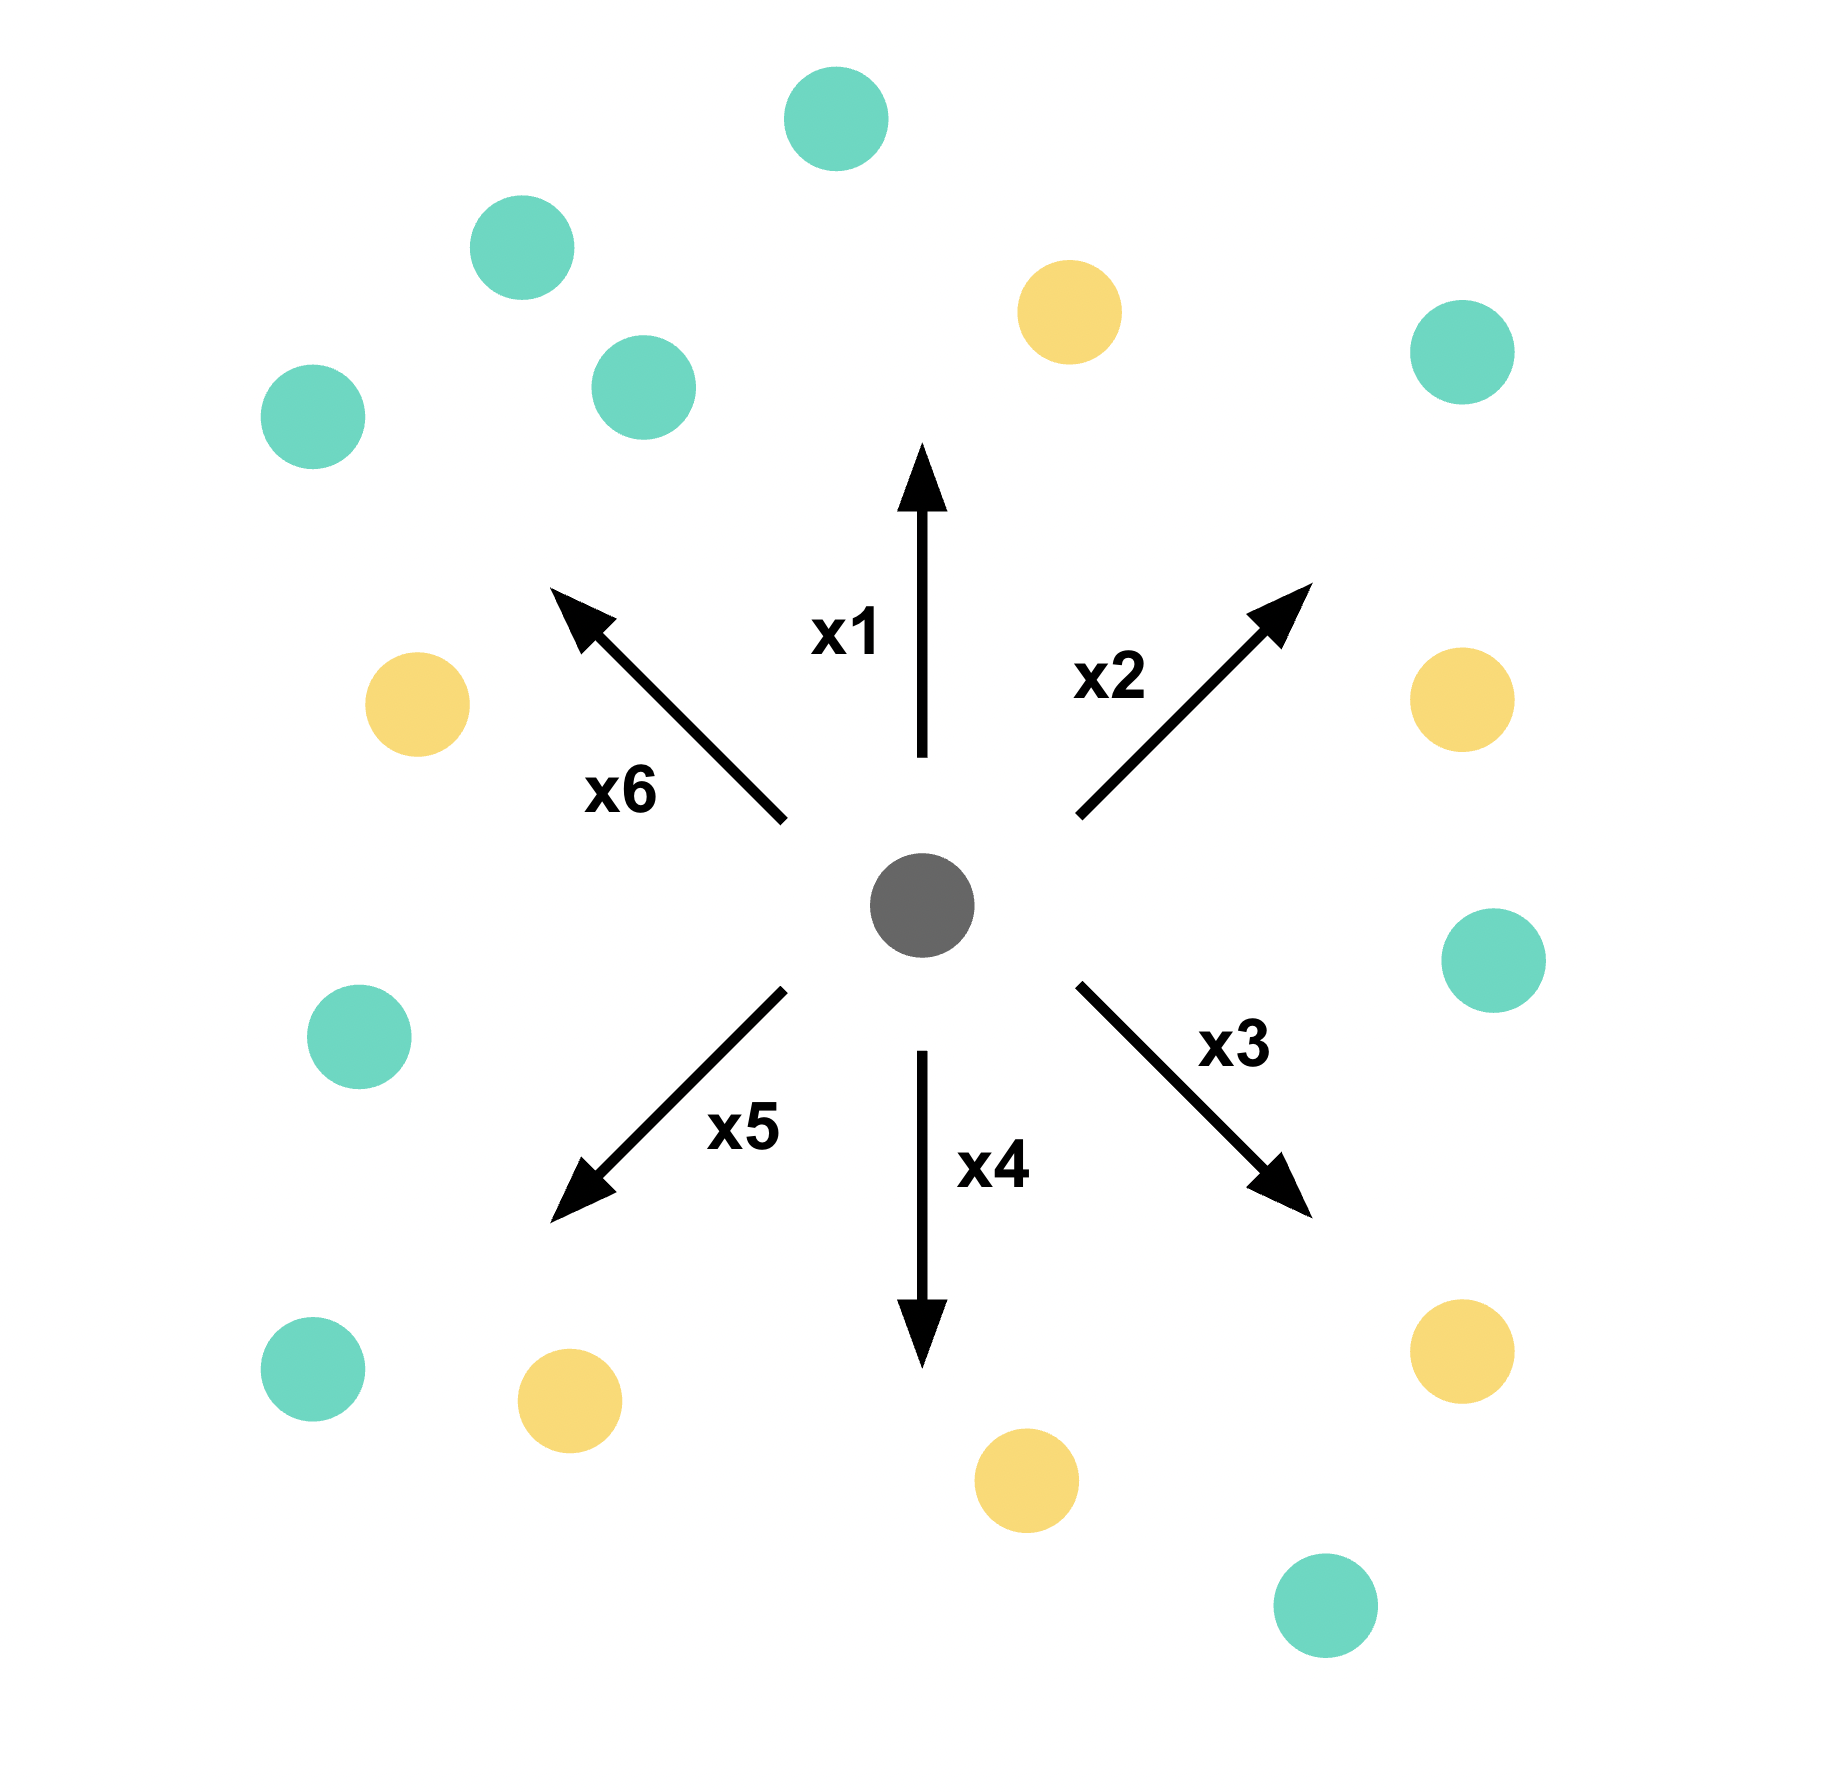
\includegraphics[width=0.55\textwidth]{images/model-search.png}
    \caption{Search algorithm in our model space: extend search in each dimension according to magnitude and find nearest neighbor}
    \label{fig:model-search}
\end{figure}

\subsection{Frontend (React)} \label{frontend}

Our frontend is implemented in React,\footnote{\url{https://react.dev/}} an open-source JavaScript library built to create interactive web applications using modular components. The scatterplot tool uses the Chart.js library\footnote{\url{https://www.chartjs.org/}} for simple, efficient plot creation, and the 6-point font selector was built using React components. For rendering the actual fonts, our frontend uses the GoogleFontLoader package for React,\footnote{\url{https://www.npmjs.com/package/react-google-font-loader}} which facilitates easy, dynamic font loading on webpages. This allows us to avoid serving the 2.7GB of font binary files, alleviating significant server load; however, it limits our current implementation to typefaces from the Google Fonts library. Although Google Fonts is widely-used and contains a wide range of different fonts, this does mean that common proprietary fonts such as Times New Roman and Comic Sans are not included in the current version of our font selector tool. A diagram of our system architecture can be found in Figure \ref{fig:system-diagram}.

% my own figure
\begin{figure}[]
    \centering
    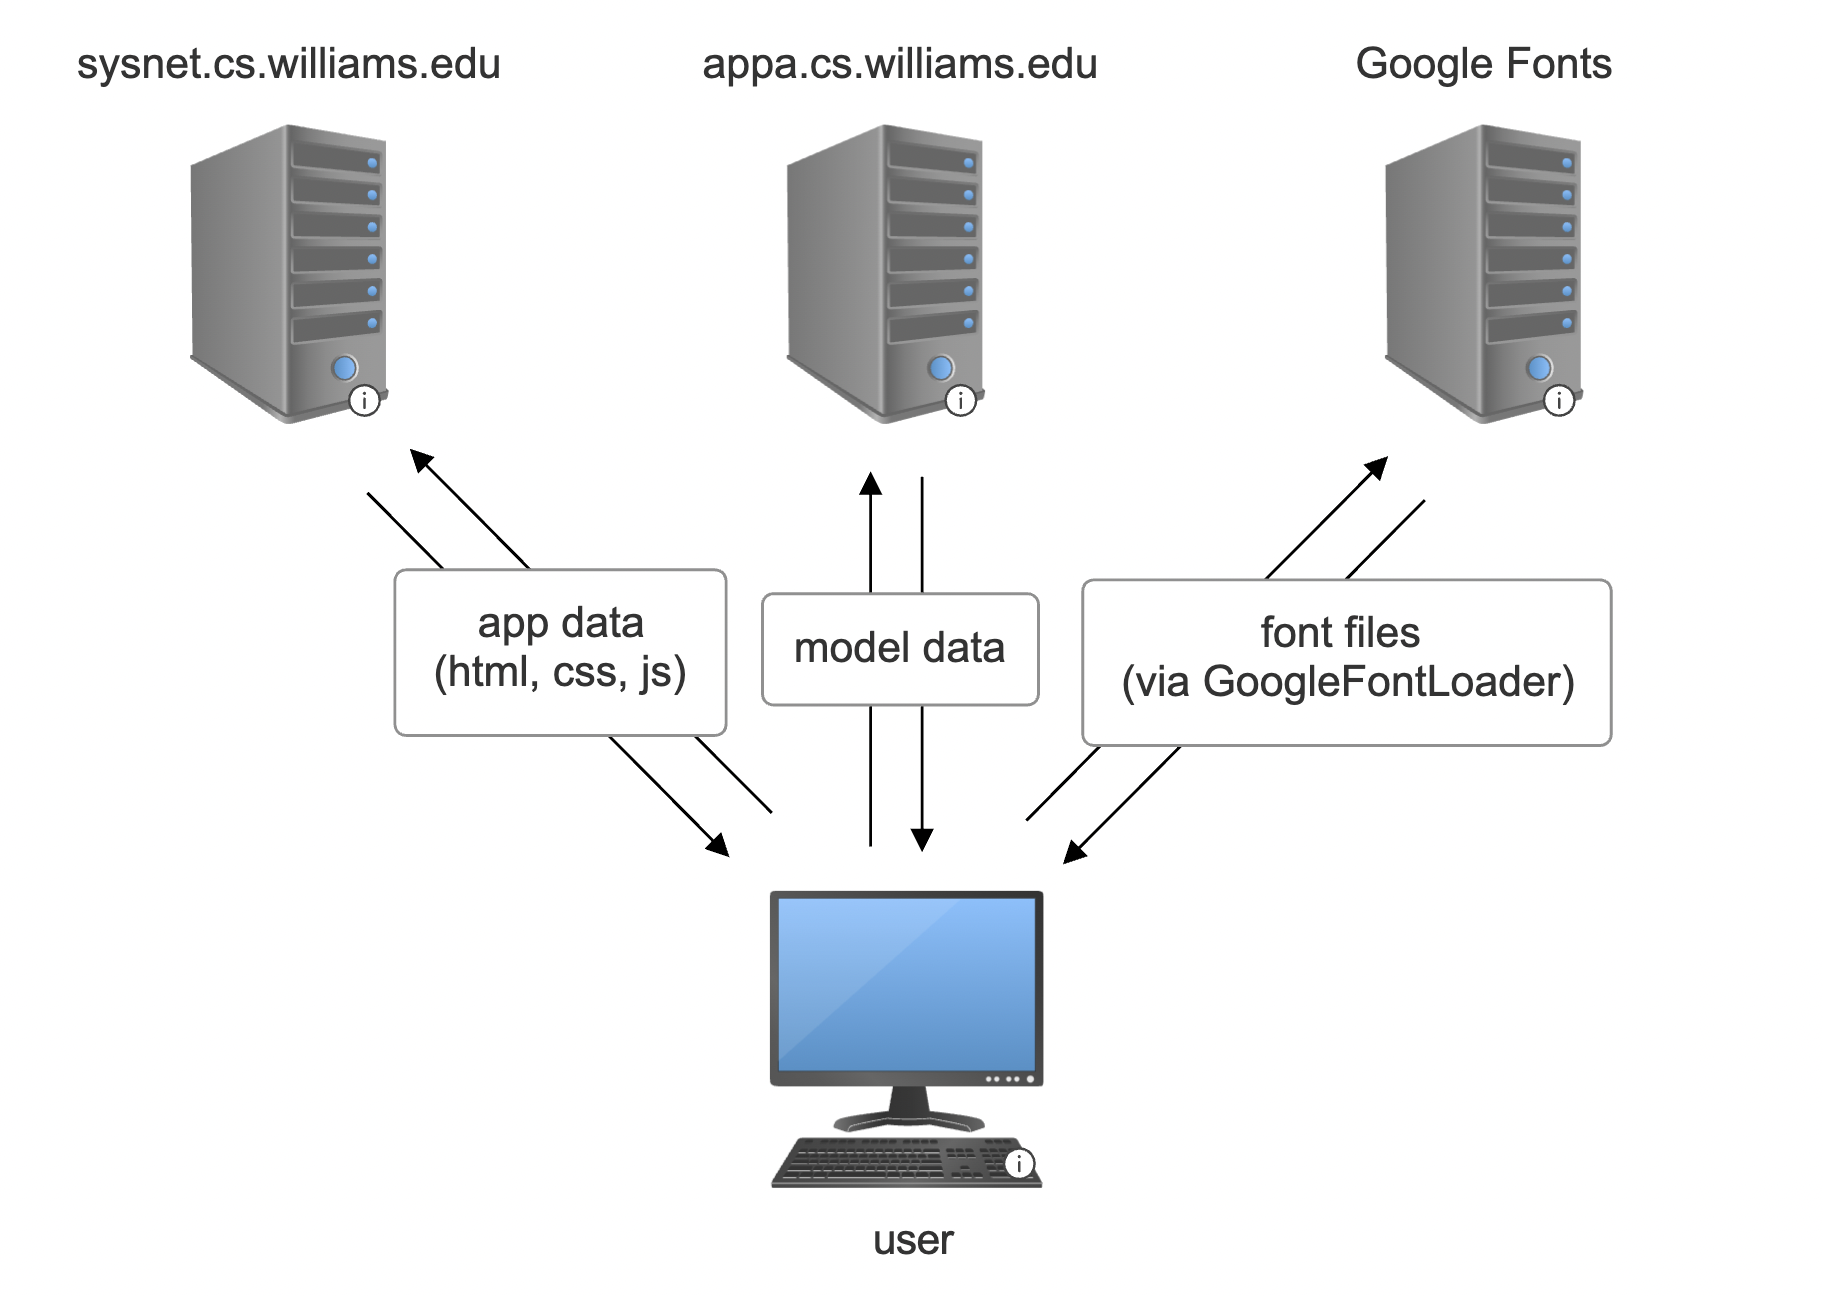
\includegraphics[width=0.9\textwidth]{images/system-diagram.png}
    \caption{A network diagram of our font selector web app system}
    \label{fig:system-diagram}
\end{figure}

\section{Accessing Code}

The full implementation of this project, including the backend server, the frontend webpage, and the training scripts for the models used to generate these style encodings, can be found in the GitHub repository referenced below.\footnote{\url{https://github.com/Mark-Hopkins-at-Williams/thesis-smagid}}
\chapter{Evaluation}
\label{chap:evaluation}

In this chapter we evaluate the performance of our model and novel font selection interface. Our Model Evaluation section includes a quantitative analysis of our model encodings, calculating the average pairwise distances of font groups in our model space according to the Google Fonts typeface categories discussed in Section \ref{font-selection-innovation}. In our User Evaluation section, we test our font selection interface against two alternate font selection tools with a small user study involving a font matching task and an open-ended qualitative evaluation. While the user evaluation certainly evaluates the usability and effectiveness of our selection interface, the model space itself---how accurately the model encodes typeface style---also affects the usability of the tool. Therefore, this user evaluation quantifies the combined effectiveness of the model encodings and the selector interface together.

\section{Model Evaluation} \label{model-eval}

We evaluate our models by measuring the average pairwise distances between fonts within each of the typeface style categories recently introduced by Google Fonts (see Section \ref{font-selection-innovation}), normalized against the overall average pairwise distance in the model space. While these categories are inherently subjective and have some inaccuracies (as previously discussed) they provide a useful grouping which is auxiliary to our model training and therefore can be used to evaluate our model encodings.

\begin{longtable}{|l|r|r|r|r|}
\caption{Average pairwise Euclidean distance between style encodings grouped by Google Fonts categories, normalized relative to the average pairwise distance between all fonts in model space. Abbreviated from Table \ref{tab:category-distances} (Appendix).}
\label{tab:category-distances-short} \\
\hline
\textbf{Category} & \textbf{Autoencoder} & \textbf{Style Transfer} & \textbf{Sriv. C64} & \textbf{Sriv. Full} \\
\hhline{|=====|}
average category distance & 1.318 & 1.337 & \textbf{0.952} & \textbf{0.769} \\
\# beat average? & 23 & 21 & 39 & 65 \\
\hhline{|=====|}
\endfirsthead

\multicolumn{5}{c}{{Table \thetable\ continued from previous page}} \\[0.5em]
\hline
\textbf{Category} & \textbf{Autoencoder} & \textbf{Style Transfer} & \textbf{Sriv. C64} & \textbf{Sriv. Full} \\
\hline
\endhead

\hline \multicolumn{5}{r}{{Continued on next page}} \\
\endfoot

\hline
\endlastfoot

appearance-art-deco       & 1.728          & 1.337          & 1.184          & \textbf{0.780} \\
appearance-art-nouveau    & \textbf{0.453} & \textbf{0.737} & \textbf{0.783} & \textbf{0.706} \\
appearance-blackletter    & \textbf{0.698} & \textbf{0.956} & \textbf{0.956} & \textbf{0.921} \\
appearance-blobby         & 1.198          & 1.276          & \textbf{0.880} & \textbf{0.657} \\
appearance-distressed     & 1.489          & 1.278          & 1.057          & \textbf{0.698} \\
appearance-inline         & 2.238          & 1.832          & 1.209          & \textbf{0.732} \\
\hline
\multicolumn{5}{|c|}{$\cdots$} \\
\hline
serif-fatface             & 2.478          & 2.896          & 1.082          & \textbf{0.755} \\
serif-humanist            & \textbf{0.628} & \textbf{0.545} & \textbf{0.873} & \textbf{0.841} \\
serif-modern              & \textbf{0.794} & \textbf{0.596} & \textbf{0.847} & \textbf{0.889} \\
serif-old-style           & \textbf{0.522} & \textbf{0.753} & \textbf{0.695} & \textbf{0.814} \\
serif-slab                & 1.582          & 1.347          & 1.117          & \textbf{0.845} \\
serif-transitional        & \textbf{0.551} & \textbf{0.667} & \textbf{0.732} & \textbf{0.954} \\

\end{longtable}

Table \ref{tab:category-distances-short} displays representative results from this evaluation. Each row contains data for a different Google Fonts category, and the four columns represent our four models. (\textbf{Sriv. C64} is the Srivatsan model trained only on the Capitals64 dataset, while \textbf{Sriv. Full} is the Srivatsan model trained on our full dataset.) We find that the Srivatsan model, trained on the smaller Capitals64 dataset, outperforms both the Autoencoder and Style Transfer models, with a greater number of Google Fonts categories having a lower average distance between fonts than the overall pairwise average ($n=39$), and the average distance score across all the categories slightly lower than the overall average (0.952). However, when trained on our full dataset---including Capitals64, Google Fonts, and preinstalled fonts from macos---the Srivatsan model performs even better, with 65 of the Google Font categories having a closer-than-average distance score---all but one---and an average distance score across all the categories of 0.769, much lower than the average pairwise encoding distance.

It makes sense that the Srivatsan model would perform better with our full dataset: partially, this may be due to simply having a larger, more representative training dataset; but this is also likely a result of having seen the Google Fonts in its training. In the latter instance, the Srivatsan model was able to actively optimize the style encodings for the Google Fonts typefaces, while the more limited Srivatsan model did not have the opportunity to specifically optimize these style encodings. This does not, however, mean that the Google Fonts style encodings of the full Srivatsan model are of lower quality; rather, having the ability to specifically train on these fonts should result in better, more accurate style encodings for use in our font selection tool.

Looking at the extended data in Table \ref{tab:category-distances} (Appendix), we can also make some conclusions about the different models' abilities to encode certain types of style. For example, we find that all model implementations encode sans-serif style quite effectively, as the average distance scores for most of the sans-serif style groups are lower than the overall average distance in their model spaces. The same is true for most of the serif style groups; however, only the fully trained Srivatsan model seems capable of encoding the style of the serif-fatface and serif-slab groups. This makes some sense, as these two categories contain less typical serif style fonts (see Figures \ref{fig:serif-fatface} and \ref{fig:serif-slab}), but the groups are also relatively small (15 and 68 fonts, respectively) and it is hard to make a definite conclusion with such a small sample size.

% my own figure
\begin{figure}[]
    \centering
    
\includegraphics[width=\textwidth]{images/serif-fatface.png}
    \caption{Selection of fonts in the Google Fonts serif-fatface category}
    \label{fig:serif-fatface}
\end{figure}

% my own figure
\begin{figure}[]
    \centering
    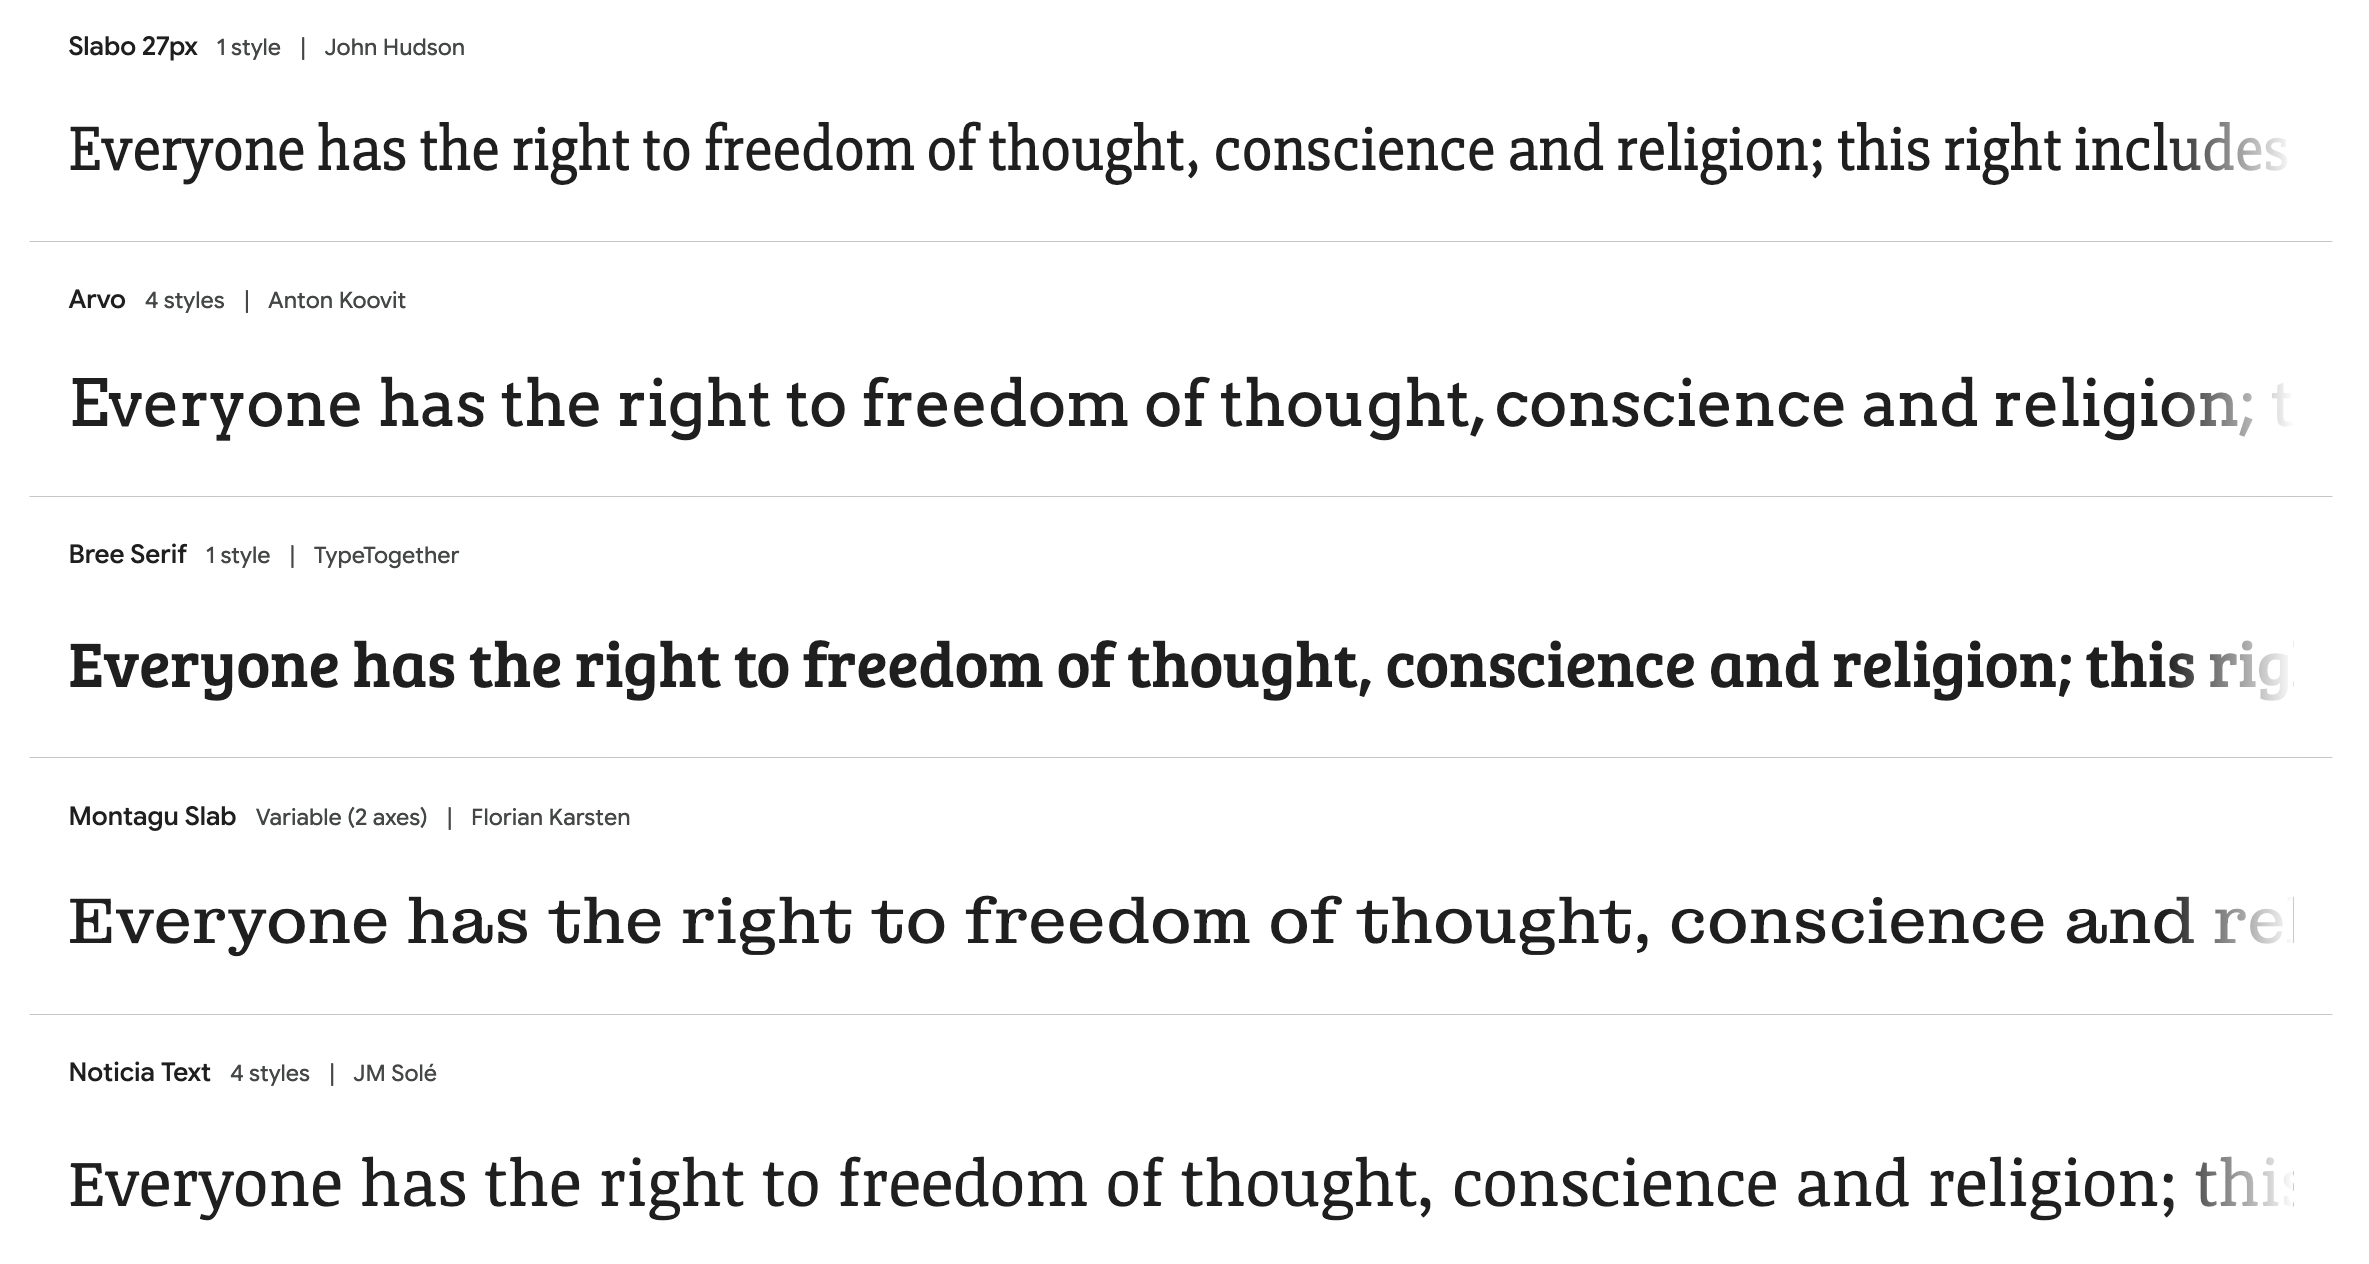
\includegraphics[width=\textwidth]{images/serif-slab.png}
    \caption{Selection of fonts in the Google Fonts serif-slab category}
    \label{fig:serif-slab}
\end{figure}

% my own figure
\begin{figure}[]
    \centering
    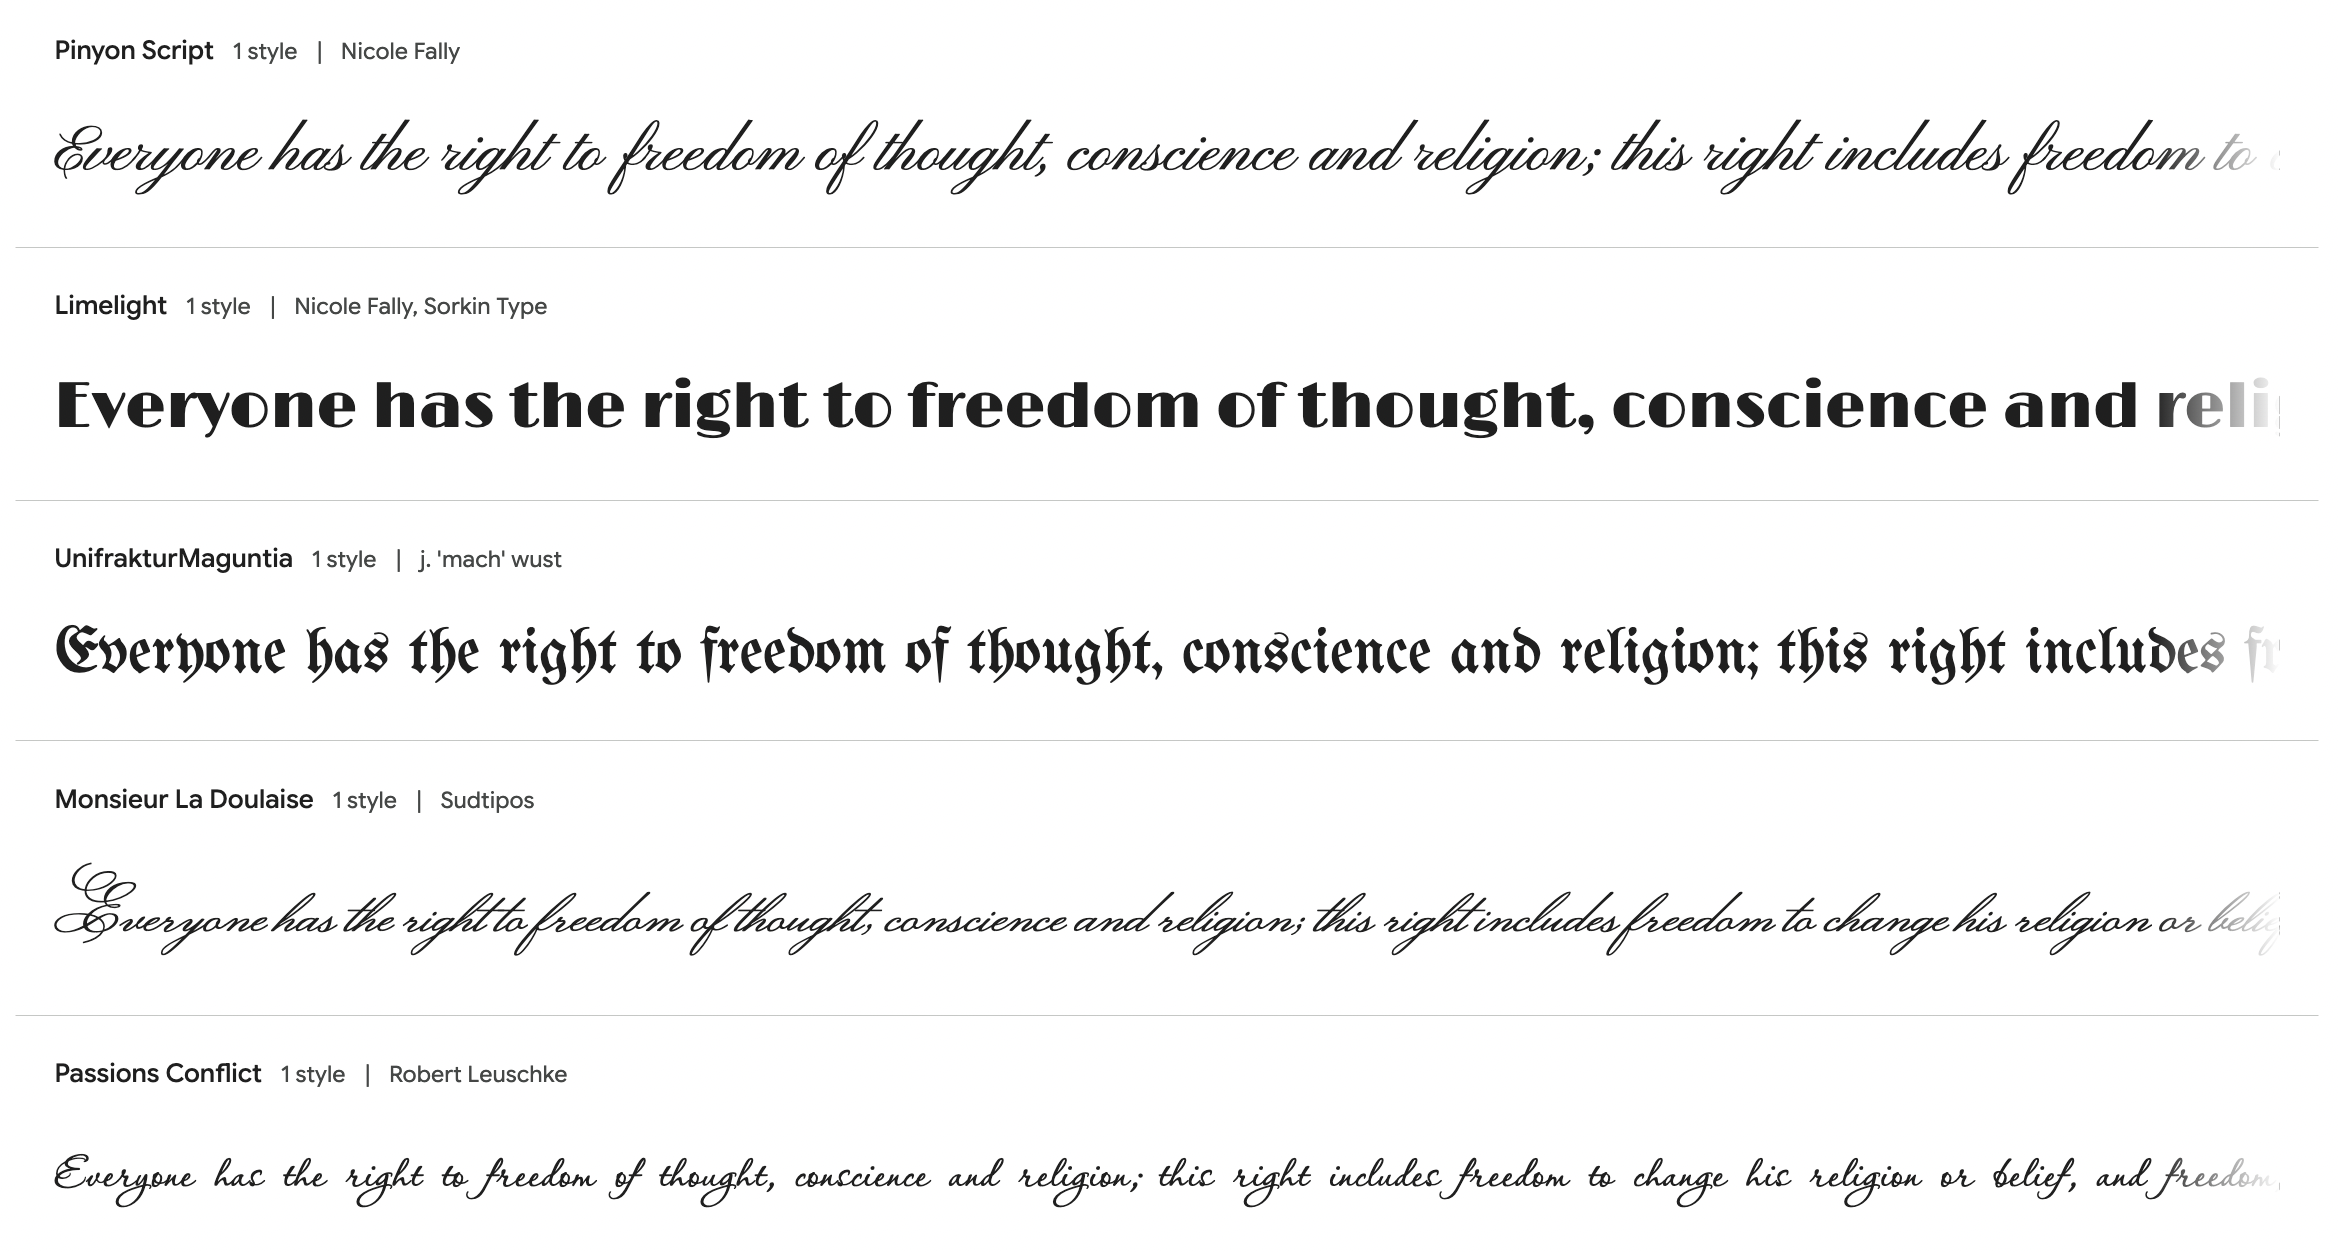
\includegraphics[width=\textwidth]{images/feeling-artistic.png}
    \caption{Selection of fonts in the Google Fonts feeling-artistic category}
    \label{fig:feeling-artistic}
\end{figure}

% my own figure
\begin{figure}[]
    \centering
    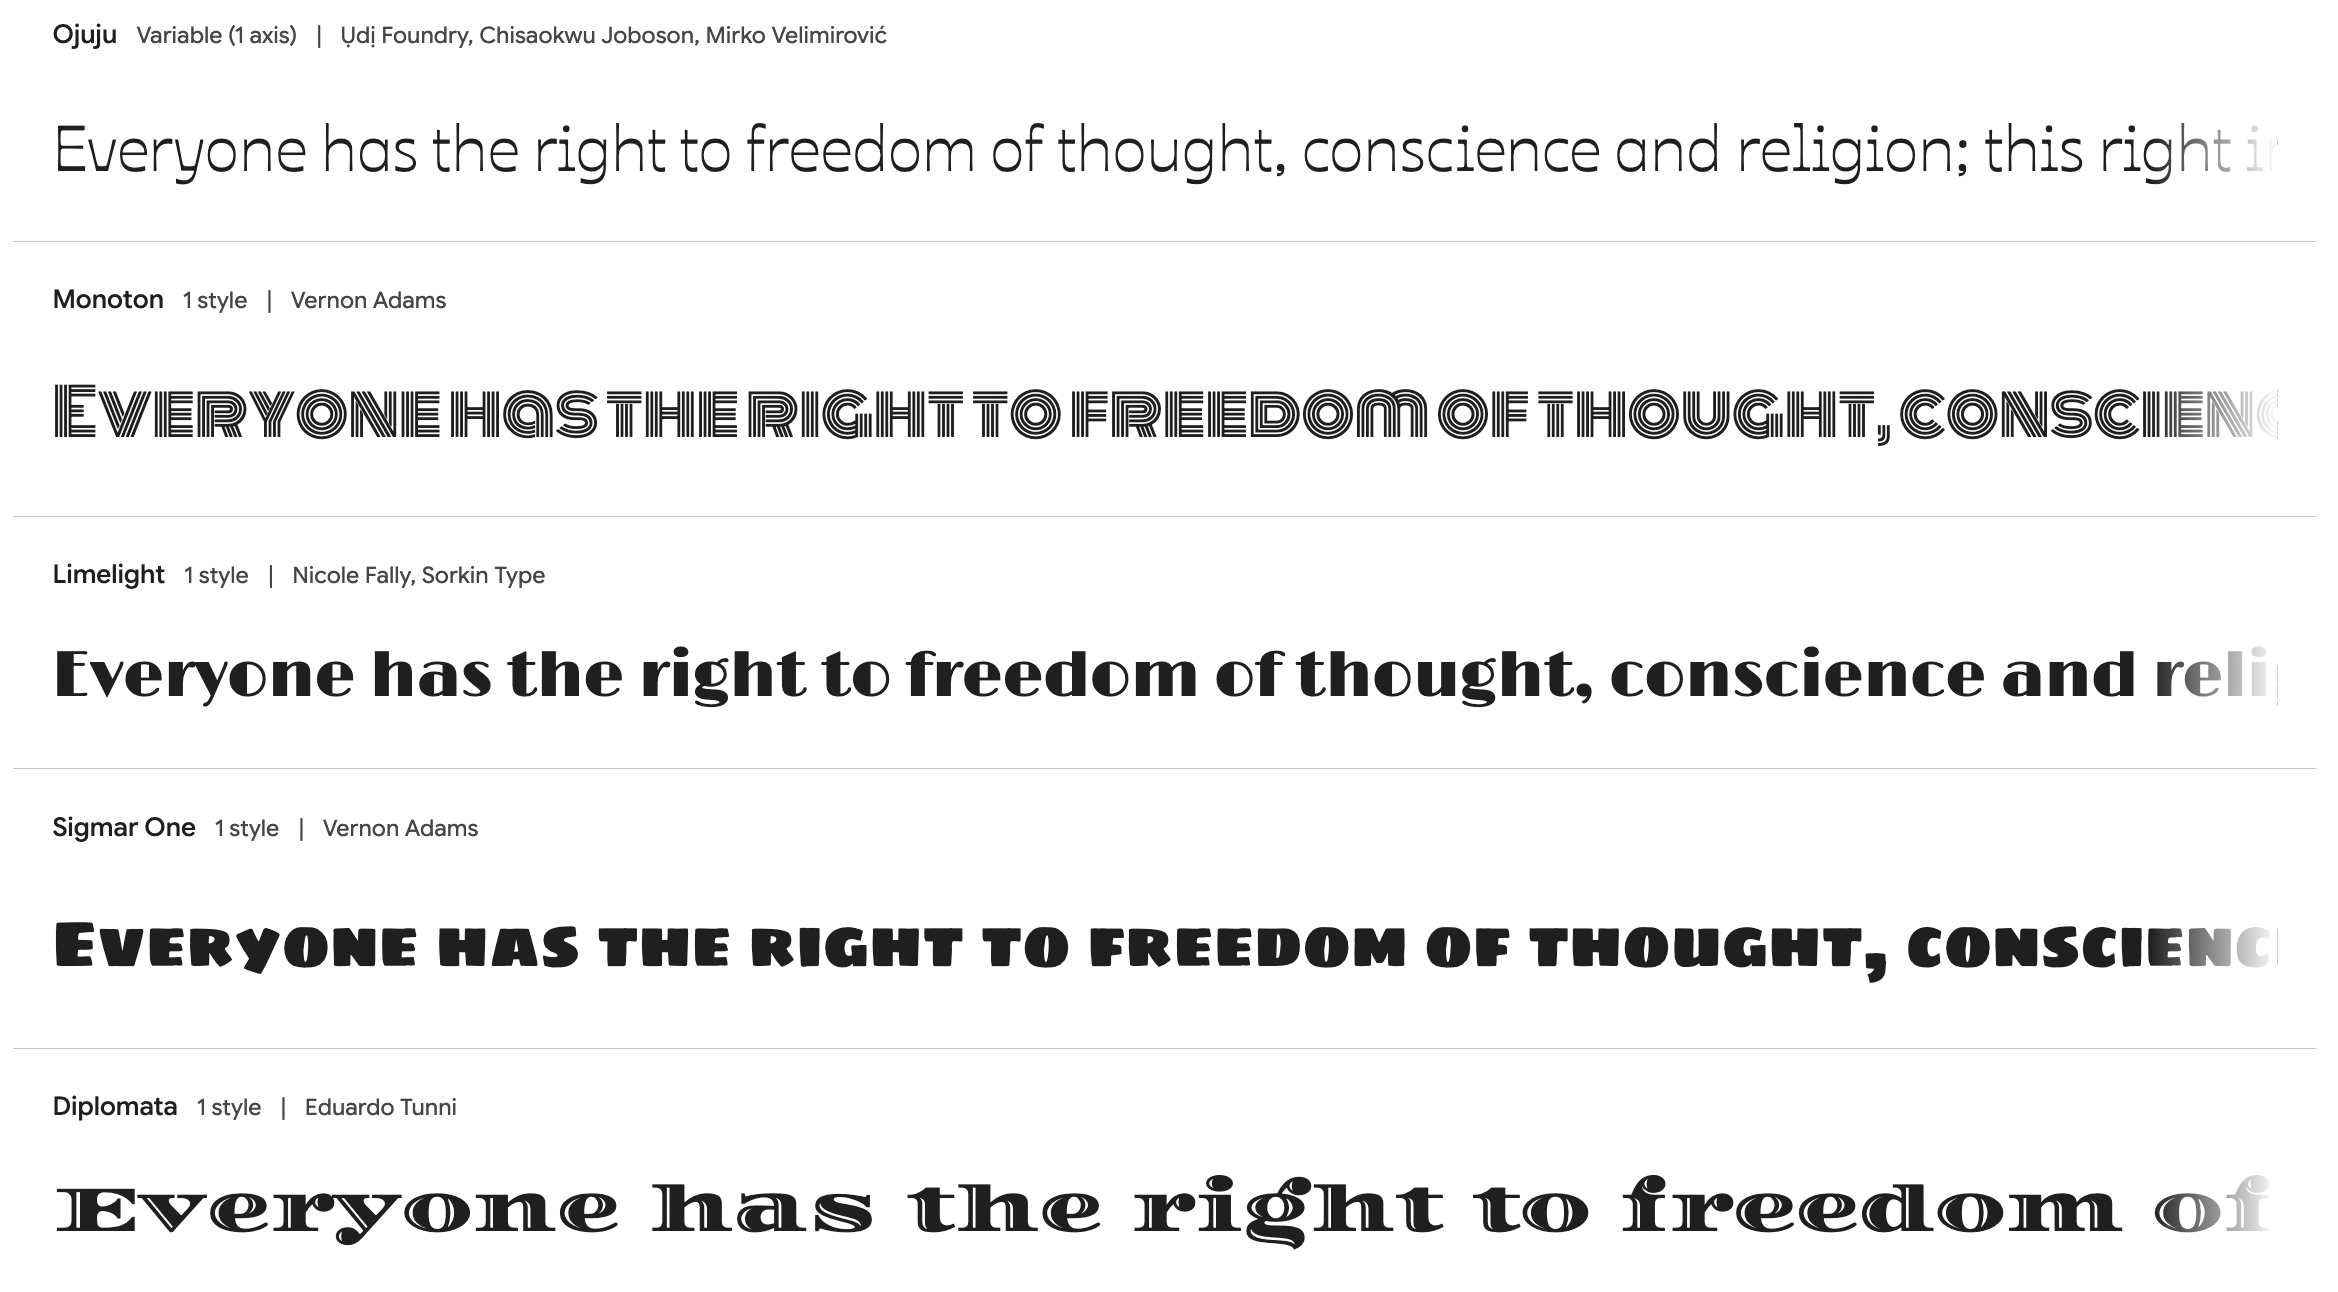
\includegraphics[width=\textwidth]{images/seasonal-kwanzaa.png}
    \caption{Selection of fonts in the Google Fonts seasonal-kwanzaa category}
    \label{fig:seasonal-kwanzaa}
\end{figure}

We additionally find that some of the more ambiguous font style categories are not well-encoded by our simpler models. In particular, style categories in the appearance, feeling, and seasonal groups have low average similarity scores in the encoding spaces of the more basic models. For many of these ambiguous style categories, only the Srivatsan model trained on our full dataset seemed to recognize the implicit connections among their fonts. Many of these ambiguous stylistic categories contain a wide variety of different font styles, making it difficult to explicitly identify their common traits. For example, the fonts in the feeling-artistic and seasonal-kwanzaa categories (see Figures \ref{fig:feeling-artistic} and \ref{fig:seasonal-kwanzaa}) do not seem to follow one particular or obvious style. Somewhat surprisingly, our final model recognizes common threads among fonts even in these more abstract style groups, suggesting that these model encodings should provide a strong foundation for style-based font selection.

\subsection{A Note: Euclidean Distance vs Cosine Similarity}

We find an interesting result when comparing the cosine and Euclidean distances in our model evaluation. In general, we find that the models which perform strongly for Euclidean distance do not perform as well when considering cosine similarity; and conversely, the models which perform less well in terms of Euclidean closeness perform better with cosine similarity. For example, when comparing the normalized category-wise Euclidean distances and cosine similarities of the Autoencoder model (see Table \ref{tab:euclidean-vs-cosine-auto-short}), we find that a greater number of categories have a better-than-average similarity when considering cosine similarity ($n=41$) rather than Euclidean distance ($n=23$); and the average similarity score across all category groups is closer than average (1.125) as measured by cosine similarity but further than average (1.318) when using Euclidean distance. On the other hand, our full Srivatsan model performs very well on Euclidean distance scores but not as well when using cosine similarity (see Table \ref{tab:euclidean-vs-cosine-sriv-short}), with far fewer scores beating the average under the cosine similarity metric ($n=36$) and the average category-wise cosine similarity score (0.987) slightly worse than the overall pairwise average for the full model space. It is unclear exactly why there is a discrepancy with cosine and Euclidean similarity evaluation in our model space---it is certainly the case that Euclidean and cosine similarity metrics are measuring different types of vector similarity, which might be representing different aspects of the model encodings---but for the purposes of our selection tool this should not matter: since our user tool is built around Euclidean distance metrics, it is mainly important that our full Srivatsan model performs well under Euclidean distance metrics---that similar font styles should be closer to each other in Euclidean space---which it does. Cosine similarity metrics tell an interesting story about our model space, but ultimately the metric of most importance for our purposes is Euclidean distance.

\begin{longtable}{|l|r|r|}
\caption{Normalized average pairwise Euclidean and cosine distances across Google Fonts category groups in our Autoencoder model space. Abbreviated from Table \ref{tab:euclidean-vs-cosine-auto} (Appendix).}
\label{tab:euclidean-vs-cosine-auto-short} \\
\hline
\textbf{Category} & \textbf{Autoencoder (Euclidean)} & \textbf{Autoencoder (Cosine)} \\
\hhline{|===|}
average category distance & 1.318 & \textbf{1.125} \\
\# beat average? & 23 & 41 \\
\hhline{|===|}
\endfirsthead

\multicolumn{3}{c}{{Table \thetable\ continued from previous page}} \\[0.5em]
\hline
\textbf{Category} & \textbf{Autoencoder (Euclidean)} & \textbf{Autoencoder (Cosine)} \\
\hline
\endhead

\hline \multicolumn{3}{r}{{Continued on next page}} \\
\endfoot

\hline
\endlastfoot

appearance-art-deco       & 1.728                   & \textbf{1.282}      \\
appearance-art-nouveau    & \textbf{0.453}          & 0.494               \\
appearance-blackletter    & \textbf{0.698}          & \textbf{1.101}      \\
appearance-blobby         & 1.198                   & 0.906               \\
appearance-distressed     & 1.489                   & \textbf{1.434}      \\
appearance-inline         & 2.238                   & \textbf{1.692}      \\
appearance-lunar-new-year & 1.390                   & \textbf{1.742}      \\
appearance-marker         & 1.139                   & \textbf{1.045}      \\
appearance-medieval       & \textbf{0.934}          & 0.848               \\
appearance-monospaced     & \textbf{0.475}          & 0.866               \\
appearance-not-text       & 6.477                   & \textbf{2.699}      \\
\hline
\multicolumn{3}{|c|}{$\cdots$} \\
\hline
serif-didone              & 1.238                   & 0.853               \\
serif-fatface             & 2.478                   & 0.666               \\
serif-humanist            & \textbf{0.628}          & 0.535               \\
serif-modern              & \textbf{0.794}          & 0.955               \\
serif-old-style           & \textbf{0.522}          & 0.544               \\
serif-scotch              & \textbf{0.562}          & 0.808               \\
serif-slab                & 1.582                   & 0.920               \\
serif-transitional        & 0.551                   & 0.529         \\           

\end{longtable}

\begin{longtable}{|l|r|r|}
\caption{Normalized average pairwise Euclidean and cosine distances across Google Fonts category groups in our full Srivatsan model space. Abbreviated from Table \ref{tab:euclidean-vs-cosine-sriv} (Appendix).}
\label{tab:euclidean-vs-cosine-sriv-short} \\
\hline
\textbf{Category} & \textbf{Srivatsan Full (Euclidean)} & \textbf{Srivatsan Full (Cosine)} \\
\hhline{|===|}
average category distance & \textbf{0.769} & 0.987 \\
\# beat average? & 65 & 36 \\
\hhline{|===|}
\endfirsthead

\multicolumn{3}{c}{{Table \thetable\ continued from previous page}} \\[0.5em]
\hline
\textbf{Category} & \textbf{Srivatsan Full (Euclidean)} & \textbf{Srivatsan Full (Cosine)} \\
\hline
\endhead

\hline \multicolumn{3}{r}{{Continued on next page}} \\
\endfoot

\hline
\endlastfoot

appearance-art-deco       & \textbf{0.780}             & \textbf{1.266}          \\
appearance-art-nouveau    & \textbf{0.706}             & 0.650                   \\
appearance-blackletter    & \textbf{0.921}             & 0.881                   \\
appearance-blobby         & \textbf{0.657}             & 0.955                   \\
appearance-distressed     & \textbf{0.698}             & \textbf{1.303}          \\
appearance-inline         & \textbf{0.732}             & \textbf{1.140}          \\
appearance-lunar-new-year & \textbf{0.841}             & \textbf{1.264}          \\
appearance-marker         & \textbf{0.651}             & \textbf{1.104}          \\
appearance-medieval       & \textbf{0.758}             & 0.855                   \\
appearance-monospaced     & \textbf{0.746}             & 0.909                   \\
appearance-not-text       & \textbf{0.754}             & \textbf{1.707}          \\
\hline
\multicolumn{3}{|c|}{$\cdots$} \\
\hline
serif-humanist            & \textbf{0.841}             & 0.525                   \\
serif-modern              & \textbf{0.889}             & 0.597                   \\
serif-old-style           & \textbf{0.814}             & 0.477                   \\
serif-scotch              & \textbf{0.891}             & 0.502                   \\
serif-slab                & \textbf{0.845}             & 0.849                   \\
serif-transitional        & \textbf{0.954}             & 0.468              

\end{longtable}

\section{User Evaluation} \label{user-eval}

% my own figure
\begin{figure}[h]
    \centering
    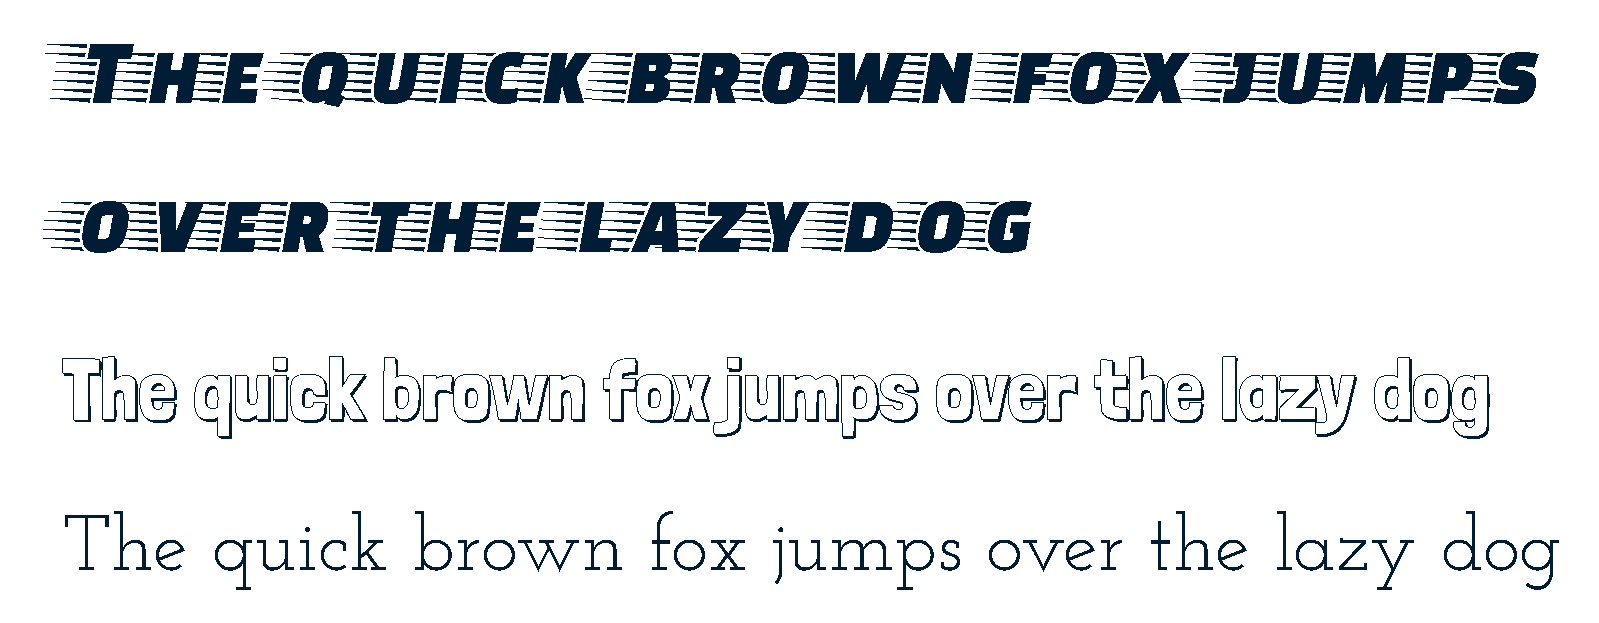
\includegraphics[width=\textwidth]{images/user-fonts.pdf}
    \caption{Fonts chosen for our user study (Faster One, Londrina Shadow, and Josefin Slab, from top to bottom) with sample text ``The quick brown fox jumped over the lazy dog''}
    \label{fig:user-fonts}
\end{figure}

We additionally conducted a small user study to qualify the effectiveness of our font selection interface. 12 participants were each given three fonts (on a printed piece of paper) and three corresponding font identification tasks using each of three interfaces: the basic list-based font selector in Google Docs, the category-based search from Google Fonts, and our typeface-space selector. We chose three fonts which would represent a variety of search difficulties: one which was very distinct and would not be confused with another typeface in our set (Faster One), another which was somewhat distinct but has some lookalike fonts in the set (Londrina Shadow), and third which was more generic and likely harder to find among similar fonts (Josefin Slab). For each user, we presented one of the three fonts showing a default display text (see Figure \ref{fig:user-fonts}) and introduced one of the tools, then gave the participant two minutes to try and identify the font using the given tool. We repeated the task two additional times, randomizing the order of tools between participants, so that each user tried all three tools and attempted to identify each font. By randomizing tool order but keeping font order the same, we ensured that our performance data would not be affected by the choice of font. We kept track of several pieces of data: remaining time (if the user selected a font in less than two minutes); \# of clicks, mouse movements, and scrolls; and also the selected font, which we used to calculate the normalized Euclidean distance from the correct font in our space (i.e. how close the user got, zero if correct).

\begin{longtable}{|l|r|r|r|r|r|r|}
\caption{Quantitative results from font matching user study, averaged across trials, with distance from correct normalized to average pairwise distance in encoding space.}
\label{tab:user-study-quant} \\
\hline
\textbf{selector} & \textbf{\% correct} & \textbf{distance} & \textbf{time left} & \textbf{clicks} & \textbf{scrolls} & \textbf{mouse moves} \\
\hline
\endfirsthead

\multicolumn{3}{c}{{Table \thetable\ continued from previous page}} \\[0.5em]
\hline
\textbf{selector} & \textbf{\% correct} & \textbf{distance} & \textbf{time left} & \textbf{clicks} & \textbf{scrolls} & \textbf{mouse moves} \\
\hline
\endhead

\hline \multicolumn{3}{r}{{Continued on next page}} \\
\endfoot

\hline
\endlastfoot

list & 0.5 & 0.353 & 0:30 & 8.9 & 72 & 60.4 \\
google fonts & 0.67 & 0.291 & 0:29 & 16.2 & 62.5 & 78.9 \\
our tool & 0.55 & 0.359 & 0:39 & 23.6 & 2.9 & 112.6                 

\end{longtable}

Given the small size of our user study ($n=12$) and the many possible sources of noise in our trial, it is difficult to draw many significant conclusions from our data. For example, it appears as though users chose slightly closer-to-correct fonts (according to the Euclidean distance metric in our encoding space) when using the Google Fonts selector---and were also more often correct in their selection---but given the closeness of these numbers and the high amount of variation in our data, we cannot substantially differentiate these performances. The data that appear most significant are our measures of clicks, scrolls, and mouse moves: unsurprisingly, users tended to scroll more on the basic list and Google Fonts selectors---which are both scroll-based interfaces---and tended to use more mouse moves on our tool, which relies on mouse movements for most of its selection mechanisms. While the study was too small to draw very significant conclusions about accuracy performance, it is useful to explore methods for quantifying font selection tools and begin to understand the usefulness of our tool. Importantly, a font matching task may not be the best method to evaluate tool performance, as oftentimes in real-world use scenarios, users do not seek to match an exact font but rather to explore several fonts and find a desireable one. O'Donovan et al. \cite{odonovan2014}, for example, utilize two tasks in their font selection tool evaluation: a font matching task similar to ours, and also a more subjective task asking to find a ``good'' font for the design of a given document.

At the end of each trial, we also asked users to qualitatively evaluate each of the tools. For each selector, we simply asked the user to list positive and negative aspects of each tool---what they liked, didn't like, found helpful, or not. These results are helpful in both evaluating our own tool and better understanding user needs in font selection tasks. Table \ref{tab:user-study-qual} shows a summary of user responses, organized by ``advantages'' and ``disadvantages'' of each tool. For the basic list interface, we received the same piece of feedback from most users: that alphabetical order is not useful when selecting fonts based on style, and the lack of categories led to a long, mundane search experience. Additionally, users reported finding the small text size difficult and found it frustrating that the tool did not save their place in the long list when they clicked away from it. However, users did find the simplicity of the interface useful, as well as the fact that it displays many characters at once in the font name. For the Google Fonts category-search interface, users liked the ability to search by attribute, but they found that the categories were often too vague or subjective; additionally, sometimes a category they envisioned and hoped to use (e.g. ``Block Letters'') was not an available option. For our style-based tool, users liked that the interface tended to cluster fonts by similarity, allowing them to narrow down their search and eliminate parts of the map from consideration, and generally found the interface to be fun and explorative; however, many found the tool somewhat unintuitive and difficult to use at first, wished they could preview more letters at once, and were frustrated by the lag which occurs due to character re-rendering when zooming in the map tool.

\begin{longtable}{|l|l|l|}
\caption{Summary of qualitative results from user study, separated into ``advantages'' and ``disadvantages'' of each tool.}
\label{tab:user-study-qual} \\
\hline
& \textbf{advantages} & \textbf{disadvantages} \\
\hline
\endfirsthead

\multicolumn{3}{c}{{Table \thetable\ continued from previous page}} \\[0.5em]
\hline
& \textbf{advantages} & \textbf{disadvantages} \\
\hline
\endhead

\hline \multicolumn{3}{r}{{Continued on next page}} \\
\endfoot

\hline
\endlastfoot

list &

\begin{tabular}[c]{@{}l@{}}
simple interface\\
helpful if you know the name already\\
ability to save fonts\\
displays many letters for each font
\end{tabular} &

\begin{tabular}[c]{@{}l@{}}
no style-based search\\
alphabetic order is not useful\\
too much to scroll through\\
doesn't save your place\\
small text\\
boring
\end{tabular} \\

google fonts &

\begin{tabular}[c]{@{}l@{}}
ability to preview text\\
search by attribute\\
ability to narrow down search
\end{tabular} &

\begin{tabular}[c]{@{}l@{}}
categories are subjective and often vague\\
too many categories\\
some categories did not exist\\
no open-ended descriptor search
\end{tabular}\\

\hline

our tool &

\begin{tabular}[c]{@{}l@{}}
ability to narrow down search\\
clustered by similarity\\
ability to eliminate areas of map from\\
search based on style\\
playful interface\\
fun to explore
\end{tabular} &

\begin{tabular}[c]{@{}l@{}}
difficult to understand many features\\
dimensional aspect unclear\\
font not always where expected\\
only able to display one letter\\
lag with character rendering\\
no text-based search feature
\end{tabular} \\

\end{longtable}

These qualitative data are useful in understanding how users make use of our tool and evaluating it against other existing font selection interfaces. For example, there was a clear sentiment, expressed by almost all of our participants, that the basic list selector was limited by not including any aspect of style or stylistic categories in its interface. Users tended to like the Google Fonts category search, but the subjectivity of categories was a limiting factor. Our style-encoding search represents a very different method of font selection: one based on trained, quantitative stylistic model encodings. While our tool was somewhat unintuitive for some first-time users, it was nonetheless received well as a fun and useful style-based font exploration tool. Some improvements would be necessary to make this into a finalized user-ready tool, but this proof-of-concept font selection interface suggests that the style encodings produced by autoencoder-like neural networks can certainly be used to create useful style-based typeface selection tools.
\chapter{Conclusion}
\label{chap:conclusion}

In this thesis, we have detailed our research into the potential use of autoencoder-like neural networks to encode typeface style. The most common font selection tools largely ignore style as an aspect of typeface selection, making it difficult or impossible to ask questions like ``Which fonts are most similar to Futura?'' or ``What is a font which is similar to Times New Roman but more playful?'' The first half of our research involved gathering a large dataset of font character data representative of a wide range of typeface styles, including character sets from 14,391 typefaces across the Google Fonts and Apple libraries and the Capitals64 dataset (see Section \ref{data-collection}), and training several models based on the original autoencoder model to encode typeface style vectors of input character sets. The second half of this project involved building a useful proof-of-concept user tool on these typeface style encoding data, in order to demonstrate our hypothesis that the style encodings generated by these autoencoder-based neural networks can serve as a useful foundation for style-based font selection. Finally, we quantitatively evaluated the stylistic encoding space produced by our models, and additionally performed a small user study to both quantitatively and qualitatively evaluate the performance of our font selection tool.

\section{Findings}

We find that many of our models succeed in encoding certain aspects typeface style, but our model adapted from Srivatsan et al. \cite{srivatsan2020} and trained on our larger dataset---including the fonts from Google Fonts, Apple, and Capitals64---performed the strongest when evaluated against the novel font attribute categories created by the Google Fonts library: when looking at Euclidean distance as a metric of style vector similarity, all but one of the Google Fonts style categories corresponded to a closer-than-average Euclidean similarity score. The other models captured fewer of these categories, and we generally find that models which were more complex and disentangled character structure (A or B, e.g.) from style (determined by typeface) performed better on these Euclidean similarity metrics. In general, ``easier'' style categories---such as serif and sans-serif category groups---were more likely to have a closer-than-average similarity score across the models, while more abstract and diverse style categories like feeling-loud or seasonal-kwanzaa were less likely to have closer-than-average distance scores. We also measured these similarity scores using cosine similarity distances, and found that the cosine similarity metric told a somewhat different story than Euclidean distance similarity---the models which performed better under Euclidean distance similarity tended to perform poorer under cosine similarity, and vise-versa---but because our font selection tool was built around Euclidean distance similarity, we determine that these differing cosine similarity results are not too important for the purpose of this work.

We additionally evaluated our font selection interface with a small user study, in which we tasked users to match fonts using three different font selectors: a basic alphabetical list, the Google Fonts category-based selection interface, and our style-encoding based tool. Because of our study's small size---only 12 participants---and the high amount of noise in our experiments, we were not able to draw conclusions from our data about user accuracy or performance between the three interfaces. In the qualitative portion of our study, we found that users enjoyed the novel selection interface, its exploratory nature, and the ability to narrow down typeface search based on style; however, many users reported finding the tool confusing or unintuitive at first and wished the tool included certain features, such as name-based search and the ability to preview text in a typeface, rather than selecting an individual character to display, to improve the search experience.

\section{Future Work}

There are many aspects of this research which could be improved upon or investigated further. This section details those areas of future work, split into two overall categories: model-based improvements, and interface-based improvements. Overall, there is significant potential for further research around inference-based font selection interfaces---especially until better font selection tools are developed and introduced into mainstream word processing and graphic design software.

\subsection{Model Improvements}

There is a large diversity of approaches to building neural image models; for that reason, much time could be spent implementing different models and comparing their performance for the typeface style encoding task. The scope of this thesis research allowed only enough time to implement and evaluate a few models (Basic Autoencoder, Style Transfer, and the Srivatsan model), but it would be interesting and fruitful to explore a wider range of model approaches. However, I believe there is great potential for style encoding models based not on bitmap pixel images, but rather on vector graphics---which encode geometric shapes instead of pixel values. In fact, this is the native representation of font files---which ensures that fonts can be viewed clearly and without pixelation at any scale---and building font reconstruction and style encoding models based on these non-pixel representations could potentially yield more effective style representations. This would also yield much cleaner reconstructed fonts---whose representation would conveniently match the native font representation---making generative tasks (i.e. creating \textit{new} fonts based on existing data) much more realistic. Currently, the font images generated by bitmap-based models look (at best) fuzzy and pixelated, far from an actual useable font. Certain groups such as Carlier et al. \cite{carlier2020} have already begun to explore these directions in font generation, but certainly much more work can be done to explore this area of font style encoding and generation.

\subsection{Interface Improvements}

It is fair to say that our final font selection interface, while user friendly in certain ways, provides users with a bit too much control over the model space. Additionally, users reported the dimension-based selection interface to be somewhat confusing. While this is okay for our proof-of-concept---in order to demonstrate our hypothesis that these model style encodings could be used to create a useful style-based font selection tool---there is certainly a lot of room for improvement in the tool's interface. Future work, especially if this interface were to be built into a production-grade tool, would likely involve simplifying the interface, to limit control and make the tool more approachable. Additionally, while our current implementation only includes typefaces from the Google Fonts library for the purposes of simplification, it would certainly be possible to support a wider range of fonts; however, it would probably be necessary to adapt the interface to use SVG character files rather than loading whole font files. Under the current implementation of loading entire font files, the webapp interface would likely become unusably slow given enough fonts.

\section{Lessons Learned}

The process of this thesis research, spanning eight months of my undergraduate career, has been a significant undertaking. I have grown as a programmer, a researcher, and a student. Looking back, there are some things I would have done differently. For one, I was less diligent than I would have liked with the organization of my code. In my thesis directory there exist over 130 Python and Bash scripts written for small and large tasks; many of these could have been combined and condensed. Additionally, I did not initially document these scripts as well as I could have. However, if you are reading this, my final project repository includes all of the important scripts needed to reproduce this project, and in those files I have attempted to make my work as clear and well-documented as possible. You can find these files at the link referenced below.\footnote{\url{https://github.com/Mark-Hopkins-at-Williams/thesis-smagid}}

I have learned that research---especially with good advisors, family, and friends supporting you---is an incredibly rewarding process. It is an experience which teaches you much more about yourself, your approaches to work, your motivation and gumption, and how to commit to an endeavor to the very end. For this experience, I am incredibly grateful to all those aforementioned people who have helped me in working towards this final product. I hope that this project has been as enjoyable to read about as it has been for me to code and write; that it might inspire or motivate someone else in their research journey; and, perhaps, that it might even contribute to some future research in the field. For now, I will wrap up the final edits on this draft, and soon take a very, very long nap.
%%%%%%%% End Chapters %%%%%%%%%



%%%%%%%% References %%%%%%%%%%
\clearpage
\bibliographystyle{acm}
\bibliography{refs.bib}
\addcontentsline{toc}{chapter}{Bibliography}

%%%%%%%% End References %%%%%%

\clearpage
\appendix
\chapter*{Appendix}
\addcontentsline{toc}{chapter}{Appendix}
\setcounter{chapter}{1}
\counterwithin{table}{chapter}
\counterwithin{figure}{chapter}
\markboth{APPENDIX}{APPENDIX}

%%
%% TABLE 1
%%

\begin{longtable}{|l|r|r|r|r|}
\caption{Average pairwise Euclidean distance between style encodings grouped by Google Fonts categories, with distances normalized relative to the average pairwise distance between all fonts in model space. Distances less than one (categories whose average distance is less than the overall pairwise distance of the model) are in bold. The average of all category-wise distance scores, as well as how many beat the average, is shown at top.}
\label{tab:category-distances} \\
\hline
\textbf{Category} & \textbf{Autoencoder} & \textbf{Style Transfer} & \textbf{Sriv. C64} & \textbf{Sriv. Full} \\
\hhline{|=====|}
average category distance & 1.318 & 1.337 & \textbf{0.952} & \textbf{0.769} \\
\% categories beat average & 34.8\% & 31.8\% & 59.1\% & 98.5\% \\
\hhline{|=====|}
\endfirsthead

\multicolumn{5}{c}{{Table \thetable\ continued from previous page}} \\[0.5em]
\hline
\textbf{Category} & \textbf{Autoencoder} & \textbf{Style Transfer} & \textbf{Sriv. C64} & \textbf{Sriv. Full} \\
\hline
\endhead

\hline \multicolumn{5}{r}{{Continued on next page}} \\
\endfoot

\hline
\endlastfoot

appearance-art-deco       & 1.728          & 1.337          & 1.184          & \textbf{0.780} \\
appearance-art-nouveau    & \textbf{0.453} & \textbf{0.737} & \textbf{0.783} & \textbf{0.706} \\
appearance-blackletter    & \textbf{0.698} & \textbf{0.956} & \textbf{0.956} & \textbf{0.921} \\
appearance-blobby         & 1.198          & 1.276          & \textbf{0.880} & \textbf{0.657} \\
appearance-distressed     & 1.489          & 1.278          & 1.057          & \textbf{0.698} \\
appearance-inline         & 2.238          & 1.832          & 1.209          & \textbf{0.732} \\
appearance-lunar-new-year & 1.390          & 1.541          & 1.093          & \textbf{0.841} \\
appearance-marker         & 1.139          & 1.208          & \textbf{0.870} & \textbf{0.651} \\
appearance-medieval       & \textbf{0.934} & 1.012          & \textbf{0.924} & \textbf{0.758} \\
appearance-monospaced     & \textbf{0.475} & \textbf{0.616} & \textbf{0.717} & \textbf{0.746} \\
appearance-not-text       & 6.477          & 11.048         & \textbf{0.863} & \textbf{0.754} \\
appearance-pixel          & 1.424          & 1.310          & \textbf{0.917} & \textbf{0.436} \\
appearance-shaded         & 2.713          & 1.802          & 1.057          & \textbf{0.649} \\
appearance-stencil        & 1.227          & 1.213          & 1.117          & \textbf{0.842} \\
appearance-techno         & 1.812          & 1.408          & 1.087          & \textbf{0.891} \\
appearance-tuscan         & 2.130          & 1.238          & 1.046          & \textbf{0.633} \\
appearance-valentines     & 1.861          & 1.671          & 1.072          & \textbf{0.729} \\
appearance-wacky          & 1.674          & 1.244          & 1.086          & \textbf{0.722} \\
appearance-wood-type      & 2.481          & 1.904          & 1.159          & \textbf{0.752} \\
calligraphy-all           & 1.119          & 1.358          & \textbf{0.862} & \textbf{0.615} \\
calligraphy-formal        & \textbf{0.967} & 1.237          & \textbf{0.622} & \textbf{0.406} \\
calligraphy-handwritten   & 1.040          & 1.241          & \textbf{0.827} & \textbf{0.624} \\
calligraphy-informal      & 1.155          & 1.376          & \textbf{0.856} & \textbf{0.582} \\
feeling-active            & \textbf{0.963} & 1.075          & \textbf{0.882} & \textbf{0.621} \\
feeling-artistic          & 1.222          & 1.434          & \textbf{0.896} & \textbf{0.646} \\
feeling-awkward           & 1.238          & 1.185          & \textbf{0.992} & \textbf{0.694} \\
feeling-business          & \textbf{0.646} & 0.575          & \textbf{0.907} & \textbf{0.996} \\
feeling-calm              & \textbf{0.735} & 0.662          & \textbf{0.851} & \textbf{0.939} \\
feeling-childlike         & \textbf{0.909} & 1.014          & \textbf{0.902} & \textbf{0.647} \\
feeling-cute              & 1.038          & 1.130          & \textbf{0.962} & \textbf{0.736} \\
feeling-excited           & 1.390          & 1.257          & 1.043          & \textbf{0.667} \\
feeling-fancy             & 1.030          & 1.303          & \textbf{0.629} & \textbf{0.385} \\
feeling-futuristic        & 1.405          & 1.124          & 1.069          & \textbf{0.983} \\
feeling-happy             & 0.932          & \textbf{0.909} & \textbf{0.979} & \textbf{0.699} \\
feeling-innovative        & 2.537          & 1.938          & 1.160          & \textbf{0.741} \\
feeling-loud              & 1.665          & 1.481          & 1.100          & \textbf{0.805} \\
feeling-playful           & 1.546          & 1.341          & 1.079          & \textbf{0.755} \\
feeling-rugged            & 1.564          & 1.336          & 1.074          & \textbf{0.725} \\
feeling-sophisticated     & 1.015          & 1.275          & \textbf{0.646} & \textbf{0.439} \\
feeling-stiff             & 1.016          & \textbf{0.858} & 1.041          & \textbf{0.975} \\
feeling-vintage           & 1.042          & 1.031          & 1.023          & \textbf{0.937} \\
sans-serif-all            & 0.828          & \textbf{0.726} & \textbf{0.859} & \textbf{0.959} \\
sans-serif-geometric      & 1.100          & \textbf{0.799} & \textbf{0.967} & \textbf{0.839} \\
sans-serif-glyphic        & \textbf{0.743} & \textbf{0.671} & \textbf{0.812} & \textbf{0.823} \\
sans-serif-grotesque      & \textbf{0.852} & \textbf{0.958} & \textbf{0.945} & \textbf{0.945} \\
sans-serif-humanist       & \textbf{0.727} & \textbf{0.629} & \textbf{0.786} & \textbf{0.940} \\
sans-serif-neo-grotesque  & \textbf{0.731} & \textbf{0.673} & \textbf{0.840} & \textbf{0.918} \\
sans-serif-rounded        & \textbf{0.836} & \textbf{0.873} & \textbf{0.901} & \textbf{0.876} \\
sans-serif-superellipse   & \textbf{0.810} & \textbf{0.945} & \textbf{0.955} & 1.014          \\
seasonal-christmas        & 1.440          & 1.637          & 1.106          & \textbf{0.750} \\
seasonal-diwali           & 1.173          & 1.223          & 1.011          & \textbf{0.823} \\
seasonal-halloween        & 1.721          & 1.931          & 1.048          & \textbf{0.681} \\
seasonal-hanukkah         & 1.274          & 1.107          & 1.069          & \textbf{0.892} \\
seasonal-kwanzaa          & 1.498          & 1.318          & 1.084          & \textbf{0.866} \\
seasonal-lunar-new-year   & 1.174          & 1.446          & \textbf{0.978} & \textbf{0.831} \\
seasonal-valentines       & 1.861          & 1.671          & 1.072          & \textbf{0.729} \\
serif-all                 & \textbf{0.840} & \textbf{0.794} & \textbf{0.889} & \textbf{0.927} \\
serif-didone              & 1.238          & 1.363          & \textbf{0.846} & \textbf{0.688} \\
serif-fatface             & 2.478          & 2.896          & 1.082          & \textbf{0.755} \\
serif-humanist            & \textbf{0.628} & \textbf{0.545} & \textbf{0.873} & \textbf{0.841} \\
serif-modern              & \textbf{0.794} & \textbf{0.596} & \textbf{0.847} & \textbf{0.889} \\
serif-old-style           & \textbf{0.522} & \textbf{0.753} & \textbf{0.695} & \textbf{0.814} \\
serif-scotch              & \textbf{0.562} & \textbf{0.576} & \textbf{0.879} & \textbf{0.891} \\
serif-slab                & 1.582          & 1.347          & 1.117          & \textbf{0.845} \\
serif-transitional        & \textbf{0.551} & \textbf{0.667} & \textbf{0.732} & \textbf{0.954}

\end{longtable}

%%
%% TABLE 2
%%

\begin{longtable}{|l|r|r|}
\caption{Average pairwise Euclidean and cosine distances between style encodings in the Autoencoder model space, across Google Fonts categories, with distances normalized relative to average pairwise distance across entire model space. Distance values closer than the overall pairwise average (less than one for Euclidean, greater than one for cosine) are bolded. The average of all category-wise distance scores, as well as how many beat the average, is shown at top.}
\label{tab:euclidean-vs-cosine-auto} \\
\hline
\textbf{Category} & \textbf{Autoencoder (Euclidean)} & \textbf{Autoencoder (Cosine)} \\
\hhline{|===|}
average category distance & 1.318 & \textbf{1.125} \\
\% categories beat average & 34.8\% & 62.1\% \\
\hhline{|===|}
\endfirsthead

\multicolumn{3}{c}{{Table \thetable\ continued from previous page}} \\[0.5em]
\hline
\textbf{Category} & \textbf{Autoencoder (Euclidean)} & \textbf{Autoencoder (Cosine)} \\
\hline
\endhead

\hline \multicolumn{3}{r}{{Continued on next page}} \\
\endfoot

\hline
\endlastfoot

appearance-art-deco       & 1.728                   & \textbf{1.282}      \\
appearance-art-nouveau    & \textbf{0.453}          & 0.494               \\
appearance-blackletter    & \textbf{0.698}          & \textbf{1.101}      \\
appearance-blobby         & 1.198                   & 0.906               \\
appearance-distressed     & 1.489                   & \textbf{1.434}      \\
appearance-inline         & 2.238                   & \textbf{1.692}      \\
appearance-lunar-new-year & 1.390                   & \textbf{1.742}      \\
appearance-marker         & 1.139                   & \textbf{1.045}      \\
appearance-medieval       & \textbf{0.934}          & 0.848               \\
appearance-monospaced     & \textbf{0.475}          & 0.866               \\
appearance-not-text       & 6.477                   & \textbf{2.699}      \\
appearance-pixel          & 1.424                   & 0.8496               \\
appearance-shaded         & 2.713                   & \textbf{2.086}      \\
appearance-stencil        & 1.227                   & \textbf{1.412}      \\
appearance-techno         & 1.812                   & \textbf{1.213}      \\
appearance-tuscan         & 2.130                   & \textbf{1.324}      \\
appearance-valentines     & 1.861                   & \textbf{1.466}      \\
appearance-wacky          & 1.674                   & \textbf{1.311}      \\
appearance-wood-type      & 2.481                   & \textbf{1.296}      \\
calligraphy-all           & 1.119                   & \textbf{1.138}      \\
calligraphy-formal        & \textbf{0.967}          & 0.540               \\
calligraphy-handwritten   & 1.040                   & \textbf{1.178}      \\
calligraphy-informal      & 1.155                   & \textbf{1.115}      \\
feeling-active            & \textbf{0.963}          & 0.966               \\
feeling-artistic          & 1.222                   & \textbf{1.198}      \\
feeling-awkward           & 1.238                   & \textbf{1.270}      \\
feeling-business          & \textbf{0.646}          & 0.719               \\
feeling-calm              & \textbf{0.735}          & 0.886               \\
feeling-childlike         & \textbf{0.909}          & \textbf{1.079}      \\
feeling-cute              & 1.038                   & \textbf{1.156}      \\
feeling-excited           & 1.390                   & \textbf{1.428}      \\
feeling-fancy             & 1.030                   & 0.582               \\
feeling-futuristic        & 1.405                   & \textbf{1.246}      \\
feeling-happy             & \textbf{0.932}          & \textbf{1.088}      \\
feeling-innovative        & 2.537                   & \textbf{1.611}      \\
feeling-loud              & 1.665                   & \textbf{1.157}      \\
feeling-playful           & 1.546                   & \textbf{1.288}      \\
feeling-rugged            & 1.564                   & \textbf{1.489}      \\
feeling-sophisticated     & 1.015                   & 0.658               \\
feeling-stiff             & 1.016                   & 0.968               \\
feeling-vintage           & 1.042                   & \textbf{1.042}      \\
sans-serif-all            & \textbf{0.828}          & 0.885               \\
sans-serif-geometric      & 1.100                   & \textbf{1.026}      \\
sans-serif-glyphic        & \textbf{0.743}          & 0.890               \\
sans-serif-grotesque      & \textbf{0.852}          & \textbf{1.181}      \\
sans-serif-humanist       & \textbf{0.727}          & 0.758               \\
sans-serif-neo-grotesque  & \textbf{0.731}          & 0.922               \\
sans-serif-rounded        & \textbf{0.836}          & \textbf{1.082}      \\
sans-serif-superellipse   & \textbf{0.810}          & \textbf{1.112}      \\
seasonal-christmas        & 1.440                   & \textbf{1.476}      \\
seasonal-diwali           & 1.173                   & \textbf{1.144}      \\
seasonal-halloween        & 1.721                   & \textbf{1.500}      \\
seasonal-hanukkah         & 1.274                   & \textbf{1.406}      \\
seasonal-kwanzaa          & 1.498                   & \textbf{1.153}      \\
seasonal-lunar-new-year   & 1.174                   & \textbf{1.740}      \\
seasonal-valentines       & 1.861                   & \textbf{1.466}      \\
serif-all                 & \textbf{0.840}          & 0.715               \\
serif-didone              & 1.238                   & 0.853               \\
serif-fatface             & 2.478                   & 0.666               \\
serif-humanist            & \textbf{0.628}          & 0.535               \\
serif-modern              & \textbf{0.794}          & 0.955               \\
serif-old-style           & \textbf{0.522}          & 0.544               \\
serif-scotch              & \textbf{0.562}          & 0.808               \\
serif-slab                & 1.582                   & 0.920               \\
serif-transitional        & 0.551                   & 0.529         \\           

\end{longtable}

%%
%% TABLE 3
%%

\begin{longtable}{|l|r|r|}
\caption{Average pairwise Euclidean and cosine distances between style encodings in the full Srivatsan model space, across Google Fonts categories, with distances normalized relative to average pairwise distance across entire model space. Distance values closer than the overall pairwise average (less than one for Euclidean, greater than one for cosine) are bolded. The average of all category-wise distance scores, as well as how many beat the average, is shown at top.}
\label{tab:euclidean-vs-cosine-sriv} \\
\hline
\textbf{Category} & \textbf{Srivatsan Full (Euclidean)} & \textbf{Srivatsan Full (Cosine)} \\
\hhline{|===|}
average category distance & \textbf{0.769} & 0.987 \\
\% categories beat average & 98.5\% & 54.5\% \\
\hhline{|===|}
\endfirsthead

\multicolumn{3}{c}{{Table \thetable\ continued from previous page}} \\[0.5em]
\hline
\textbf{Category} & \textbf{Srivatsan Full (Euclidean)} & \textbf{Srivatsan Full (Cosine)} \\
\hline
\endhead

\hline \multicolumn{3}{r}{{Continued on next page}} \\
\endfoot

\hline
\endlastfoot

appearance-art-deco       & \textbf{0.780}             & \textbf{1.266}          \\
appearance-art-nouveau    & \textbf{0.706}             & 0.650                   \\
appearance-blackletter    & \textbf{0.921}             & 0.881                   \\
appearance-blobby         & \textbf{0.657}             & 0.955                   \\
appearance-distressed     & \textbf{0.698}             & \textbf{1.303}          \\
appearance-inline         & \textbf{0.732}             & \textbf{1.140}          \\
appearance-lunar-new-year & \textbf{0.841}             & \textbf{1.264}          \\
appearance-marker         & \textbf{0.651}             & \textbf{1.104}          \\
appearance-medieval       & \textbf{0.758}             & 0.855                   \\
appearance-monospaced     & \textbf{0.746}             & 0.909                   \\
appearance-not-text       & \textbf{0.754}             & \textbf{1.707}          \\
appearance-pixel          & \textbf{0.436}             & \textbf{1.300}          \\
appearance-shaded         & \textbf{0.649}             & \textbf{1.362}          \\
appearance-stencil        & \textbf{0.842}             & \textbf{1.214}          \\
appearance-techno         & \textbf{0.891}             & \textbf{1.301}          \\
appearance-tuscan         & \textbf{0.633}             & \textbf{1.054}          \\
appearance-valentines     & \textbf{0.729}             & \textbf{1.018}          \\
appearance-wacky          & \textbf{0.722}             & \textbf{1.223}          \\
appearance-wood-type      & \textbf{0.752}             & \textbf{1.199}          \\
calligraphy-all           & \textbf{0.615}             & 0.933                   \\
calligraphy-formal        & \textbf{0.406}             & 0.393                   \\
calligraphy-handwritten   & \textbf{0.624}             & 0.986                   \\
calligraphy-informal      & \textbf{0.582}             & 0.933                   \\
feeling-active            & \textbf{0.621}             & 0.924                   \\
feeling-artistic          & \textbf{0.646}             & 0.873                   \\
feeling-awkward           & \textbf{0.694}             & \textbf{1.215}          \\
feeling-business          & \textbf{0.996}             & 0.756                   \\
feeling-calm              & \textbf{0.939}             & 0.892                   \\
feeling-childlike         & \textbf{0.647}             & \textbf{1.104}          \\
feeling-cute              & \textbf{0.736}             & \textbf{1.124}          \\
feeling-excited           & \textbf{0.667}             & \textbf{1.301}          \\
feeling-fancy             & \textbf{0.385}             & 0.374                   \\
feeling-futuristic        & \textbf{0.983}             & \textbf{1.189}          \\
feeling-happy             & \textbf{0.699}             & \textbf{1.111}          \\
feeling-innovative        & \textbf{0.741}             & \textbf{1.470}          \\
feeling-loud              & \textbf{0.805}             & \textbf{1.086}          \\
feeling-playful           & \textbf{0.755}             & \textbf{1.214}          \\
feeling-rugged            & \textbf{0.725}             & \textbf{1.336}          \\
feeling-sophisticated     & \textbf{0.439}             & 0.377                   \\
feeling-stiff             & \textbf{0.975}             & \textbf{1.019}          \\
feeling-vintage           & \textbf{0.937}             & 0.879                   \\
sans-serif-all            & \textbf{0.959}             & 0.902                   \\
sans-serif-geometric      & \textbf{0.839}             & \textbf{1.009}          \\
sans-serif-glyphic        & \textbf{0.823}             & 0.906                   \\
sans-serif-grotesque      & \textbf{0.945}             & \textbf{1.067}          \\
sans-serif-humanist       & \textbf{0.940}             & 0.746                   \\
sans-serif-neo-grotesque  & \textbf{0.918}             & 0.974                   \\
sans-serif-rounded        & \textbf{0.876}             & \textbf{1.031}          \\
sans-serif-superellipse   & 1.014                      & \textbf{1.053}          \\
seasonal-christmas        & \textbf{0.750}             & \textbf{1.201}          \\
seasonal-diwali           & \textbf{0.823}             & \textbf{1.036}          \\
seasonal-halloween        & \textbf{0.681}             & \textbf{1.264}          \\
seasonal-hanukkah         & \textbf{0.892}             & \textbf{1.242}          \\
seasonal-kwanzaa          & \textbf{0.866}             & \textbf{1.222}          \\
seasonal-lunar-new-year   & \textbf{0.831}             & \textbf{1.207}          \\
seasonal-valentines       & \textbf{0.729}             & \textbf{1.018}          \\
serif-all                 & \textbf{0.927}             & 0.577                   \\
serif-didone              & \textbf{0.688}             & 0.399                   \\
serif-fatface             & \textbf{0.755}             & 0.664                   \\
serif-humanist            & \textbf{0.841}             & 0.525                   \\
serif-modern              & \textbf{0.889}             & 0.597                   \\
serif-old-style           & \textbf{0.814}             & 0.477                   \\
serif-scotch              & \textbf{0.891}             & 0.502                   \\
serif-slab                & \textbf{0.845}             & 0.849                   \\
serif-transitional        & \textbf{0.954}             & 0.468                  

\end{longtable}
\end{document}